\documentclass[conference]{IEEEtran}
\IEEEoverridecommandlockouts
% The preceding line is only needed to identify funding in the first footnote. If that is unneeded, please comment it out.
\usepackage{cite}
\usepackage{amsmath,amssymb,amsfonts}
\usepackage[ruled,vlined]{algorithm2e}
\usepackage{hyperref}
\usepackage{graphicx}
\usepackage{textcomp}
\usepackage{xcolor}
\usepackage{multirow}
\usepackage{algorithm}
\usepackage{mathtools}
\usepackage{tikz}
\usepackage[aboveskip=2pt,belowskip=4pt]{caption}
\usepackage[aboveskip=2pt,belowskip=4pt]{subcaption}
\newcommand{\partitle}[1]{\smallskip \noindent \textbf{#1}.}

\usepackage{algorithm,algorithmic}
\usepackage[ruled,vlined]{algorithm2e}
\usepackage{balance}

\def\BibTeX{{\rm B\kern-.05em{\sc i\kern-.025em b}\kern-.08em
    T\kern-.1667em\lower.7ex\hbox{E}\kern-.125emX}}

\begin{document}
\bstctlcite{IEEEexample:BSTcontrol}


\title{Private Data Synthesis from  Decentralized Non-IID Data\thanks{This research has been supported in part by National Science Foundation grants CNS-1951430, CNS-2027114, and CNS-2144684.  The opinions, findings, and conclusions or recommendations expressed in this material are those of the authors and do not necessarily reflect the views of the sponsors. }
}

\author{\IEEEauthorblockN{Muhammad Usama Saleem}
\IEEEauthorblockA{\textit{Department of Computer Science} \\
\textit{UNC Charlotte}\\
Charlotte, USA \\
msaleem2@uncc.edu}
\and
\IEEEauthorblockN{Liyue Fan}
\IEEEauthorblockA{\textit{Department of Computer Science} \\
\textit{UNC Charlotte}\\
Charlotte, USA \\
liyue.fan@uncc.edu}

}

% \title{Private Data Synthesis from Decentralized Non-IID Data
% % {\footnotesize \textsuperscript{*}Note: Sub-titles are not captured in Xplore and
% % should not be used}
% % \thanks{Identify applicable funding agency here. If none, delete this.}
% }

% \author{\IEEEauthorblockN{Anonymous Author}
% \IEEEauthorblockA{\textit{Anonymous Institution}



% }
% % \textit{name of organization (of Aff.)}\\
% % City, Country \\
% % email address or ORCID

% % \and
% % \IEEEauthorblockN{2\textsuperscript{nd} Given Name Surname}
% % \IEEEauthorblockA{\textit{dept. name of organization (of Aff.)} \\
% % \textit{name of organization (of Aff.)}\\
% % City, Country \\
% % email address or ORCID}
% % \and
% % \IEEEauthorblockN{3\textsuperscript{rd} Given Name Surname}
% % \IEEEauthorblockA{\textit{dept. name of organization (of Aff.)} \\
% % \textit{name of organization (of Aff.)}\\
% % City, Country \\
% % email address or ORCID}
% % \and
% % \IEEEauthorblockN{4\textsuperscript{th} Given Name Surname}
% % \IEEEauthorblockA{\textit{dept. name of organization (of Aff.)} \\
% % \textit{name of organization (of Aff.)}\\
% % City, Country \\
% % email address or ORCID}
% % \and
% % \IEEEauthorblockN{5\textsuperscript{th} Given Name Surname}
% % \IEEEauthorblockA{\textit{dept. name of organization (of Aff.)} \\
% % \textit{name of organization (of Aff.)}\\
% % City, Country \\
% % email address or ORCID}
% % \and
% % \IEEEauthorblockN{6\textsuperscript{th} Given Name Surname}
% % \IEEEauthorblockA{\textit{dept. name of organization (of Aff.)} \\
% % \textit{name of organization (of Aff.)}\\
% % City, Country \\
% % email address or ORCID}
% }

\maketitle

\begin{abstract}
Privacy-preserving data sharing enables a wide range of exploratory and secondary data analyses while protecting the privacy of individuals in the datasets. Recent advancements in machine learning, specifically generative adversarial networks (GANs), have shown great promise for synthesizing realistic datasets. In this work, we investigate the feasibility of training GAN models privately in practical settings, where the input data is distributed across multiple parties, and local data may be highly skewed, i.e., non-IID. We examine centralized private GAN solutions applied at each local party and propose a federated solution that provides strong privacy and is suitable for non-IID data. We conduct extensive empirical analysis with a wide range of non-IID settings and data from different domains. We provide in-depth discussions about the utility of the synthetic data, the privacy risks in terms of membership inference attacks, as well as the privacy-utility trade-off for private solutions.

\end{abstract}

\begin{IEEEkeywords}
Federated Learning, Differential Privacy, Non-IID Data, Generative Adversarial Networks
\end{IEEEkeywords}


\section{Introduction}

Sharing individual-level data is beneficial for collaborative analyses and advancing research. However, sharing individually contributed data often gives rise to privacy concerns, as even ``anonymized" data can be re-identified by linking external databases~\cite{SweeneyKAno2002}, or by examining unique behaviors, e.g., \cite{BarbaroExposed2006} and \cite{MontjoyeUnique2013}. Data synthesis, which generates \textit{fake} records that capture the characteristics of real data, provides great promise for privacy-protecting data sharing.  Among existing data synthesis techniques, Generative Adversarial Networks (GANs)~\cite{GANGoodFellow2014} have become the state-of-the-art approach for learning generative models and providing high-quality synthetic data. They have been successfully applied to synthesizing a variety of data types, such as tabular and imaging data. 

To deploy GANs for privacy-protecting data synthesis, there are several practical challenges. Firstly, GAN models do not provide guarantees on what the models and generated data may reveal about real, sensitive training data. Recent research has shown successful membership inference attacks on GAN models~\cite{WBAttack2018,ChenGANLeaks_2020}, where the participation of target individuals may be inferred. Furthermore, real training data for GAN models are often distributed across multiple parties, e.g., hospitals and banks, which may not be shared with external parties. Moreover, local data often comes from non-identical distributions, which may pose significant challenges in machine learning applications~\cite{HsiehNonIIDData2019}. 

To address those challenges, we propose two approaches for private synthesis from decentralized non-IID data using GANs. Furthermore, we adopt differential privacy to provide rigorous privacy guarantees for input training data.  As shown in Figure~\ref{fig:local_levelVSserver_level}, the first approach allows each party to train local GAN models privately and only share synthetic samples.  The second approach leverages recent development in differential privacy and federated learning and learns private GAN models collaboratively with all parties. To address non-IID local data distributions, we build our federated approach on a recently proposed framework~\cite{Fedprox2018}, which improves training convergence by taking into account statistical heterogeneity among local parties.  To understand the practical privacy protection offered by our proposed solutions, we adopt a range of membership inference attacks and assess their accuracy.  We conduct an extensive empirical evaluation with data from multiple image domains and in a variety of simulated non-IID settings. Our results help readers understand the utility and privacy properties of the proposed solutions, as well as the effects of practical factors, such as the privacy requirement, the number of parties, and the level of skewness.   

%Sharing individual-level data is crucial for many data analysis tasks, e.g., machine learning tasks \cite{yoon2018pategan}, and clinical studies, i.e., subgroup analysis and propensity score matching approach \cite{BeaulieuClinical2017}. However, some areas exist where data availability is not publicly available. For example, privacy regulations often protect individual medical records scattered among hospitals. Even anonymized data can be re-identified by evaluating unique individual activities \cite{MontjoyeUnique2013, BarbaroExposed2006} or matching external databases with released individual data \cite{SweeneyKAno2002}. As a result, the challenge of developing high-quality medical analytics models remains extremely difficult due to the absence of data publically at the moment. 

 
 %To address these data scarcity issues, generative models like Generative Adversarial Networks (GANs) \cite{GANGoodFellow2014} have gained popularity for learning underlying data distribution from training samples and then generating synthetic data to release publically. In this way, these generative models offer a potential direction for sharing individual-level data. However, it has been observed that GANs are prone to remembering their training set\cite{LiuMemAttack2018}. GANs produce high-quality fake samples that are difficult to distinguish from real ones. In many recent papers, membership inference attacks \cite{ChenGANLeaks_2020, MemAttackLiu2018}, and model inversion attacks \cite{MIAttack2015} to reconstruct training data have been attempted to breach the privacy of samples in datasets. As a result, the original GAN is susceptible to some carefully crafted attackers. 
 
 
 
 %Many approaches \cite{dwork_book, DPGANXie2018, DPSGD2016Abadi} used differential privacy (DP) to assure that an adversary cannot successfully determine the presence of a particular record, hence offering strict privacy guarantees to training samples. Many other methods have been proposed recently to train GANs as a privacy-preserving way \cite{Kunartabular2021, MedicalGAN_Yi_2019, BrainGAN_Han2018} to address these privacy issues. These solutions have been presented to train GANs privately, so the model learns the distribution without revealing too much information about individual samples.
 
 %Another challenge remains when specific local parties' data cannot be easily shared among parties due to varying laws such as General Data Protection Regulation (GDPR) \cite{GDPRAlbrecht2016}. For example, sometimes hospitals cannot share patient data with other hospitals due to privacy policies. To address these issues, increasing attention is paid to federated learning (FL) in GANs \cite{FLMcMahan2016} from decentralized non-IID data. \cite{FLMcMahan2016} proposed Federated Averaging (FedAvg) algorithm in which the user doesn't have to share local data to central server, and the server keeps the global model up to date by adding and aggregating all shared models parameters. Similarly, \cite{DLNonIID2019} proposed the decentralized approach for learning GANs from non-iid data, but it doesn't offer any privacy guarantee. Due to the absence of privacy protection in FedAvg, \cite{DPFedAvg2018} proposed DP-FedAvg, which used user-level differential privacy (DP) to protect the privacy of parties participating in model learning. However, FL has been applied to learning GANs (non-private or private), but existing research has not addressed non-IID data. 

 
 %In this study, we present presents the following contributions: (1) we propose DP-FedProx GAN, a federated learning solution with provable privacy guarantees for decentralized non-IID data. (2) we study the feasibility of privately training GAN models in real-world contexts, i.e., three non-IID data partitioning strategies, and compare it with the IID (non-skew) distribution. (3) vary the number of parties and concentration parameters in a non-IID decentralized data setting to observe their effect on utility and privacy. (4) conduct a comparative evaluation using handwritten digits and letters, real-life objects and faces datasets, and widely adopted utility measures for GANs, such as Inception score, FID, Entropy, and Diversity (5) provide in-depth explanations regarding the utility of synthetic data, privacy issues associated with membership inference attacks, and the privacy utility trade-off for all solutions.
 
The rest of the paper is organized as follows: Section II briefly describes recent work on generative models, privacy in data synthesis, and federated learning frameworks; Section III introduces the technical definition of differential privacy and generative adversarial networks; Section IV presents our proposed approaches to private data synthesis and non-IID data simulation strategies; Section V describes practical utility and privacy measures adopted in the problem setting; Section VI presents a comprehensive empirical evaluation with real-world datasets; Section VII provides interpretation of the results and points out considerations for deployment; Section VIII concludes the paper and states future research directions.




\section{Related work}

%\textcolor{red}{the references in the first paragraph should be just about advancement in GANs, not related to privacy at all. Can you re-write these paragraphs so each paragraph covers one topic?} \textcolor{red}{Done}


Generative adversarial networks (GANs)~\cite{GANGoodFellow2014} have demonstrated significant potential for learning complex distributions and generating realistic datasets in a wide range of domains. %~ \cite{SpampinatoVideoGAN2018,SuntimeGANs2020,AshrapovtabularGAN2010,KimDomain2017}. 
GANs learn a generator and a discriminator in an adversarial process to produce high-quality synthetic data.  Recent research addresses challenges in learning GAN models, such as mode collapse, instability, and architectural design~\cite{SaxenaSurveyGANs2020}. %It has been proposed to adopt multiple generators~\cite{HoangMultiGs2017} or discriminators~\cite{Durugkarmode2016} to overcome mode collapse issues as well as the addition of a memorization module~\cite{KimMemoryGAN2018} to stabilize GAN training. 

%GANs implicitly learn complicated and high-dimensional distributions across images \cite{ImagesGANs2018}, video generation \cite{SpampinatoVideoGAN2018}, time series \cite{SuntimeGANs2020}, tabular \cite{AshrapovtabularGAN2010}, domain adaptability \cite{KimDomain2017}, and many more. 
%However, substantial challenges exist in training GANs, such as mode collapse, non-convergence, and instability, optimization method selection, and unsuitable network architectural design \cite{SaxenaSurveyGANs2020}. Generally, mode collapse is caused by poor generalization, in which the model does not focus on the whole data distribution. Many recent works has been developed to address these main issues of GANs; mode collapse and stabilize GANs simultaneously \cite{MordidoDropout2018,NeyshaburStabilizing2017,sNguyenDual2017,HoangMultiGs2017,Durugkarmode2016}. To this end, \cite{HoangMultiGs2017} incorporate multiple generators, and \cite{Durugkarmode2016} used multiple discriminators \cite{Durugkarmode2016} to handle the issue of mode collapses and ultimately stabilizing GANs training. \cite{KimMemoryGAN2018} proposed a solution to address the instability and divergence in unsupervised GANs training by incorporating a memorization module, so discriminators of GANs do not forget about previously generated samples by the generator and handle structural discontinuity between disparate classes in a latent space.

Due to memorization and over-fitting, machine learning models are prone to a range of privacy risks, such as membership inference and model inversion. By accessing the trained models, attackers may infer the participation of a target individual~\cite{ShokriMemML2016} and even reconstruct representative training data~\cite{MIAttack2015}. Several recent studies have synthesized various attacks on membership inference for general machine learning models~\cite{MemAttackYeom2018} and GAN models specifically~\cite{ChenGANLeaks_2020}.  While cryptographic approaches, such as~\cite{BonawitzCrypto2017, PhongHomo2018}, have been proposed to enable machine learning over private data, they incur high computation and/or communication overheads. Furthermore, privacy attacks may be launched when the learned models are shared with untrusted recipients. As suggested in~\cite{ShokriMemML2016}, differential privacy~\cite{dwork_book,DPSGD2016Abadi} is a promising solution to safeguard training data in machine learning applications.  Several approaches, surveyed in~\cite{fan2020survey}, have been proposed to learn GAN models with differential privacy in centralized settings.  

%to protect local models during the training process. However, these cryptographic methods' communication and processing costs are quite high. 

%Researchers have recently examined the privacy risks in machine learning (ML) models, which pose a threat to privacy when sensitive/private data is used. Recent research \cite{MemAttackYeom2018} investigated the impact of overfitting on an attacker's ability to gain information about the training data from ML models using model inference attacks and training set membership inference. \cite{ShokriMemML2016} devised a membership inference attack and used it against popular ML service APIs. In addition, practical model inversion attacks have also been investigated in the contexts of ML models such as neural networks \cite{MIAttack2015}, decision trees \cite{MIAttack2015}, and linear regression \cite{WangInvML2018}. In \cite{MIAttack2015} work, an attacker with some knowledge of a person's medical record attempts to determine the person's genotype using a model built on similar records. Cryptographic approaches \cite{BonawitzCrypto2017, PhongHomo2018} have also been developed to protect local models during the training process. However, these cryptographic methods' communication and processing costs are quite high. 



 % \cite{ChenGANLeaks_2020} investigated that GANs becomes vulnerable to some carefully designed adversaries due to mode collapse problem.
 % \cite{AtenieseMI2013} showed that understanding the models of Support Vector Machines and Hidden Markov models leaks some forms of information about their training data.
 % Similarly, \cite{LiMemML20013} investigated membership inference, distinguishing between negative and positive membership privacy, and established a family of related privacy concepts parametrized on adversarial prior knowledge distributions.

 % \cite{PhongHomo2018} suggested using homomorphic encryption methods to secure parameter exchange between local parties and a semi-trustworthy aggregating server. This assumption may be problematic owing to a party's collaboration with the malicious server, and it may fail in a case where certain participants are malicious.

Federated learning~\cite{FLMcMahan2016} has emerged as a popular solution for training machine learning models when input data is distributed across multiple parties. Without sharing local training data, each party computes a local update to the global model and shares the update with a central server; the server keeps the global model up-to-date by aggregating all local updates. {
However, when local parties have highly skewed, non-IID data, the standard federated algorithm FedAvg~\cite{FLMcMahan2016} has shown to perform poorly empirically~\cite{zhao2018fedNon_IID}. } %{FedAvg \cite{FLMcMahan2016} has been demonstrated statistically to diverge empirically in scenarios where the parties have highly skewed non-IID data \cite{zhao2018fedNon_IID}. Recently, SGD extended to FedSGD\cite{DPFedAvg2018}, selecting large-batch SGD data from each party, required a higher number of iterations to achieve equivalent accuracy, and that comes with a privacy cost \cite{DPFedAvg2018}. Furthermore, FedSGD suffers from slow convergence due to the frequent communication between the server and the client.}
%However, the shared updates may enable the untrusted server to infer private local data~\cite{SongLink2017}. 
To address statistical heterogeneity among parties, FedProx~\cite{Fedprox2018} was proposed to improve the convergence on learning over data from non-identical distributions.  There have been efforts to provide differential privacy guarantees for participants of federated learning~\cite{DPFedAvg2018}. In this work, we investigate the effects of differential privacy on federated data synthesis with non-IID distributions, which have not been well understood. 


%To deal with these privacy risks, proposed an effective FedAvg algorithm in which the user doesn't have to share local data with an untrusted central server. The local party computes an update locally to the current global model and sends the local updates to a central server. This server keeps the global model up to date by adding and averaging all shared models. Furthermore, by sharing all of the models without any protections, the party's local data may be indirectly exposed \cite{SongLink2017} as a result of model inversion attacks\cite{MIAttack2015}. To address these concerns, DP-Fedavg \cite{DPFedAvg2018} used user-level differential privacy by protecting local parties' privacy by introducing noise in the gradients to upload at a server, achieving a trade-off between data privacy and training accuracy. Recently, ( attempted to handle system and statistical heterogeneity issues that may exist across parties in decentralized settings. However, FL and DP have been used together to reduce privacy risks. Still, existing research has not addressed its applicability in terms of utility and privacy risks in decentralized non-IID data settings. To fill this research gap, we propose DP-Fedrpox GAN, an effective federated solution to train GANs privately from decentralized non-IID data environment.






 % Recent works \cite{WBAttack2018, MCAttackHilprecht2019} have also demonstrated the potential misuse of GANs and their synthetically generated data to deduce training set membership, i.e., membership inference attack by an adversary who has access to some dataset and other additional information. Many approaches, such as deep learning \cite{DPSGD2016Abadi}, data release \cite{ZhangDRelease2017}, classification \cite{DeRecog2022}, and clustering \cite{DPClustering2015}, utilize differential privacy \cite{dwork_book} (DP) to protect training samples. Recent developments leveraging synthetic data generated in different domains such as tabular \cite{Kunartabular2021}, time series\cite{FrigerioSeq2019}, and images \cite{DPGANXie2018} by centralized GANs as a privacy-preserving method for sharing data.



 % Recent research has focused on improving the communication efficiency \cite{JeongComm2018, JakubFL2016, LinBandwithLin} and security \cite{BagdasaryanFL2018, BonawitzSecure2017} of federated learning within the context of standard supervised learning. 

 
% However, privacy concerns and strict restrictions such as GDPR sometimes restrict local data holders from sharing their data with others. Here, training centralized GAN for each local data holder and then sharing synthetic data with the untrusted central server may serve the purpose but may result in poor utility for a local data holder that lacks data. Due to the absence of privacy protection in this solution, an untrusted/central server can still perform successful membership inference attacks\cite{MCAttackHilprecht2019} on synthetic data provided by local parties. In the case of decentralized non-IID data, if a party has massive data to train, then this solution may not work due to a lack of computational resources.


\section{Background}

In this section, we will introduce differential privacy and generative adversarial networks.


\partitle{Differential Privacy} Differential privacy (DP) \cite{dwork_book} is the state-of-the-art notion for providing privacy protection in statistical databases. It allows the release of aggregate statistics about the input database using randomized mechanisms, such that the output is roughly the same by adding or removing an individual record. Formally, given two neighboring databases $\mathcal{D}$ and $\mathcal{D}'$ which differ by at most one record, a randomized mechanism $\mathcal{M}$ satisfies ($\epsilon, \delta$)-differential privacy \cite{dwork_book} if for any $\mathcal{Z} \subset range(\mathcal{M})$,
\begin{equation}
 \text{Pr}[\mathcal{M}(D) \in {Z}] \leq e^{\epsilon} \cdot \text{Pr}[\mathcal{M}(D') \in {Z}] + \delta
\end{equation}
The parameters $\epsilon$ $>$ 0 and $\delta$ $\in$ [0,1] specify the level of privacy. Often referred to as the privacy \textit{budget}, smaller $\epsilon$ and $\delta$ values indicate stronger privacy, and vice versa. %In our work, DPGAN \cite{DPGANXie2018} that applied at each party provides record-level DP to each training example. 

%\textbf{Privacy Accountant. } 

One property of differential privacy is its \textit{composability}. To keep track of the privacy budget spent in machine learning, a privacy accountant based on moment accounting~\cite{DPSGD2016Abadi} has been proposed.  To give tighter bounds for privacy loss, the Rényi Differential Privacy (RDP) Accountant~\cite{MironovRDP2017} and a subsampled RDP method \cite{WangRDP2018} were proposed recently. In this work, we adopt the RDP accountant for more accurate privacy estimation and report the resulting $\epsilon$ and $\delta$ values. 

%To give a tighter constraint for privacy loss in DPGAN (applied locally), we apply the Rényi Differential Privacy (RDP) Accountant \cite{MironovRDP2017} to get accurate DP guarantees. 

%Moreover, in DP-FedProx GAN, we use analytical moments accountant of subsampled R\'enyi differential privacy (RDP) method \cite{WangRDP2018} to give a tighter upper bound on the RDP \cite{MironovRDP2017} parameters for an algorithm that uniformly subsamples records from an underlying dataset and then applies a randomized mechanism to the subsample. To track the total privacy budget, we multiply the RDP orders by the number of rounds and use Proposition 3 of \cite{MironovRDP2017} to transform the resultant RDP orders to a ($\delta, \epsilon$) pair.

%\textbf{User-Level Differential Privacy.} 

While classic DP protects individual records (e.g., \cite{DPSGD2016Abadi}), there is a need for providing \textit{user-level privacy}~\cite{dwork_book} when each user contributes more than one record to the dataset, e.g., multiple user images for training a face recognition classifier. Recent work~\cite{DPFedAvg2018} implements user-level privacy in federated learning via local clipping and global perturbation, such that the participation of a user is protected. We note that user-level privacy is stronger than record-level privacy and may lead to higher utility loss.  

%Most prior work \cite{DPSGD2016Abadi,DPPapernot2016} focussed on record-level privacy, however recent work from DP-FedAvg \cite{DPFedAvg2018} presented the idea of user-level privacy for differentially private ML. Intuitively, a model trained with DP-FedAvg should not change much when one user's data is modified. Since federated learning (FL) handles all of a user's data at once, such guarantees are more easily obtained than in a centralized setting. Similar to DP-FedAvg \cite{DPFedAvg2018} algorithm, DP-FedProx GAN also provides user-Level DP to protect all user data. In DP-FedProx GAN, we enforce per-user update clipping locally and compute the weighted average update from all local parties at server. After that, we add Gaussian noise to the weighted average update.

%\subsection{Non-Private Data Synthesis} Before introducing private data synthesis solutions, we will briefly talk about non-private GANs. 


\partitle{GANs} Generative Adversarial Networks (GANs) \cite{GANGoodFellow2014} are state-of-the-art approaches for learning generative models and producing realistic synthetic data. GAN models include a generator $G$ and a discriminator $D$. The generator's objective is to produce realistic samples that can fool the discriminator, while the discriminator's goal is to distinguish between generated samples and real ones. Let $p_z$ be $G$'s input noise distribution and $p_{data}$ be the real data distribution. The generator $G$ and discriminator $D$ are trained in a two-player minimax game with the following objective: 
\begin{equation}\label{eq:ganobj}
		\min_{\{G\}} \max_{\{D\}} \underbrace{E_{x \sim p_{data}}[\log(D(x))] 
		+ \overbrace{E_{z \sim p_z} [\log(1 - D(G(z)))]}^{\textrm{generator loss } l_G}}_{\textrm{discriminator loss } l_D}
\end{equation}
Variants of the original GAN formulation have been proposed
to improve training and incorporate auxiliary information~\cite{mirza2014conditional, arjovsky2017wasserstein}. Differential privacy has been applied in learning GAN models in centralized settings~\cite{fan2020survey}, i.e., where all training data is located at one party  while providing rigorous privacy guarantees. 

\begin{figure}
	\centering
	
		\begin{subfigure}[b]{0.43\linewidth} 
		\centering
		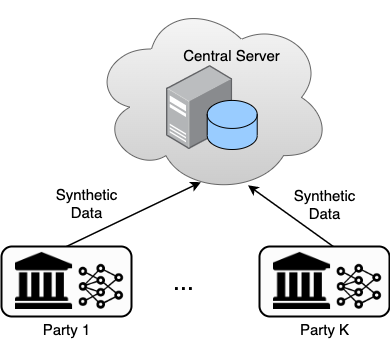
\includegraphics[width=\textwidth]{Plots/local_training.png}
		\caption[]%
		{{\scriptsize Local Training }}
 	\label{fig:local_level}
 		\end{subfigure}
	\hfill
	\begin{subfigure}[b]{0.42\linewidth} 
		\centering
		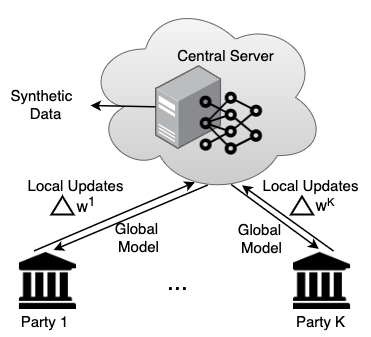
\includegraphics[width=\textwidth]{Plots/federated_training.png}
		\caption[]%
		{{\scriptsize Federated Training }}
 	\label{fig:server_level}
	\end{subfigure}
	\caption{\small Approaches to Private Data Synthesis from Decentralized Non-IID Data: note that in both approaches, the central server may be potentially untrusted.}
	\label{fig:local_levelVSserver_level}
\end{figure}


\section{Proposed Approaches}
In this work, we address privacy-preserving data synthesis via GANs in practical settings, where training data $D$ is distributed across $K$ ($K>1$) parties, i.e., $D = \bigcup_{k=1}^{D}D^{k}$,  and local data distributions may be skewed, i.e., non-IID.  We assume that local datasets do not overlap, i.e., $D^i \cap D^j = \emptyset$ for $i \ne j$.  Specifically, we consider two different approaches as shown in Fig.~\ref{fig:local_levelVSserver_level}: (1) local GAN models are trained privately by each party; (2) global GAN models are trained privately in a federated framework. 

%To this end, we focus on two types of solutions for private data synthesis: i) centralized private GAN solution \cite{DPGANXie2018, PrivGAN2019} applied at each party locally and ii) federated solution \cite{Fedprox2018} for GAN. As shown in Fig. \ref{fig:local_levelVSserver_level} both of these solutions guarantee that local party data never leaves the edge device or the local parties don't have to upload their data on the server. More details about the communication and computation complexity of these solutions can be found in the supplementary material.

\subsection{Training GANs Locally}

The first approach allows each party to train local GAN models using private solutions designed for the centralized setting. As a result, privacy protection is provided to local records, independent of external factors. After training, synthetic records sampled from private local generators can be shared with a central server, which forms a repository of synthetic data. 




%This section shows how we synthesized private data from a decentralized non-IID environment utilizing trained centralized private GAN at each local site. For private data synthesis locally, we use DPGAN \cite{DPGANXie2018} and privGAN \cite{PrivGAN2019} as a centralized private GAN solution for each local party.


Specifically, we consider two existing solutions for this approach, i.e., DPGAN~\cite{DPGANXie2018} and privGAN~\cite{PrivGAN2019}.  DPGAN~\cite{DPGANXie2018} applies the DP-SGD method~\cite{DPSGD2016Abadi} in training GAN models, which provides differential privacy guarantees to real samples. %This solution leverages differential privacy's resistance to post-process~\cite{dwork_book} and proposes to only train the discriminator with the DP-SGD method. 
DPGAN has been applied to synthesize a range of data types in centralized settings~\cite{fan2020survey}. However, due to the perturbation introduced by differential privacy, the synthetic samples often show lower quality compared to those of non-private GAN models. 
%Although the discriminator is trained using DP, the generator has the same privacy as the discriminator due to the post-processing aspect \cite{dwork_book}.
%Due to DPGAN's \cite{DPGANXie2018} poorer generated sample quality as compared to non-private GANs, 
Recently, privGAN~\cite{PrivGAN2019} was proposed to defend against membership inference attacks specifically. Its main idea is to reduce the memorization of training samples by training separate GAN models on disjoint partitions along with a privacy discriminator to infer the generator of a given synthetic sample. The overall objective is a weighted sum of those of GAN models and the privacy discriminator, with a multiplicative factor $\lambda$ for the privacy discriminator. Lower $\lambda$ leads to reduced memorization and often lower quality. While privGAN does not provide any privacy guarantees, it reported good utility and efficacy against membership inference~\cite{PrivGAN2019}.

We propose to train DPGAN or privGAN models at each local party with pre-defined privacy parameters, e.g., $\epsilon$ for DPGAN and $\lambda$ for privGAN, in order to provide equivalent privacy protection across parties.  The evaluation measures for utility and privacy will be introduced in the following section. 

% implemented two strategies to provide good quality data while avoiding memorization of the training set: i) training dataset is randomly partitioned to train multiple generator-discriminator pairs and ii) adapted the idea of built-in adversary $D_p$ \cite{MemAttackNasr2018} by inferring which generator produced fake sample and also acts as a regularizer, preventing generators from remembering training samples. So, privGAN has the following problem to optimize. 

% \[\underbrace{ V(G_i , D_i)}_{\text{utility}} + \underbrace{ \lambda R_p(D_p)}_{\text{privacy}} \] 

% Where the 'utility' term optimizes for generated data quality of samples, while the 'privacy' term is for optimization of membership privacy. 


%Here, we train the privGAN and DPGAN models locally for each party. After training locally, the untrusted or central party will put together a global synthetic dataset by randomly sampling from each party's generator. More details about DPGAN and privGAN can be found in \cite{DPGANXie2018} and \cite{PrivGAN2019}, respectively. 








\subsection{Federated GAN Training}


\begin{algorithm}
\DontPrintSemicolon
\SetAlgoLined
\textbf{Server loop:}

\KwIn{total number of parties $\emph{K} \in \mathbb{N}$, total number of rounds $T \in \mathbb{N}$, sampling probability q $\in$ (0, 1], noise scale $\emph{z} \in \mathbb{R^+}$ , clipping parameter  $S \in \mathbb{R^+} $, generator $\theta^{0}_{ G}$ , discriminator $\theta^{0}_{D}$, privacy accountant $ \mathcal{M}$ }

\text{Initialize} $\sigma = \frac{zS}{qN}$ \;

\For{\text{round} $t=0$ in $T-1$}  
{
	$C^{t}  \leftarrow   \text{ (randomly sample $qN$ distinct parties)}$ \;
 
	\For{$  \text{each party } k  \in C^{t} $} 
 {
		$\Delta^{t+1}_{k} \leftarrow  \text{LocalDiscUpdate}(k, \theta^{t}_{D} , \theta^{t}_{G})$
		\tcp*[l]{compute local update} } 

$\Delta^{t+1} \leftarrow  \frac{1}{qN}  \sum_{k\in C^{t}}^{} \Delta^{t+1}_{k} $\;
 
$\theta^{t+1}_{D} \leftarrow   \theta^{t}_{D} +  \Delta^{t+1} + \mathcal{N} (0,I \sigma^{2})$ \tcp*[l]{update discriminator privately} 
$\mathcal{M}\text{.accum-privacy-spending($z$)}$\;

$\theta^{t+1}_{G} \leftarrow  \text{GeneratorUpdate}(\theta^{t+1}_{D} , \theta^{t}_{G})$\;
}
$\mathcal{M}\text{.accum-privacy-spent()}$ \tcp*[l]{report total privacy}

\noindent\rule{8cm}{0.4pt}
\BlankLine
\textbf{LocalDiscUpdate$(k,\theta^{t}_{D},\theta_G)$:} 

\KwIn{batch-size $B \in$ $\mathbb{N}$, number of disc. steps $n$ $\in \mathbb{N}$, disc. learning rate $\eta_D$ $\in \mathbb{R^+}$, clipping parameter $ S \in \mathbb{R^+}$ , weight for proximal term $\mu \in \mathbb{R^+}$ }

$\theta_{D} \leftarrow   \theta^{t}_{D}$\;

$ \mathcal{B} \leftarrow \text{(sample $n$ size-$B$ batches from real data $D^k$ )}  $ \;

\For{$  \text{each batch }  b_{real}  \in \mathcal{B}$} {
$b_{fake} \leftarrow \text{(sample $B$ synthetic records from generator $\theta_G$)}$\;

$\nabla h  \leftarrow  \nabla h_{\mu} (\theta_D)$  \tcp*[l]{as in~(\ref{eq:proxloss}), parameterized with $\theta^{t}_{D}$, $b_{real}$, $b_{fake}$}
$\theta_D \leftarrow \theta_D - \eta_D  \nabla h  $ \tcp*[l]{local update}
	}
$\Delta = \theta_D - \theta^{t}_{D}$  \;

$ \text{return }\Delta_{k}= \Delta .  \text{min}(1,\frac{S}{||\Delta|| }) $ \tcp{clip locally} 
\BlankLine
\noindent\rule{8cm}{0.4pt}
\BlankLine
\textbf{GeneratorUpdate$(\theta_D, \theta^{t}_{G})$:}

\KwIn{batch-size $B \in \mathbb{N} $, number of gen. steps $n \in \mathbb{N}$,   gen. learning rate $\eta_{G} \in \mathbb{R^{+}}$}
$\theta_{G} \leftarrow \theta^{t}_{G}$ \;

\For{$  \text{each  step from } i=0 \text{ to } n$} {
$b_{fake }  \leftarrow  \text{(sample $B$ synthetic records from generator $\theta_G$)}$\;

$\theta_G \leftarrow  \theta_G - \eta_G \nabla l_G (\theta_G$) \tcp*[l]{update generator, $l_G$ parameterized with $\theta_D$ and $b_{fake}$}
}
	
$ \text{return } \theta_G$
\caption{DP-FedProx-GAN}
\label{alg:dpfedproxgan}
\end{algorithm} 


Federated learning has emerged as a promising solution for jointly training machine learning models while the input data is distributed across multiple parties. One advantage of the federated learning paradigm is that it eliminates the need for sharing input data with external parties, making it easier to comply with local privacy policies and regulations. Our second approach adopts the federated paradigm in which all parties jointly train a pair of generator and discriminator with differential privacy. Synthetic samples can be drawn from the global generator once training is complete. 

Prior work has incorporated differential privacy in the FedAvg algorithm~\cite{DPFedAvg2018}, where each user's participation in federated learning is protected. In this work, we propose to address the non-IID data challenge in federated learning with the FedProx algorithm~\cite{Fedprox2018} and modify the training procedure to learn GAN models with differential privacy. Algorithm~\ref{alg:dpfedproxgan} depicts our proposed solution, namely DP-FedProx GAN.  

The advantage of DP-FedProx GAN is that it achieves user-level privacy by performing local clipping for gradient updates at each party (as in \texttt{LocalDiscUpdate}), followed by global aggregation and perturbation (as in \texttt{Server loop}).  Note that it has been shown that differential privacy can be achieved by training only discriminators privately~\cite{DPGANXie2018} (i.e., clipping and perturbations are not required for training generators), thanks to differential privacy's resistance to post-processing. 

Furthermore, DP-FedProx GAN tackles the significant variability in local data by adding the proximal term to the objective. %To deal with decentralized non-IID data with FL, we propose DP-FedProx GAN; an FL algorithm \cite{Fedprox2018} for GAN training using user-level differential privacy as described in \cite{DPFedAvg2018}. DP-FedProx GAN focuses on user-level differential privacy, which means that the privacy guarantee applies to all of a user's data rather than just a single training sample. Moreover, %DP-FedProx GAN tackles the significant variability in terms of the characteristics and size of local party data by using the proximal term $\mu$. %\textcolor{red}{Could you double-check the following sentences including the equation, for completeness and correctness? Also, later on in the paper, you used $i$ as index for each party, should consider using consistent variable here. } \textcolor{red}{Done }\textcolor{red}{Not done! the equation is missing half parenthesis and the index is still $k$ instead of $i$! }
Specifically, instead of just minimizing the discriminator loss $l_{D}(.)$ as defined in~(\ref{eq:ganobj}), each party $k$ employs its local procedure to minimize the following objective approximately at round $t$:
\begin{equation}\label{eq:proxloss}
	\begin{multlined}
         \min_{\{\theta\}} h_{\mu}(\theta_D) = l_{D}(\theta_D) + \frac{\mu}{2} || \theta_D-\theta^{t}_{D} ||^2
        		% \min_{\{w\}} h_i(w;w^{t}) = F_i(w) + \frac{\mu}{2} || w-w^t ||^2
	\end{multlined}
\end{equation}
The proximal term aims to address both systems and statistical heterogeneity by limiting local party updates closer to the server's global model, hence improving training stability. To assess the efficacy of our proposed solution, we compare it with the existing approach DP-FedAvg GAN~\cite{FedavgGAN2019} in the empirical evaluation. 

%discussed in conclusion section \textcolor{blue}{FedCurv \cite{shoham2019overcoming} is an alternative federated learning algorithm that addresses catastrophic forgetting \cite{goodfellow2013empirical} by adding a penalty term to the loss function, encouraging convergence of local models towards a shared optimum. However, compared to FedAvg and FedProx, it may exhibit drawbacks such as higher computational complexity, and increased communication required to exchange Fisher Information Matrix among participating clients.}







% \begin{algorithm}[tb]
% \caption{Private data synthesis: At server level}
% \label{alg:DP-FedProx GAN}
% \textbf{Input}: K, T, µ, γ, w 0 , N, pk, k = 1, · · · , N\\
% \begin{algorithmic}
% \FOR{t=0,...T-1}
% % \STATE Server selects a subset $S_t$ of K devices at random (each
% % device $k$ is chosen with probability $p_k$)
% % \STATE Server sends $w^t$ to all chosen devices
% % \STATE Each chosen device $k$ \in $S_t$ finds a $w_k{^{t+1}}$ which is a γ -inexact minimizer of: \min_{\{w\}} h_k(w;w^{t} = F_k(w) + \frac{\mu}{2} || w-w^t ||^2 
% % \STATE Each device $k$ \in $S_t$ sends $w_k{^{t+1}}$ back to the server
% % Server aggregates the w’s as $w{t+1}$

% \ENDFOR
% \end{algorithmic}
% \end{algorithm}


\subsection{Non-IID Data Simulation}

Non-IID data distributions may pose significant challenges in decentralized machine learning applications~\cite{HsiehNonIIDData2019}. Recent research has explored partitioning techniques~\cite{kairouz2021advances} to quantify and control the imbalanced features of decentralized datasets, which is beneficial for developing and validating new machine learning algorithms. Inspired by prior research, below we discuss various types of distributions considered in this work. 


%Non-IID is a critical and prevalent data challenge while building learning ML algorithms for decentralized data. In recent years, there has been a rise in interest in leveraging distributed databases to improve machine learning models. However, because of rising privacy concerns and data restrictions such as the GDPR, sharing raw data among organizations and nations may become difficult or risky. For example, due to different data restrictions between nations, multinational organizations are often not permitted to exchange one country's individual data with another. Another data challenge for developing ML models from decentralized databases is that local data distribution can be non-IID and pose significant challenge in decentralized learning \cite{HsiehNonIIDData2019}. For instance, the ozone layer may cause one hospital in the Southern Hemisphere to have more data on skin cancer patients than other hospitals in other locations.

%For private data synthesized from real-world scenarios, i.e., decentralized non-IID data, we partition the real-world dataset into multiple smaller subsets. Furthermore, assessing the imbalance properties, i.e., imbalanced level and imbalanced case, in real federated datasets \cite{HufederatedD2022, CaldasfederatedD2018} is difficult. On the other hand, Partitioning techniques can easily quantify and control the imbalanced features of local party data. Thus, researchers may easily explore learning algorithm behavior by experimenting with various unbalanced settings, which is critical in the building of learning algorithms. From a non-IID distribution perspective, an existing research study \cite{NonIDD2019} provides a comprehensive summary of non-IID data situations. The following subsections discuss the various skew distributions across parties used in our experiments.

\partitle{Non-Skew (NS)} We use the non-skew  distribution as a baseline. In NS, each party has an equal-sized subset sampled uniformly at random from the overall training data.  
%data is uniformly randomly distributed among all parties. 

\partitle{Quantity Skew (QS)} In quantity skew, the size of each party's dataset $|D^k|$ varies, without varying the label distribution. We use the Dirichlet distribution as in~\cite{DistImabalance2019, DistLabelWang2020,DistLabelQinbin2021,Silos2021} to simulate the skewed quantities among parties. 
%Although data distribution across the parties may still be consistent, analyzing the effect of quantity skew in different private data synthesis solutions based on decentralized non-IID data is interesting. To stimulate real world distrubutions i.e non-IID, usually Dirichlet distribution is used \cite{NonIDD2019}. 
%In Bayesian statistics, the Dirichlet distribution is widely used as a conjugate prior for the multinomial distribution \cite{dirichlet20015} and can be thought of as a multivariate version of the Beta distribution. It is often used to simulate real-world data distribution. Many recent research studies \cite{DistLabelQinbin2021,DistLabelWang2020} have adopted this partitioning technique. 
Formally, the probability density function for Dirichlet distribution is defined as follows:
\begin{equation}
 Dir_{K,\alpha}(x)= \frac{1}{\mathrm{B}(\alpha )} \prod_{k=1}^{K} x_{k}^{\alpha -1} \text{ where } \mathrm{B}(\alpha)= \frac{\prod_{k=1}^{K}\Gamma (\alpha_{k}) }{\Gamma (\sum_{i=k}^{K}\alpha_{k})}
\end{equation}
in which $x$ is a $K$-dimensional variable and $\alpha =(\alpha_{1},...,\alpha_{K})$ representation concentration parameters. For simplicity, we assume the same concentration parameter for every $k$. To simulate different data quantifies across $K$ parties, we draw $q \sim$ $Dir_{K,\alpha}$ and assign $q_{k}$ proportion of training data to $D^k$. We can control the amount of quantity imbalance by varying the $\alpha$ value. A smaller $\alpha$ leads to a higher imbalance and vice versa, as shown in Fig.~\ref{fig:dirichlet_beta_vary}. 



\begin{figure}
 \centering
 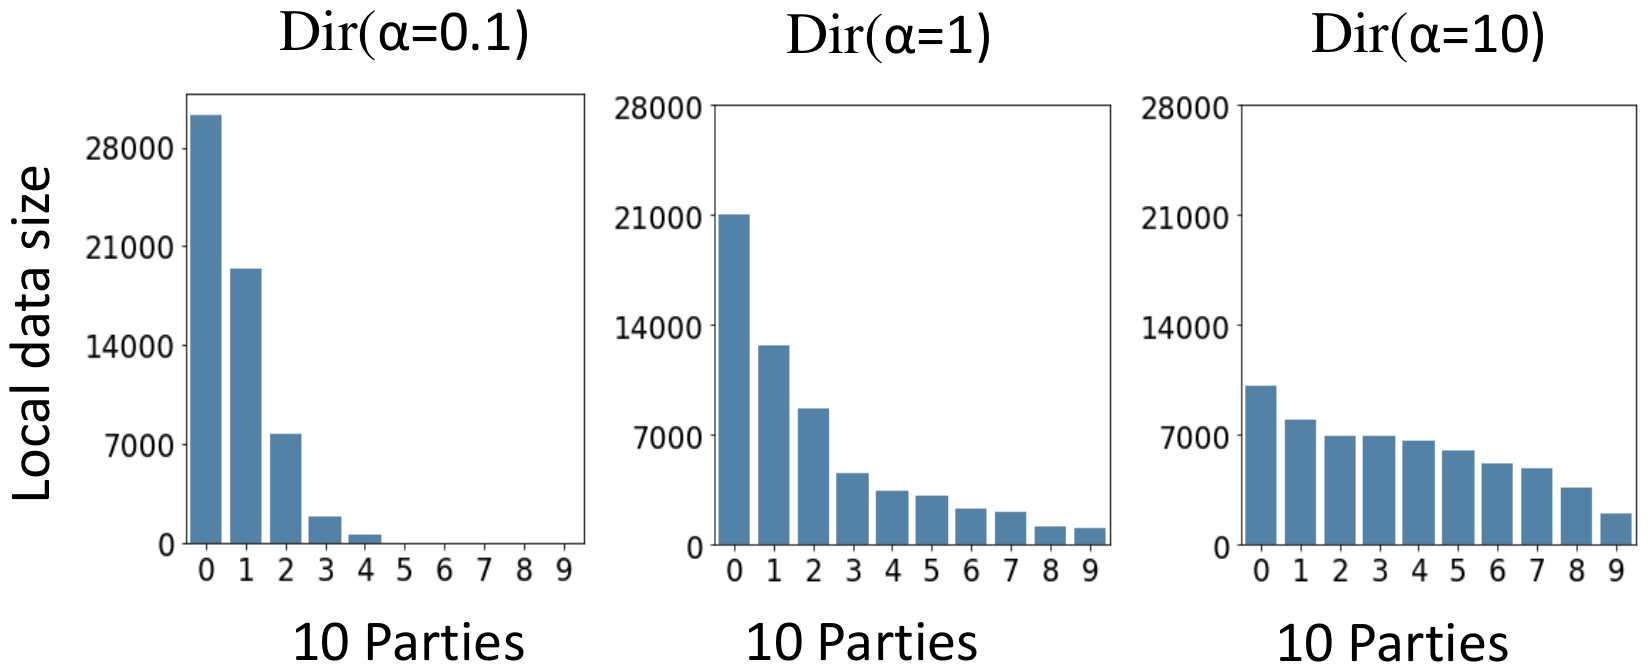
\includegraphics[width=0.95\linewidth]{Plots/dirichlet_beta_vary.png}
 \caption{Examples of Quantity Skew: simulated 10 parties with the MNIST dataset by varying $\alpha$ in Dirichlet distribution.}

 \label{fig:dirichlet_beta_vary}
\end{figure}

%Here, we utilize the same Dirichlet distribution to assign varying numbers of data samples to each local party. For this, we simulate $q \sim$ \emph{Dir_{P}($\alpha$)} and assigned $q_{j} $ proportion of whole data to party $P_{j}$. Here, f(x) shows the probability density function of parties for stimulated, i.e, $Dir_{P}$. 

%\subsubsection{Label Distribution Skew} 

%In Label Distribution Skew, each label distribution P($y_i$) is different among parties. In the real world, hospitals may deal with a particular disease and be required to generate synthetic data for a specific type of medical record. For example, one hospital may specialize in treating particular diseases and have more patient data on them. To deal such scenarios, we experiment with two labels imbalance settings: quantity-based label imbalance and distribution-based label imbalance.\linebreak 
\partitle{Quantity-based Label Imbalance (QLI)} Besides quantity, the label distribution may vary from one party to another. Some studies~\cite{FLMcMahan2016, DistImabalance2019} noted that local data may contain different subsets of labels. {For example, one party may have samples from classes 1 and 2, while another may have samples from classes 2 and 3. } To simulate quantity-based label imbalance, we assign 3 classes to each party and randomly assign samples of those classes to the party as in \cite{Silos2021}. Note that the quantities of local data are balanced in this setting. 

%In quantity-based label imbalance (QLI), each party owns a set number of labeled data samples as studied in \cite{FLMcMahan2016, DistImabalance2019}. In this way, each party has a different number of samples of \emph{K} different labels. After assigning \emph{K} labels to every party, we uniformly and randomly assigned samples of each label to the respective assigned parties without any overlap across parties. In our experiments, we use \emph{\#Labels=3} for assigning \emph{K} labels to each party. 
%\linebreak 
\partitle{Distribution-based Label Imbalance (DLI)} In distribution-based label imbalance, samples of each label is distributed non-IID across the parties. 
%each party has the proportion of samples of each label according to Dirichlet distribution . 
For each label $j$, we draw $p^j \sim Dir_{K,\alpha}$ and assign $p^j_k$ proportion of samples of label $j$ to party $k$ as described in ~\cite{Silos2021}. %Dir($\alpha$) represents the Dirichlet distribution, and $\alpha$ specifies the concentration parameter of the distribution ($\alpha$ must be positive i.e $\alpha >0 $). The parameter $\alpha$ can be used to modify the amount of skew for label proportion $p_{k,j}$ for parties.
Note that in DLI, both the quantity and the label distribution of the local dataset may differ between one party and another.  

%To represent these partitioning strategies, we use \emph{NS} for Non-Skew, \emph{QS} for Quanity Skew, \emph{QLI} for Quantity-based label imbalance, and \emph{DLI} for Distribution-based label imbalance for simplicity. 

\section{Evaluation Measures of Data Synthesis}
In this section, we describe a number of quality and privacy measures adopted in evaluating data synthesis solutions. As a proof of concept, this study focuses on image data, while the proposed private data synthesis solutions can be generalized to other domains. 

\partitle{Utility Metrics}
%In utility evaluation, we examine the impact of hyperparameter selection on the quality of synthetic data. For this, the central party needs a global synthetic dataset from local parties to access the qualitative quality of generated data. In the case of centralized private GANs (privGAN and DPGAN) applied locally, the central party gathers the generated data from local parties by randomly sampling each generator(s) $G_i$ of the local party. On the other hand, in federated solution (DP-FedProx GAN), synthetic data is generated by the central server. 
% 
To simulate human evaluation of synthetic samples, strategies for assessing the realism and diversity of generated data have been developed for GANs. Among them, Inception Score (IS) \cite{InceptionScore2016}, and Fréchet Inception Distance (FID) \cite{FidScore2017} have been extensively evaluated in the literature. The IS captures the KL divergence between the conditional label distribution (estimated with the Inception model) and the marginal distribution for synthetic samples. The FID computes the Fréchet distance between the distributions of real data and generated data. %It is known that IS does not capture intra-class variability and is unaffected by prior distribution of labels, while FID is sensitive to small changes in the real distribution (e.g., slight blurring or small artifacts in synthesized images) and can identify intra-class mode collapse\cite{ProsConsEval2021}.


%For IS, we use the inception model~\cite{InceptionV3_2015} to obtain the conditional label distribution $p(y|x)$ of each generated sample. If x is similar to a real sample, the entropy of $p(y|x)$ should be low. Furthermore, we expect that the generator \G will generate a diverse set of samples, therefore the marginal distribution \(\int_{}^{} p(y|x = G(z)) \,dz\) should have a large entropy. Combining these two requirements, IS measures the KL divergence of the these two distributions by computing \( exp \Bigl( \mathrm{E}_{x \sim G(z)} (KL(p(y|x)||p(y))) \Bigl) \). We capture both the quality and diversity of the synthetic data in this manner. On the other hand, FID computes the difference between the distribution of real data $P_{real}$ and generated data $P_G$. Like IS, generated and real images are fed into the inception model \cite{InceptionV3_2015}, and it assumes that their outputs follow Gaussian distribution. The difference between these two Gaussians is measured by the Fréchet distance \cite{FrechetD1982} to compute FID. IS does not capture intra-class variability and is unaffected by prior distribution of labels, while FID is sensitive to small changes in the real distribution (e.g., slight blurring or small artifacts in synthesized images) and can identify intra-class mode collapse\cite{ProsConsEval2021}.

Although the IS and FID scores take into account the unambiguity and relative abundance of distinct classes in generated data, we look at those measures explicitly via entropy and diversity measures as in~\cite{PrivGAN2019}. Entropy is calculated for the conditional label distribution of synthetic samples, which is also estimated using the inception model. The diversity of synthetic samples is computed using the most likely label for each sample in the conditional distribution. 

%them separately by calculating entropy and diversity, respectively, as explained in \cite{PrivGAN2019}. For entropy, the same inception classifier is used to calculate predicted class probabilities to observe the uncertainty in the class of the generated images. After computing entropy for each generated image, we averaged the entropy across all data. A lower average entropy indicates less uncertainty in the predicted image class. Similarly, we identified the most likely class using the same InceptionV3 model for class diversity. For utility evaluation metrics (i.e., IS, FID, entropy, and diversity), the InceptionV3 network classifier \cite{InceptionV3_2015} is tuned for each dataset to achieve reasonable performance. 



\partitle{Membership Inference Risks}
As the proposed solutions adopt various privacy notions, i.e., non-differential privacy, record-level DP, and user-level DP, it is important to evaluate their privacy protection via common empirical measures. An important class of privacy attacks in machine learning is membership inference~\cite{ShokriMemML2016, ChenGANLeaks_2020}. With access to the learned GAN models, the following membership inference attacks may be launched. Although model sharing is not necessary in data synthesis, evaluating those attacks provides insights into the privacy properties of learned models and helps assess the privacy loss in worst cases, e.g., by model stealing. 

We adopt two attacks on GAN discriminators to the decentralized setting, i.e., the white-box (WB) attack~\cite{WBAttack2018} and the total variation distance (TVD) attack~\cite{PrivGAN2019}. In these attacks, an adversary aims to infer whether a sample is used in training the GAN models and does not know the source of the sample, i.e., the party holding the sample.  When GAN models are trained locally, we adapt the original WB and TVD attacks such that the adversary takes the maximum discriminator score over all parties, with the intuition that the discriminator trained with a specific sample will have the highest discriminator score. 

%This section will describe different membership inference attacks targeting generators and discriminators against private GANs trained with decentralized non-IID data.

% \subsubsection{Attacks on discriminator}
% The attack on the discriminator assumes that the adversary has locally trained models (where centralized private GANs are trained locally) or a global model (in DP federated GANs). Along with the trained model(s), the adversary has access to a large amount of data, including training samples. This paper focuses on two types of discriminator(s) attacks: i) White-box attack and Total Variation Distance attack. 

% % \subsubsubsection{ \textbf{White–box attack on discriminator}}
% \cite{WBAttack2018} proposes a white-box (WB) attack on GANs based on the assumption of knowing what proportion of the dataset was utilized for training. In DP-FedProx GAN, the server has a global discriminator, so we use it solely for evaluating white-box attacks in multiple-party settings, as described by \cite{WBAttack2018}. Since every party possesses its own local model and its knowledge is not shared with any third party in centralized private GANs trained locally, the \cite{WBAttack2018} cannot be applied directly to it. So, for a successful white–box attack in a multiple-parties setting, the adversary passes every sample of its possessed data from the local party discriminator and obtains a probability score. Since every party \K has a discriminator ( $N=2$ discriminators in privGAN for each party), we take a max over the scores from all discriminators of parties. The reasoning is that the discriminator trained with a specific sample will have the highest discriminator score. The scores are then sorted in descending order, with the top $f$ percent of the scores being outputted as the likely training set. In the end, we examine how much of the predicted training set was used in the model's training.
% % \subsubsubsection{ \textbf{Total Variation Distance attack on discriminator}}


% As explained in \cite{PrivGAN2019}, we use Total Variation Distance (TVD) to robustly evaluate the effectiveness of an attacker who solely utilizes discriminator scores. For TVD, we calculate the difference between two distributions of discriminator scores for $X_{train}$ and $X_{ho}$(holdout set). Since there are not enough examples available for training in practical settings, we bin the discriminator scores into evenly spaced bins and compute the TVD on the resultant distributions. Due to multiple discriminators spanning multiple parties, this attack, like the white-box attack on the discriminator, does not operate directly on centralized private GANs trained at each party locally. As a result, we modify the approach by calculating the maximum TVD of the distribution of discriminator scores for $X_{train}$ and $X_{ho}$ overall discriminators.


%\subsubsection{Monte–Carlo attack on generator}

The generator in GANs is also prone to set membership inference in Monte–Carlo (MC) attacks~\cite{MCAttackHilprecht2019}. In the MC attack, the adversary's objective is to determine whether a given set of samples are part of the GAN models' training set or synthetically generated. It computes the similarity between samples in each set using PCA transformation and preserves 40 principal components.  The MC attack can be readily evaluated using synthetic samples drawn from locally trained GAN models as well as federated GAN models. 

%In Monte–Carlo (MC) attacks, we have two sets; one with desired membership(part of the model's training set) and the other without desired membership(synthetic dataset). Here, the adversary's goal is to determine whether a given set has desired membership. The Monte–Carlo attack works by the availability of $n$ synthetic samples generated by generator(s) or the generator(s) generated $n$ synthetic samples. In the case of centralized private GANs, i.e., privGAN and DPGAN, trained locally at each party, every party generates synthetic samples. On the other hand, DP-FedProx GAN central server generates synthetic samples. After generating synthetic data, we compute $\frac{1}{n} \sum_{i=1}^{n} 1_{x_i \in U_{S_i \in }, (x_i) } $ where $U_{\in}(x) = {\acute{x}| d(x,\acute{x}) \le \epsilon } $ for each sample in the two sets whose memberships are being evaluated. As explained in \cite{MCAttackHilprecht2019}, we use PCA transformation (with the first 40 components) to find out the euclidean distance between two images $x$ and $\acute{x}$. More details can be found in \cite{MCAttackHilprecht2019}.





\section{Experiments}

%In this section, we will show detailed experiments to evaluate how the privacy level, concentration parameter, and a number of parties influence the utility and privacy risk in private data synthesis from decentralized non-IID data. In our experiments, centralized privGAN and DPGAN imply that they are applied at each party locally for private data synthesis from decentralized non-IID data. For all these solutions, utility evaluation is done at an untrusted/central party after local parties send their synthetic data. Moreover, local parties send private synthetic samples equal to the amount of their local data to an untrusted/central server. As a result, local data holders with more synthetic data contribute more to utility evaluation. On the other hand, DP-FedProx is a federated solution where the central server generates synthetic data.

In this section, we present the evaluation methodology and empirical results on the proposed data synthesis solutions.  

% Due to limited space, we report additional details and experiments in the Appendix which is provided via an anonymous link online\footnote{For blind review, we present the anonymous link to \url{https://drive.google.com/file/d/1wDv6QOz9lJk9sUe3t_yfbN8KLdhFxtof/view}}.  

\partitle{Datasets} Our experiments adopt the following datasets: MNIST, Fashion-MNIST(f-MNIST), CIFAR-10, and CelebA. Note that to create a balanced dataset, we sub-sampled the original CelebA~\cite{CelebAData2014} to obtain 30 images per identity for 1000 celebrities.  We also center-cropped each image to obtain face regions of 48 $\times$ 48 pixels. %They have a balanced number of images from 1000 different image classes.
% The GAN model details for each dataset are provided in the {online appendix}. 

\partitle{Approaches} We evaluate several approaches, i.e., local training of privGAN and DPGAN models and our proposed DP-FedProx GAN. In addition, we include DP-FedAvg GAN~\cite{FedavgGAN2019}, which is the current solution for training GAN models in decentralized settings.  It is important to note that we also consider an alternative approach, namely DP-FedSGD GAN, which learns federated GAN models using the DP-FedSGD algorithm~\cite{DPFedAvg2018}. However, we omit DP-FedSGD GAN from our evaluation, as it requires a higher number of training iterations and performs poorly compared to the other approaches.


% We exclude its results from the main paper and interested readers can find them in the online appendix.

%\textcolor{red}{We also examined the DP-FedSGD-GAN approach to evaluate our proposed DP-FedProx GAN, in which we apply the DP FedSGD approach to learning GAN models. Here, we selected large-batch SGD data from each party, which requires a higher number of iterations to achieve equivalent accuracy, and that comes with a privacy cost \cite{DPFedAvg2018}. Therefore, DP-FedSGD GAN was not considered in our evaluation.  }


\partitle{Default Parameter Values} $\lambda$ and $\epsilon$ parameters specify the degree of privacy protection in privGAN, DPGAN, and DP-FedProx GAN. %For privGAN, our evaluation focuses on range of $\lambda \in [0.1,0.5,1,5,10]$, for DPGAN, we focus on the range of $\epsilon \in [2.1,4.01,8.03,16.05]$ and for DP-FedProx GAN, we use $\epsilon \in [24.01,30.1,42.02,64.11]$ . 
The default values used are $\lambda$=1 in privGAN, $\epsilon$=4.01 in DPGAN, and $\epsilon$=64.11 in DP-FedProx GAN and DP-FedAvg GAN. The default sampling probability $q$ is set to 0.1 in DP-FedProx GAN and DP-FedAvg GAN. For DP-FedProx GAN, $\mu$ in~(\ref{eq:proxloss}) specifies the weight of the proximal term and is set to 0.5.  %Usually, larger $\lambda$ in privGAN and smaller $\epsilon$ in DPGAN and DP-FedProx GAN have little usefulness, but they provide higher privacy protection. 
The concentration parameter $\alpha$ indicates the level of imbalance, and the default value is set $\alpha = 0.5$. %Our evaluation focuses on the range of $\alpha \in [0.1,0.5,1,5,10]$ with a default value of $\alpha$ = 0.5. If $\alpha$ is set to a lower value, the partition becomes more imbalanced. 
The number of parties $K$ is set as $K=10$, unless specified otherwise.  Table ~\ref{Tab:clipping_para} presents clipping parameters $S$ for differentially private solutions in each dataset.

\begin{table}[]
\centering
\begin{tabular}{|c|c|c|c|c|}
\hline
               & MNIST & f-MNIST & CIFAR-10 & CelebA \\ \hline
DPGAN          & 1e-2  & 1e-2    & 5e-2     & 5e-2   \\ \hline
DP-FedProx GAN & 1e-2  & 1e-2    & 5e-2     & 5e-2   \\ \hline
DP-FedAvg GAN  & 1e-2  & 5e-2    & 5e-2     & 5e-2   \\ \hline
% DP-FedSGD GAN  & 5e-2  & 5e-2    & 5e-2     & 5e-2   \\ \hline
\end{tabular}
\caption{Clipping Parameters for Differentially Private Solutions}
\label{Tab:clipping_para}
\end{table}







% FedAvg \cite{FLMcMahan2016} has been demonstrated statistically to diverge empirically in scenarios where the parties have highly skewed non-IID data \cite{zhao2018fedNon_IID}.

% \begin{table}[h]
% \centering
% \resizebox{0.95\columnwidth}{!}{
% \begin{tabular}{|c|c|c|c|c|}
% \hline
%   & MNIST & f-MNIST & CIFAR-10 & CelebA \\ \hline
% Real Data - IS & 9.9 & 9.6 & 9.1 & 141.4 \\ \hline
% IS & 9.2 & 9.0 & 7.8 & 88.8 \\ \hline
% FID & 12.2 & 14.2 & 30.1 & 45.1 \\ \hline

% \end{tabular}}
% \caption{The IS and FID score on real images \& synthetic images generated with centralized non-private GAN (K=1)}
% \label{Tab:IS_FID_Centralized}
% \end{table}
\begin{table}[]
\centering
\resizebox{0.48\textwidth}{!}{


\begin{tabular}{|c|c|c|c|c|c|}


\hline
                                                                                 &     & MNIST & f-MNIST & CIFAR-10 & CelebA \\ \hline

\multicolumn{1}{|c|}{Real Data}                                               & IS                       & 9.9                    & 9.6                    & 9.1                    & 141.4                  \\ \hline

\multirow{2}{*}{\begin{tabular}[c]{@{}c@{}}Centralized GAN\\ ($K=1$)\end{tabular}} & IS  & 9.2   & 9.0     & 7.8      & 88.8   \\ \cline{2-6} 
                                                                                 & FID & 12.2  & 14.2    & 30.1     & 45.1   \\ \hline
\multirow{2}{*}{\begin{tabular}[c]{@{}c@{}}Local GANs\\ ($K=10$)\end{tabular}}     & IS  & 5.5   & 5.20    & 4.12     & 28.30  \\ \cline{2-6} 
                                                                                 & FID & 40.80 & 38.50   & 80.23    & 110.54 \\ \hline
\multirow{2}{*}{\begin{tabular}[c]{@{}c@{}}Federated GAN\\ ($K=10$)\end{tabular}}  & IS  & 8.4   & 8.61    & 5.50     & 39.41  \\ \cline{2-6} 
                                                                                 & FID & 16.21 & 25.50   & 56.41    & 78.45  \\ \hline
\end{tabular}

}
\caption{IS and FID Scores: Real Data, Centralized Non-Private GAN ($K=1$), Non-Private Local and Federated GANs with NS distribution ($K=10$).}
\label{Tab:IS_FID_Centr_NonIID}
\end{table}




%\subsection{Utility}

 
% In this section, we vary the privacy parameters for the studied private GANs and investigate their quantitative effects on utility metrics, i.e., by varying $\lambda$ and $\epsilon$ values. Furthermore, we investigate those impacts under various concentration parameters for different skew distributions by varying $\alpha$ in QS and DLI. Moreover, we also study how increasing parties affect quality metrics with different distributions.
 
\subsection{Varying privacy parameters}

\begin{figure}[ht]
 \centering
 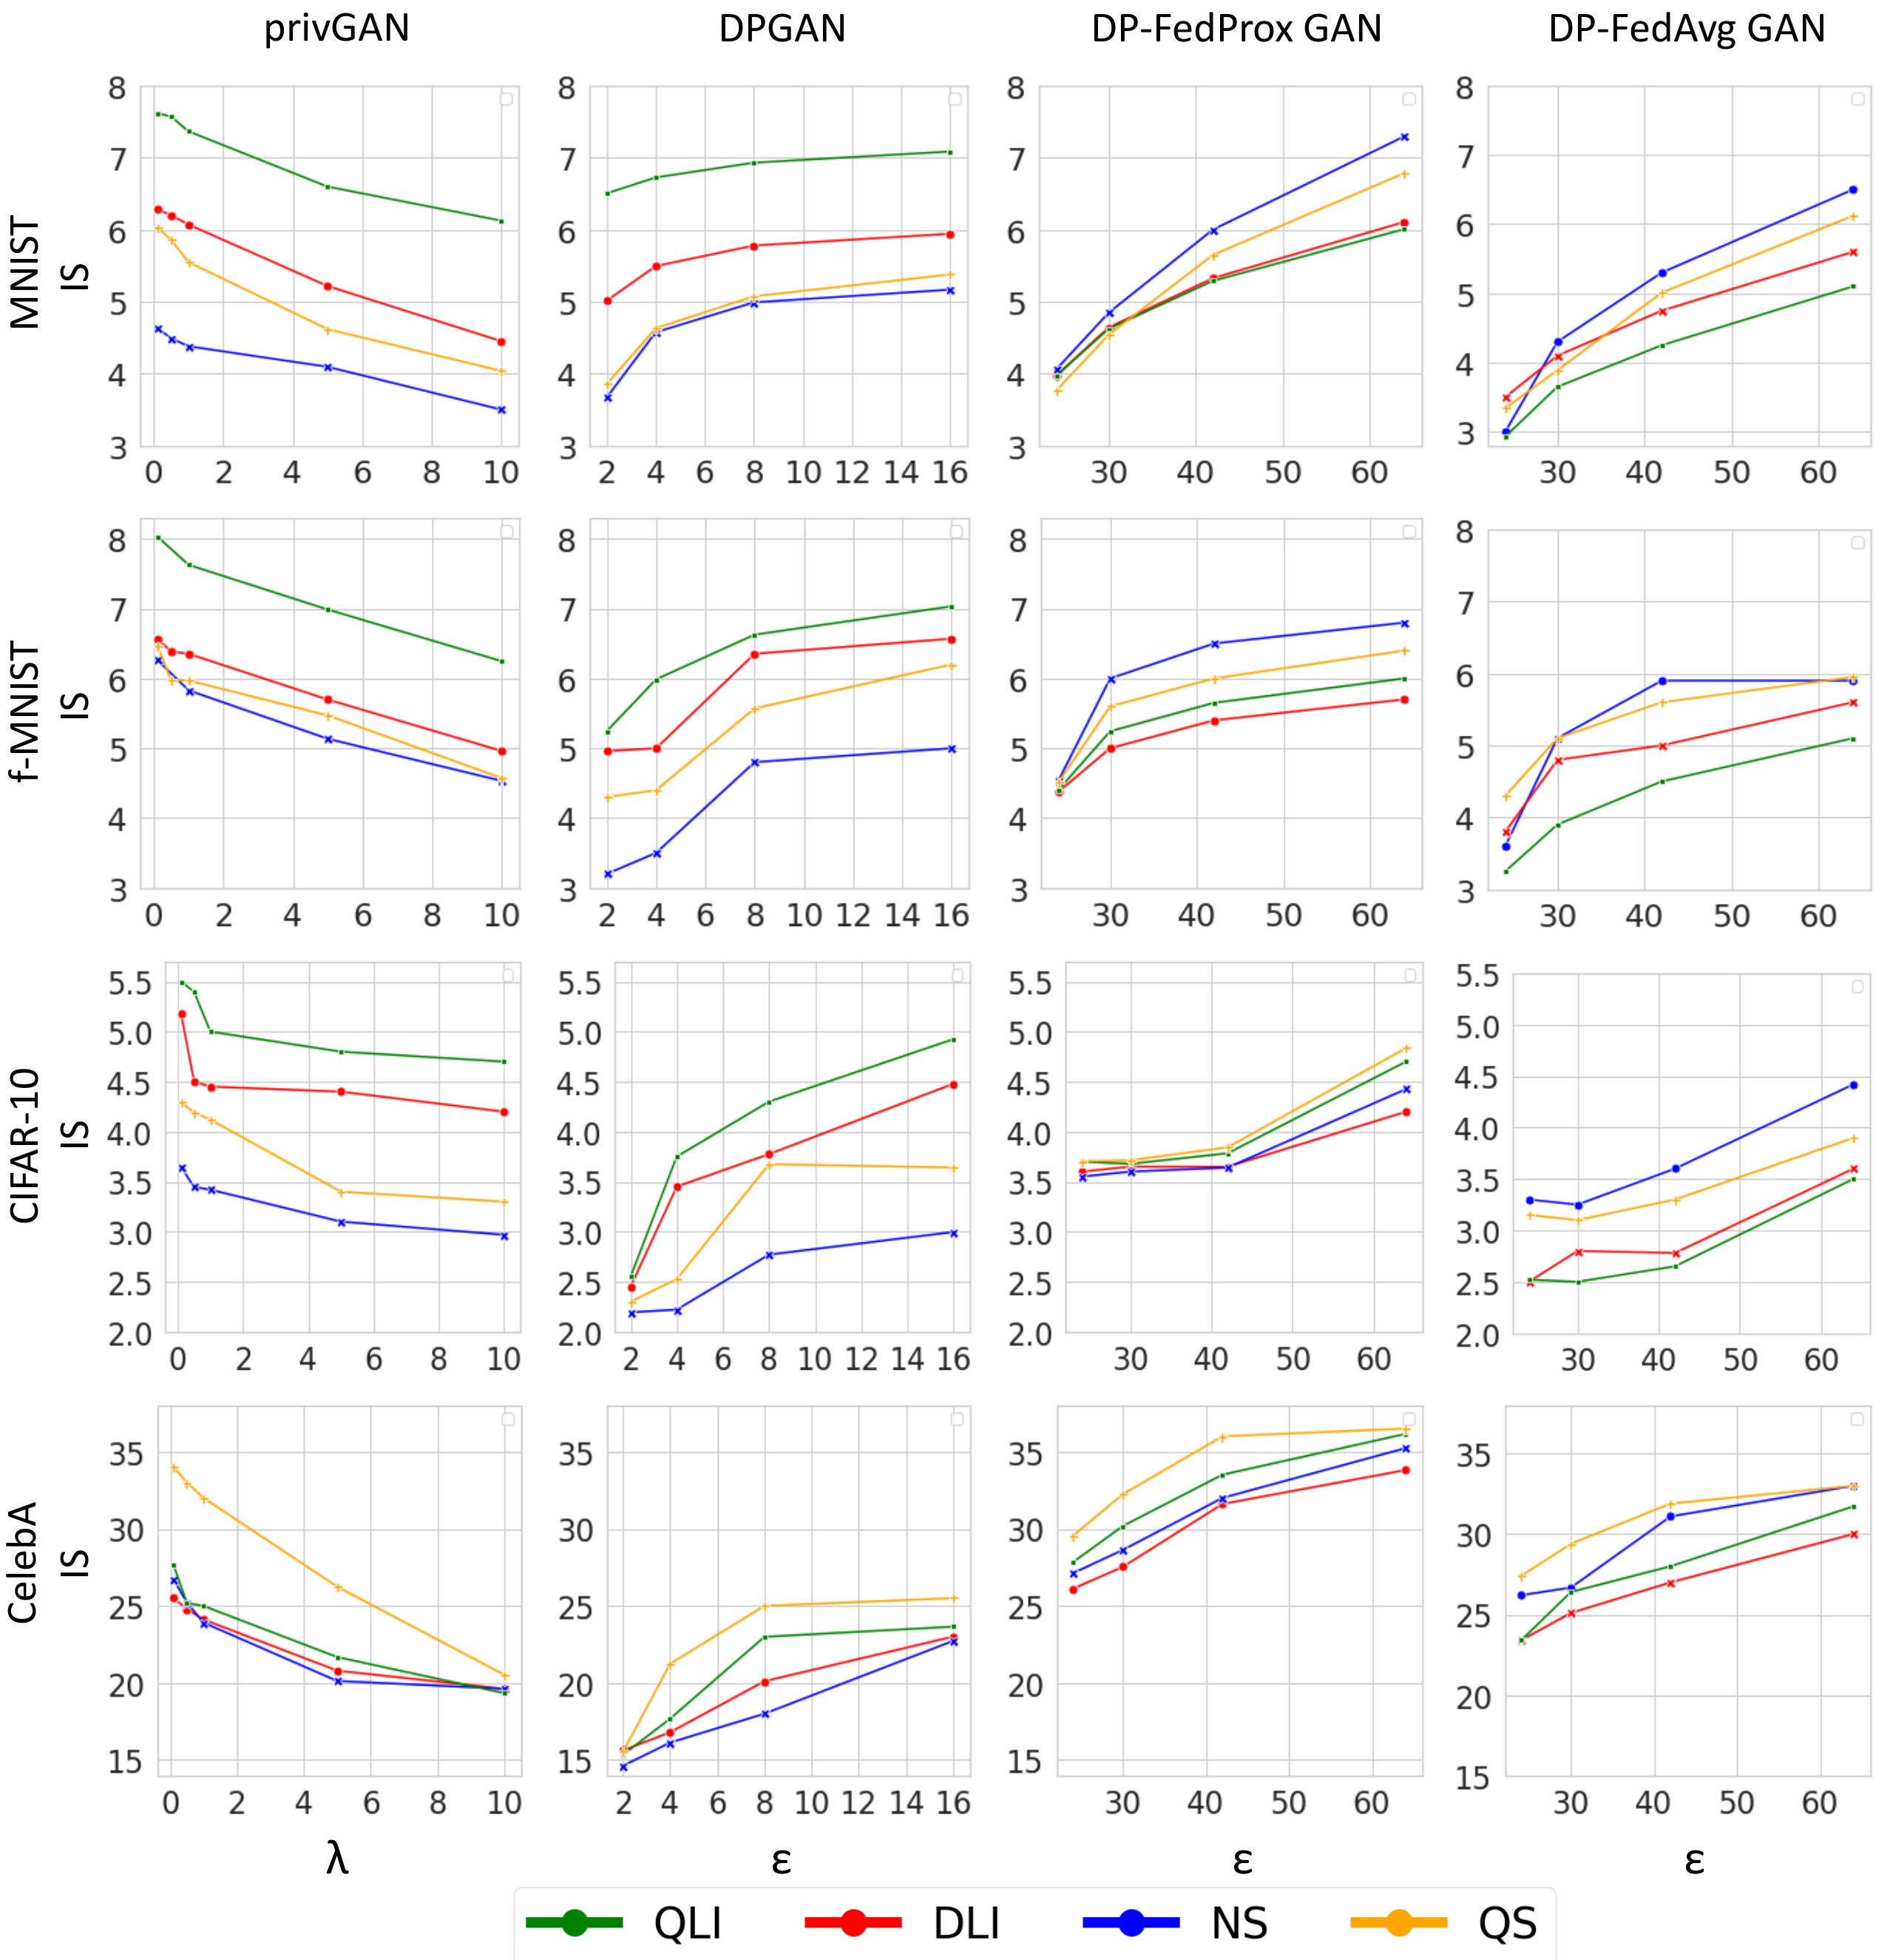
\includegraphics[width=0.48\textwidth]{Plots/varyNoise.png}
 \caption{Varying Privacy Parameters}
 \label{fig:varyNoise}
\end{figure}


\begin{figure}[t]
 \centering
 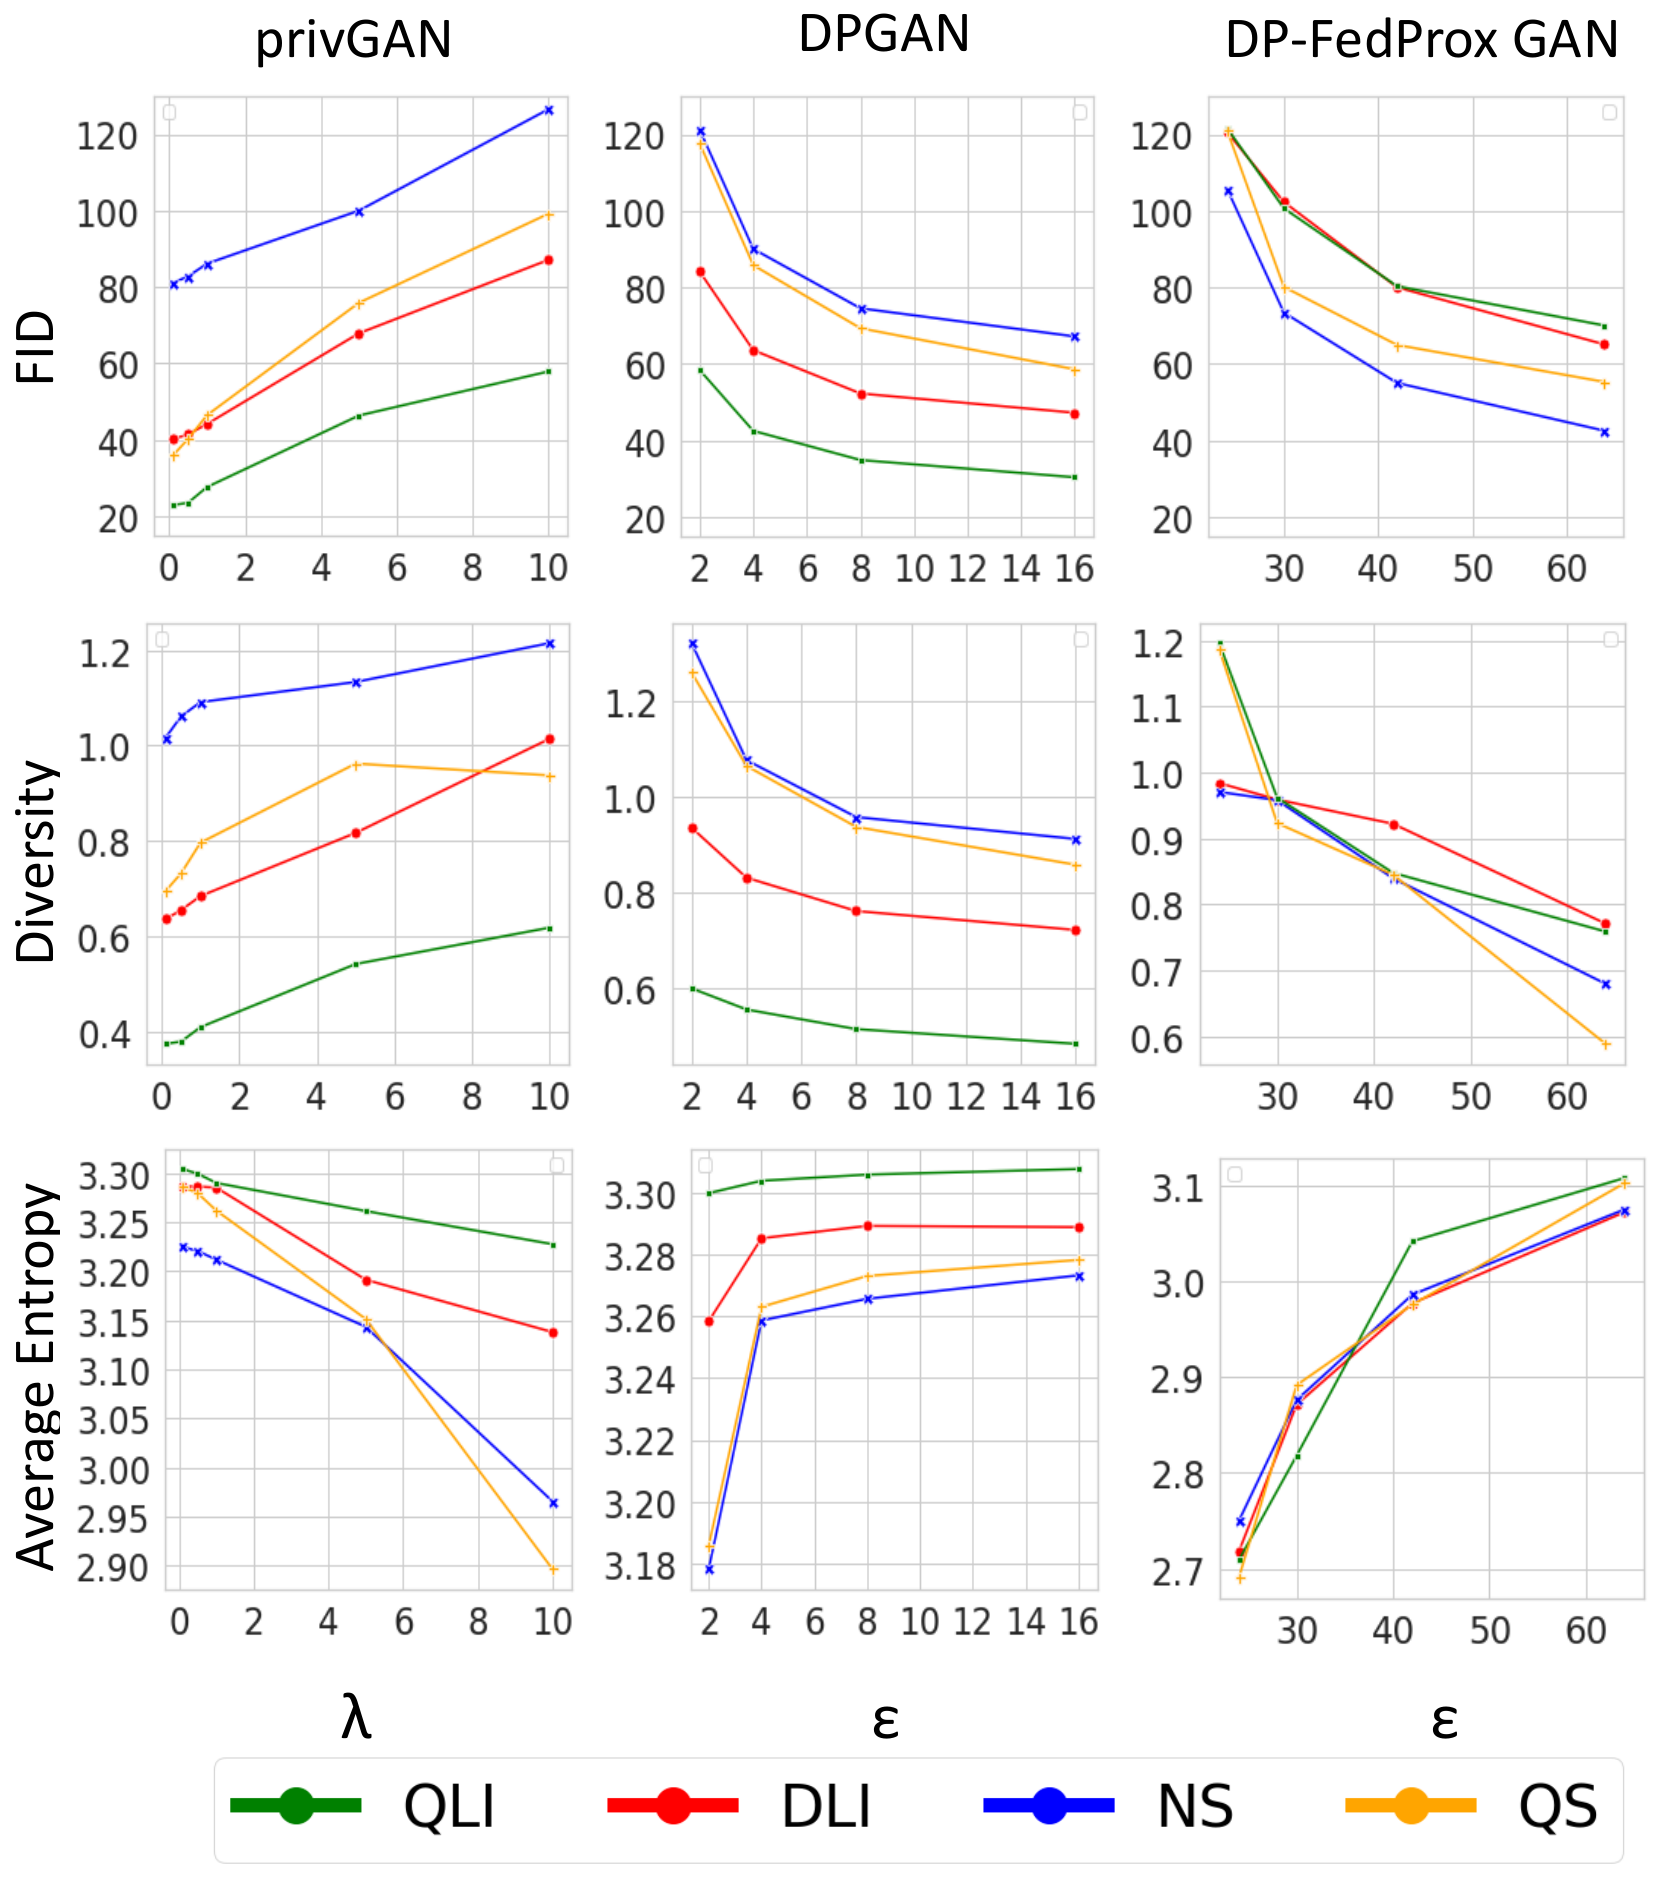
\includegraphics[width=0.90\linewidth]{Plots/entropy_diversity.png}
	\caption{Class Diversity and Average Entropy with MNIST }
 \label{fig:varyNoiseDivEnt}
\end{figure}



 This experiment shows how the privacy parameters of private GANs affect the utility metrics.   {As a reference, we show IS and FID scores for non-private centralized GAN as well as non-private local and federated GAN models in Table~\ref{Tab:IS_FID_Centr_NonIID}}. In comparison to real data and synthetic data generated by centralized GAN, all decentralized GAN solutions lead to high utility loss, i.e., much lower IS scores.  It can be seen that GAN models trained locally suffer from limited data at each party. %\textcolor{blue}{The generation of high-quality images in decentralized settings poses a considerable challenge due to the relatively small size of the CelebA dataset, coupled with its high-resolution image properties.} 
 As CelebA is smaller in size and higher in resolution, it is more challenging to generate high-quality images in decentralized settings. 


Fig. \ref{fig:varyNoise} shows the results of IS measures for all private solutions and all datasets. When we increase $\lambda$ in  privGAN and decrease $\epsilon$ in DPGAN, DP-FedProx GAN and DP-FedAvg GAN, the utility improves monotonically. 
 We observe that training GANs locally (i.e., privGAN and DPGAN) does not learn the underlying distribution of local data well in non-skew (NS) settings. The reason is that none of the local parties holds sufficient data. For example, NS distribution has the lowest utility across all $\lambda$ in privGAN and $\epsilon$ in DPGAN. However, DP-FedProx GAN shows a higher utility with NS, in comparison to non-IID distributions.  As a random subset of local parties participates in each round of training the DP-FedProx GAN, NS distributions can be learned uniformly across parties.  We note that DP-FedProx GAN effectively manages statistical heterogeneity by constraining local updates to be closer to the global model,  as all non-IID distributions yield similar performance to that of NS. {As expected, DP-FedAvg GAN struggles to learn from non-IID data distributions and consistently yields lower utility than DP-FedProx GAN across all datasets. Therefore, we omit DP-FedAvg GAN from the rest of the experiments.}
 
 %We also observe that from $\lambda$= 1 to 5, there is a substantial decline in utility measures in privGAN. 
  %The reason is that the DP-FedProx GAN data availability requirement at each round differs from privGAN and DPGAN. For instance, if selected parties have very few samples in a specific round, other parties with data may fill the gap by updating the global model in the next round. Similar trends of utility metrics are observed across all distributions in DP-FedProx GAN learning. 
In QLI settings, locally trained GAN solutions often lead to good utility because each party focuses on learning only a few classes without encountering mode collapse and instability in GAN training. For instance, QLI has the highest IS for privGAN and DPGAN across all $\lambda$ and $\epsilon$ values, respectively, in MNIST, f-MNIST, and CIFAR-10.  In QS settings, we observe that parties with more data are comparatively more influential (i.e., better utility) for privGAN and DPGAN solutions. QS also leads to better utility in DP-FedProx GAN for the dataset, in comparison to other distributions.   %The federated solution is preferable for these challenges due to the federated learning nature, e.g., DP-FedProx GAN has a considerable overall difference in utility from private GANs applied locally. 


 In Fig. \ref{fig:varyNoiseDivEnt}, we report the effects of privacy parameters on FID score, class diversity, and average entropy with the MNIST dataset.  As $\lambda$ increases in privGAN  and $\epsilon$ decreases in DPGAN and DP-FedAvg GAN, both FID  and entropy increase, and diversity decreases accordingly.  QLI shows the highest class diversity and the lowest FID and average entropy for PrivGAN and DPGAN solutions. Again, all distributions yield similar performances in DP-FedProx GAN, indicating its efficacy in addressing non-IID distributions.
 
 % Additional results, including those with other datasets and DP-FedSGD GAN, can be found in online appendix.




 
 % This experiment shows how privacy parameters affect the utility metrics on private data synthesis. To this end, we vary the privacy parameters for different private data synthesis solutions. Fig. \ref{fig:varyNoise} shows the results of how privacy affects utility studied datasets. When we vary the privacy controlling parameters such as $\lambda$ increases (in privGAN) or $\epsilon$ decreases in (DPGAN and DP-FedProx GAN), IS decreases and FID increases monotonically. Generally, the reduction in IS is accompanied by an increase in FID score. This implies that the class ambiguity of the generated data increases, and the diversity of the data decreases.

% The small amount of data at the local party may work for updating local updates, and another reason is local parties collaboratively make updates to the local model. 
 

 % We observe that if all parties have equal amount of data i.e NS, centralized private GANs (i.e privGAN and DPGAN) applied locally are not learning the underlying distribution of local data. For example, NS distribution has the lowest utility across all $\lambda$s in privGAN and $\epsilon$s in DPGAN because all parties need more data in learning distribution. In MNIST, at $\lambda=$0.1, privGAN has a substantial IS difference of 3.23 between NS and QLI. However, in DP-FedProx GAN, randomly selected parties should have enough data at each round to update the local model so that these local changes can contribute to the global model. As seen in Fig. \ref{fig:varyNoise}, for larger $\epsilon$ values in DP-FedProx GAN, i.e., $\epsilon>=42.02$, the NS distribution has higher IS and lower FID than other skewed distributions in MNIST, and f-MNIST.
 




% A local private GAN solution may easily learn distribution with enough data and fewer classes, i.e., QLI distribution. The reason is each party focuses on a few classes to learn in this situation, making the GAN optimization problem easy. QLI has the largest IS and lowest FID score for privGAN and DPGAN across all $\lambda$ and $\epsilon$ values in MNIST, f-MNIST, and CIFAR-10. For privGAN, there is a considerable difference between QLI and other distributions in MNIST and f-MNIST. In MNIST, f-MNIST, and CIFAR-10, On the other hand, DLI and QS perform on average in terms of utility in private GANs such as privGAN and DPGAN. DLI has a low IS and a high FID score in DP-FedProx GAN. 


 
 % As CelebA has more classes (1000), and each class has a limited number of samples (30), making it challenging for local parties to generate high-quality images with little data. We see in Table \ref{Tab:IS_FID_Centralized} and Fig. \ref{fig:varyNoise} that private data synthesis from decentralized CelebA has significant difference in utility i.e IS, than non-private GAN in a centralized GAN learning context. This is the reason QS distribution is more helpful for GANs learning for complex datasets. Although CelebA doesn't have good utility overall, QS still outperforms other distributions at all $\epsilon$ values in DP-FedProx GAN. For example, in Fig. \ref{fig:varyNoise}, QLI, DLI, and NS have much lower IS and greater FID at $\lambda \le 5$ in privGAN. DP-FedProx GAN has a considerable overall difference in utility from private GANs applied locally for each party. 




 % We can see that from $\lambda$ 0.1 to 1, there is no substantial decline in utility measures in privGAN. Conversely, a significant utility decline from $\lambda$ 1 to 5 represents less diverse and poorly generated data. Fig. \ref{fig:varyNoise} illustrates that at lower privacy budget$\epsilon=$4.01 to 2.1, DPGAN performs roughly identically across all distributions in CIFAR-10 and CelebA. In DP-FedProx GAN, however, various distributions do not have substantial differences at same privacy budget. $\epsilon$ in f-MNIST, CIFAR-10 and CelebA. With a QS distribution of $\lambda$=1 to 5 in privGAN and $\epsilon=$ 8.03 to 4.01 in DPGAN, IS falls while FID rises quickly. As shown in Fig. \ref{fig:varyNoise}, the after some privacy level, DPGAN has the same utility across various distributions and f-MNIST, e.g., $\epsilon>=4.01$ in MNIST and $\epsilon>=8.03$ in f-MNIST. On the other hand, we don't notice any such point in DP-FedProx GAN. Moreover, DP-FedProx GAN manages statistical heterogeneity by constraining local updates to be closer to the global model, and all distributions do not vary greatly at the same $\epsilon$ value.



\subsection{Varying the Number of Parties}

\begin{figure}[t]
 \centering
 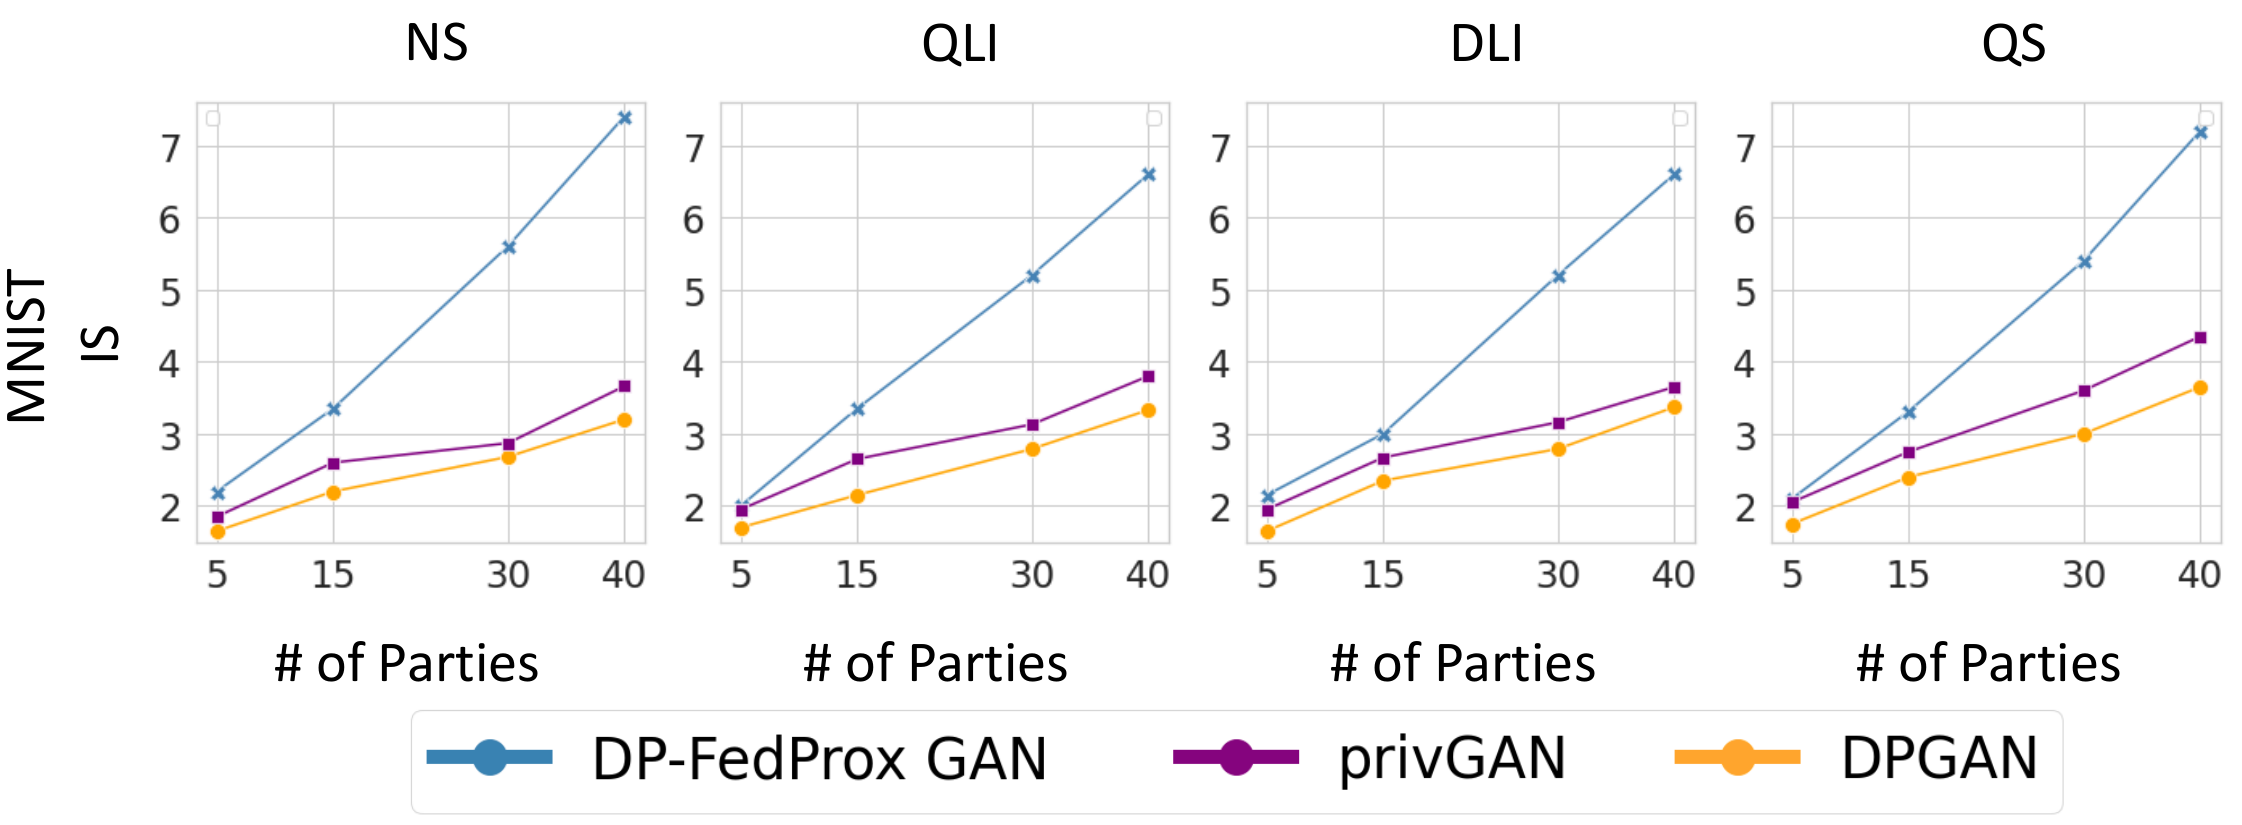
\includegraphics[width=0.96\linewidth]{Plots/vary_parties.png}
	\caption{Varying Number of Parties with MNIST}
 \label{fig:IncreaseClients}
\end{figure}


We investigate the effects of the number of parties ($K$) on utility metrics with the MNIST dataset, as shown in Fig.~\ref{fig:IncreaseClients}. To conduct this experiment, we partition the training set among $K=40$ parties in each distribution setting and select the specified number of parties for model training. We observe higher utility as $K$ increases because private GANs utilize more data contributed by a larger number of parties, which is beneficial for generating high-quality and diversified synthetic data.  DP-FedProx GAN consistently outperforms privGAN and DPGAN, as locally trained GAN models perform poorly due to small amounts of local data.   When larger numbers of parties are involved ($K > 15$),  a significant increase in utility can be observed for DP-FedProx GAN, as opposed to privGAN and DPGAN.  At $K=40$, DP-FedProx GAN achieves around 7 Inception Score while that of privGAN and DPGAN is around 4. It illustrates that the DP-FedProx GAN approach leads to the higher utility when a large number of parties participate. %With privGAN and DPGAN, all distributions have similar utility due to small amounts of local data available for training.  NS with DP-FedProx GAN has better distribution for utility than other non-IID distributions. 





% We investigate the effects of the number of parties $K$ on utility metrics, as shown in Fig.~\ref{fig:IncreaseClients}. To conduct this experiment, we partition the training set in each dataset among $K=40$ parties, according to each distribution.  While we observe lower utility as $K$ increases, we believe the utility loss is directly caused by a reduced local sample size (i.e., more parties with small datasets).  Our future work will improve the simulation such that increasing $K$ would  increase total training data across all parties monotonically.  

% With privGAN and DPGAN, QLI appears to be the better distribution for utility; DP-FedProx GAN performs better in QS than other non-IID distributions.  In CelebA dataset,  privGAN and DPGAN rely on parties with more local data to boost utility measures (better utility in QS settings); DP-FedProx GAN does not incur significant utility loss when increasing the number of parties, as opposed to local private GANs.   It shows that the federated approach is suitable with a large number of parties each having a small set of samples, which is not surprising.  



%  We investigate the effects of the number of parties $K$ on utility metrics, as shown in Fig.~\ref{fig:IncreaseClients}. To conduct this experiment, we partition the training set in each dataset among $K$ parties, according to each distribution.  While we observe lower utility as $K$ increases, we believe the utility loss is directly caused by a reduced local sample size (i.e., more parties with small datasets).  Our future work will improve the simulation such that increasing $K$ would  increase total training data across all parties monotonically.  

% With privGAN and DPGAN, QLI appears to be the better distribution for utility; DP-FedProx GAN performs better in QS than other non-IID distributions.  In CelebA dataset,  privGAN and DPGAN rely on parties with more local data to boost utility measures (better utility in QS settings); DP-FedProx GAN does not incur significant utility loss when increasing the number of parties, as opposed to local private GANs.   It shows that the federated approach is suitable with a large number of parties each having a small set of samples, which is not surprising.  


 
 %Here, we assume that the total amount of data remains fixed when we vary $K$. In training GANs locally, when we distribute data among a larger number of parties, each party suffers due to less data available to train the local model. However, usually, DP-FedProx GAN does not vary much by varying parties in terms of IS. 




%When local parties have QLI and DLI in MNIST, f-MNIST, and CIFAR-10, privGAN provides more diversified and less ambiguous data than DPGAN and DP-FedProx GAN. DP-FedProx GAN, on the other hand, outperforms DPGAN and privGAN across all distributions significantly in terms of IS in CelebA. For example, there is a considerable IS difference of 15.75 between DP-FedProx GAN and DPGAN at K=20 with QLI. Moreover, DP-FedProx GAN has high utility than private GANs trained locally in QS. As local data size varies and labels are assigned randomly in QS, for each round of DP-FedProx GAN, local updates may not deviate much from the global model if they have enough data to train. 



% \begin{figure*}[!h]
% \centering
% \hfill\includegraphics[width=1\textwidth]{Plots/varyClientsSkew.png}\hspace*{\fill}
% 	\caption{\small Varying the Number of Parties with Skew Distribution \textcolor{red}{perhaps we could move all FID figures to supplementary so this figure occupies only a single column}}
% \label{fig:IncreaseClients}
% \end{figure*}




 % We investigate the number of parties' \K effect on utility metrics in private data synthesis from decentralized non-IID data. In private GANs, increasing \K lead to low IS and FID score. In Fig. \ref{fig:IncreaseClients} and \ref{fig:varyClientsNonSkew} shows that when we increase the number of parties \P, IS decreases and FID increases monotonically. When we distribute a fixed amount of data among a larger number of parties in privGAN and DPGAN(applied locally), each party has to train their own local GAN model independently. However, learning the local data distribution effectively with a small amount of data is challenging for a local party. The NS distribution with privGAN and DPGAN has the lowest utility. DP-FedProx GAN with NS, on the other hand, consistently outperforms other private GANs applied locally in terms of utility across all datasets examined. In MNIST, NS exhibits a substantial IS difference of 14.90 between DP-FedProx GAN and DPGAN in CelebA at K=10. 



 
 % When local parties have QLI and DLI in MNIST, f-MNIST, and CIFAR-10, privGAN provides more diversified and less ambiguous data than DPGAN and DP-FedProx GAN. DP-FedProx GAN, on the other hand, outperforms DPGAN and privGAN in QLI and DLI across all parties when the dataset is complicated and small, i.e., CelebA. For example, there is a considerable FID difference of 180.43 between DP-FedProx GAN and privGAN at K=20 with DLI in CelebA in Fig. \ref{fig:IncreaseClients}. With the QS distribution of parties in DP-FedProx GAN, if randomly picked parties have more data, then local parties will contribute more to the global model by updating locally for some steps. For larger numbers of parties, e.g., P>=10, IS and FID has a considerable difference between DP-FedProx GAN and privGAN in QS, as seen in Fig. \ref{fig:IncreaseClients}. 
 
 
 
 % For MNIST, DPGAN utility metrics (i.e., IS and FID) is not significantly decreasing by increasing the number of parties across all distributions. When the number of parties is varied, usually DP-FedProx GAN does not vary much across different distributions compared to privGAN and DPGAN in terms of IS. However, we see some DP-FedProx GAN utility performance degrades more than expected when we increase the number of parties with $\epsilon=$64.11. 
 
 
 % For MNIST, DPGAN utility metrics (i.e., IS and FID) is not significantly decreasing by increasing the number of parties across all distributions. When the number of parties is varied, usually DP-FedProx GAN does not vary much across different distributions compared to privGAN and DPGAN in terms of IS. However, we see some DP-FedProx GAN utility performance degrades more than expected when we increase the number of parties with $\epsilon=$64.11. For example, increasing the number of parties from 5 to 20 reduces DP-FedProx GAN IS by 1.26 in MNIST. As we're accumulating and perturbing more party updates, DP-FedProx GAN requires more privacy budget to converge the GAN model with a larger number of parties. To that end, we increase the privacy budget in DP-FedProx GAN in Fig. \ref{fig:varyParty_DPFedProxGANBudget} to see whether it is still decreasing significantly. However, we observe that we don't see slight variations after increasing the privacy budget $\epsilon$. 


\subsection{Varying Concentration Parameter for Skew Distribution}
\begin{figure}[t]
 \centering
 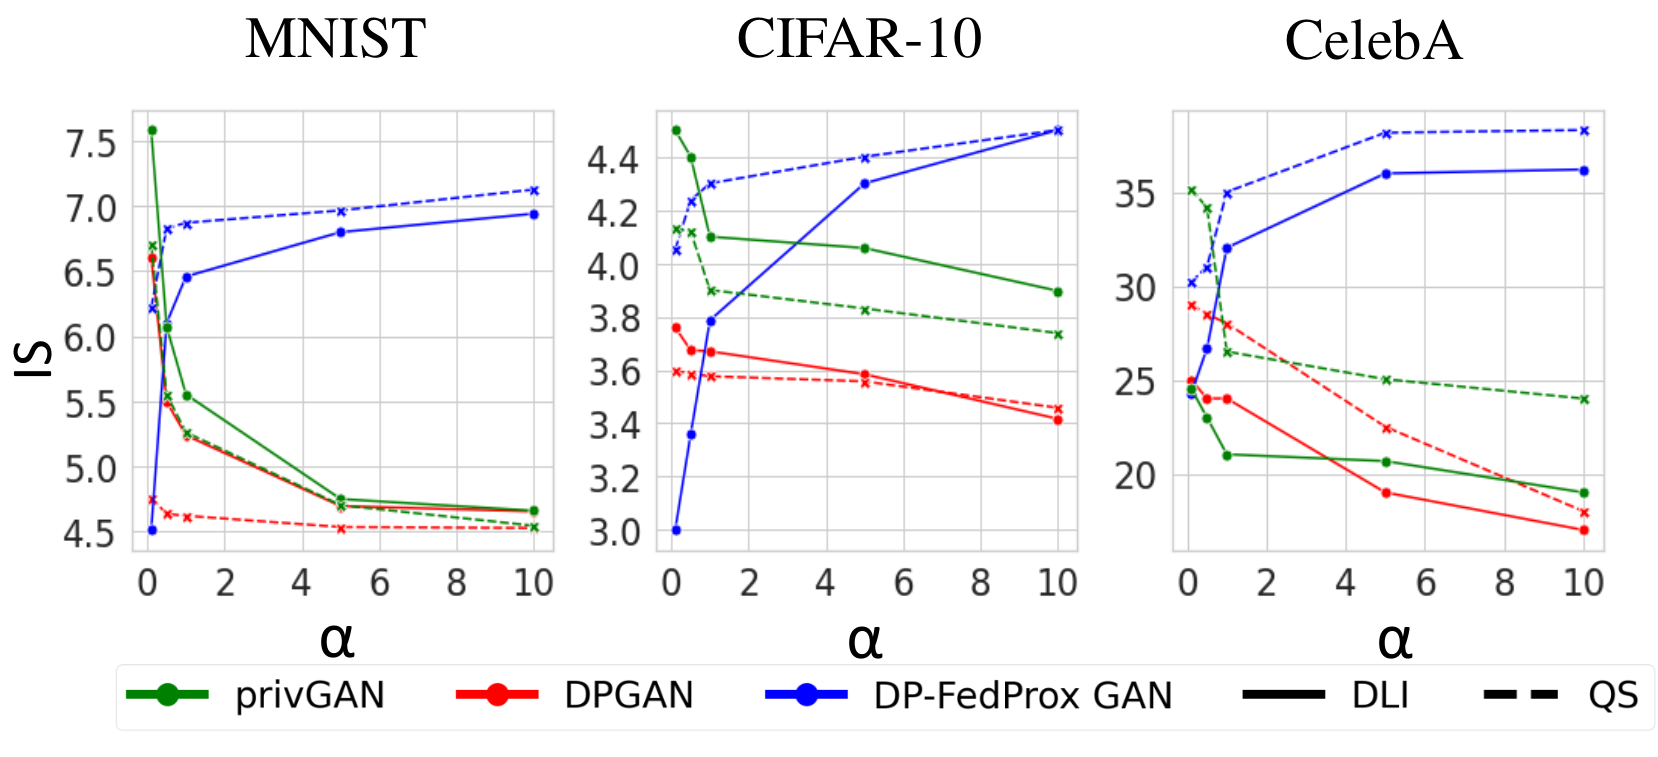
\includegraphics[width=0.95\linewidth]{Plots/varyAlpha.png}
 \caption{Varying Concentration Parameter}
 \label{fig:varyAlpha}
\end{figure}

In this experiment, we investigate how private data synthesis solutions behave by varying the concentration parameter $\alpha$ in Fig. \ref{fig:varyAlpha}. Recall that smaller $\alpha$ values lead to more unbalanced distributions. As we increase the $\alpha$, the data distributions approach the NS setting; as a result, utility drops for privGAN and DPGAN and increases for DP-FedProx GAN.   This result is consistent with our observations early on.   %However,  in DP-FedProx GAN because only a few parties are selected at each round, and if those parties don't have data, it brings instability in GANs training.

When data is highly imbalanced, i.e., low $\alpha$ values, locally trained GANs perform better in DLI than in QS.  The reason is that highly imbalanced label distributions lead to samples from fewer classes at each party, which resembles the QLI setting.  From our observations early on, we know that privGAN and DPGAN perform best in the QLI setting.   As $\alpha$ increases, the difference between DLI and QS diminishes, so does the performance gap between those settings for privGAN and DPGAN.   With lower $\alpha$ values, DP-FedProx GAN performs better in QS than in DLI, as each party in QS settings has a balanced label distribution, which is more helpful for the federated solution.  

% At a smaller $\alpha$ value, QS has a higher utility than DLI in the federated solution. For instance, at $\alpha=0.1$, QS and DLI have an FID difference of 49.32 with DP-FedProx GAN in CIFAR-10. DP-FedProx GAN prefers randomly assigned label data, i.e., QS, so local party updates are closer to the global model than a significant fraction of each label allocated to only a few parties, i.e., DLI. 


 %At $\alpha=0.1$, privGAN and DPGAN have the highest utility. This is because a few parties have data. Ultimately, these parties effectively learn the local party data distribution and contribute more to the global synthetic dataset at the central server. If the party's distribution is more balanced, then DP-FedProx GAN gives high utility performance than privGAN and DPGAN. Similarly, DP-FedProx GAN has similar utility at larger $\alpha$ values i.e, $\alpha \ge $ 5. Furthermore, increasing $\alpha$ beyond a certain value may have similar utility in GANs because distributions are getting similar to each other. 






 
 % In this experiment, we investigate how different private data synthesis solutions behave by varying the concentration parameter $\alpha$ in Fig. \ref{fig:varyAlpha}. With a smaller $\alpha$ value, the partition is more unbalanced. As we increase the $\alpha$, IS decreases, and FID score increases. However, this trend is the opposite in DP-FedProx GAN. QS distribution exhibits a higher IS and lower FID than the DLI in DP-FedProx GAN for all datasets investigated in Fig. \ref{fig:varyAlpha}. When a party's distribution is highly skewed, DP-FedProx GAN has a considerable difference between QS and DLI and shrinks when the $\alpha$ increases.




 
 % For GANs, having randomly assigned labels with a large number of samples for a few parties, i.e., QS is preferable than having a significant fraction of particular labels allocated to only a few parties i.e. DLI . For instance, at $\alpha=0.1$, QS and DLI have a difference of 49.32 IN FID in CIFAR-10. Moreover, when there is enough data with uniformly assigned labels, local parties' GANs in DP-FedProx GAN will not diverge substantially from the global model. We observe that smaller $\alpha$ values, such as 0.1, DP-FedProx GAN, performs poorly, but as the probability of having data for each party increases, thus do the utility increases. 
 



 
 % At $\alpha=0.1$, privGAN and DPGAN have the highest IS and lowest FID for all datasets studied, whereas DP-FedProx GAN has the lowest utility performance. This is because when just a few parties have a significant number of samples, private GANs are applied locally to learn the local party data distribution effectively, and these parties contribute more to the total synthetic dataset at the central server. By increasing the $\alpha$, the local parties distribution is getting more balanced, so in each round in DP-FedProx GAN, randomly selected parties will have a high probability of having enough data to learn the global GAN model locally. If the party's distribution is more balanced, then DP-FedProx GAN gives high utility performance than privGAN and DPGAN. For example, at $\alpha >=5 $, DP-FedProx GAN has IS and low FID scores in MNIST, f-MNIST, CIFAR-10, and CelebA. We notice that CelebA has considerably higher IS and lower FID overall than privGAN and DPGAN e.g. at $\alpha$0 =1, DP-FedProx GAN and DPGAN have a IS difference of 26.24 in CelebA.
 
  
 

%\subsection{Comparison of privacy loss under attacks}

%\textcolor{red}{move 2 out 3 attacks to supplementary}\textcolor{red}{Done. Moved MC Attack and TVD attacks}

%In this section, we vary the privacy parameters to observe their effect on adversary attacks on discriminator. 


\subsection{Membership Inference Attacks}



\begin{table}[]
\centering
\begin{tabular}{|c|c|c|c|c|}
\hline
                                                                                &     & WB    & MC   & TVD   \\ \hline
\begin{tabular}[c]{@{}c@{}}Centralized  GAN\\ ($K=1$)\end{tabular}                  & -  & 48.1  & 77.1 & 0.438 \\ \hline
\multirow{4}{*}{\begin{tabular}[c]{@{}c@{}}Local GANs\\ ($K=10$)\end{tabular}}    & NS  & 11.50 & 68.8 & 0.37  \\ \cline{2-5} 
                                                                                & QLI & 25.10 & 72.1 & 0.45  \\ \cline{2-5} 
                                                                                & DLI & 17.50 & 69.3 & 0.41  \\ \cline{2-5} 
                                                                                & QS  & 18.25 & 70.5 & 0.44  \\ \hline
\multirow{4}{*}{\begin{tabular}[c]{@{}c@{}}Federated GAN\\ ($K=10$)\end{tabular}} & NS  & 21.50 & 72.8 & 0.44  \\ \cline{2-5} 
                                                                                & QLI  & 20.00 & 71.1 & 0.41  \\ \cline{2-5} 
                                                                                & DLI & 20.50 & 68.1 & 0.40  \\ \cline{2-5} 
                                                                                & QS  & 21.12 & 72.2 & 0.43  \\ \hline
\end{tabular}
\caption{Attack results on synthetic images generated with non-private centralized private GAN ($K=1$) as well as non-private local GANs and federated GAN model ($K=10$) with MNIST dataset.}
\label{Tab:WB_Centralized_NonIID}
\end{table}


% \textcolor{red}{if possible, could you use \$\$ around all variables, e.g., $K=10$ vs. K=10, in text, tables, and captions? } 


% \begin{table}[]
% \centering
% \begin{tabular}{|c|c|c|c|c|c|}
% \hline
%                                                                                 &     & NS    & QLI   & DLI   & QS    \\ \hline
% \multirow{3}{*}{\begin{tabular}[c]{@{}c@{}}Local GANs\\ ($K=10$)\end{tabular}}    & WB  & 11.50 & 25.10 & 17.50 & 18.25 \\ \cline{2-6} 
%                                                                                 & MC  & 68.8  & 72.1  & 69.3  & 70.5  \\ \cline{2-6} 
%                                                                                 & TVD & 0.37  & 0.45  & 0.41  & 0.44  \\ \hline
% \multirow{3}{*}{\begin{tabular}[c]{@{}c@{}}Federated GAN\\ ($K=10$)\end{tabular}} & WB  & 21.50 & 20.00 & 20.50 & 21.12 \\ \cline{2-6} 
%                                                                                 & MC  & 72.8  & 71.1  & 68.1  & 72.2  \\ \cline{2-6} 
%                                                                                 & TVD & 0.44  & 0.41  & 0.40  & 0.43  \\ \hline
% \end{tabular}

% \end{table}


\begin{figure}
 \centering
 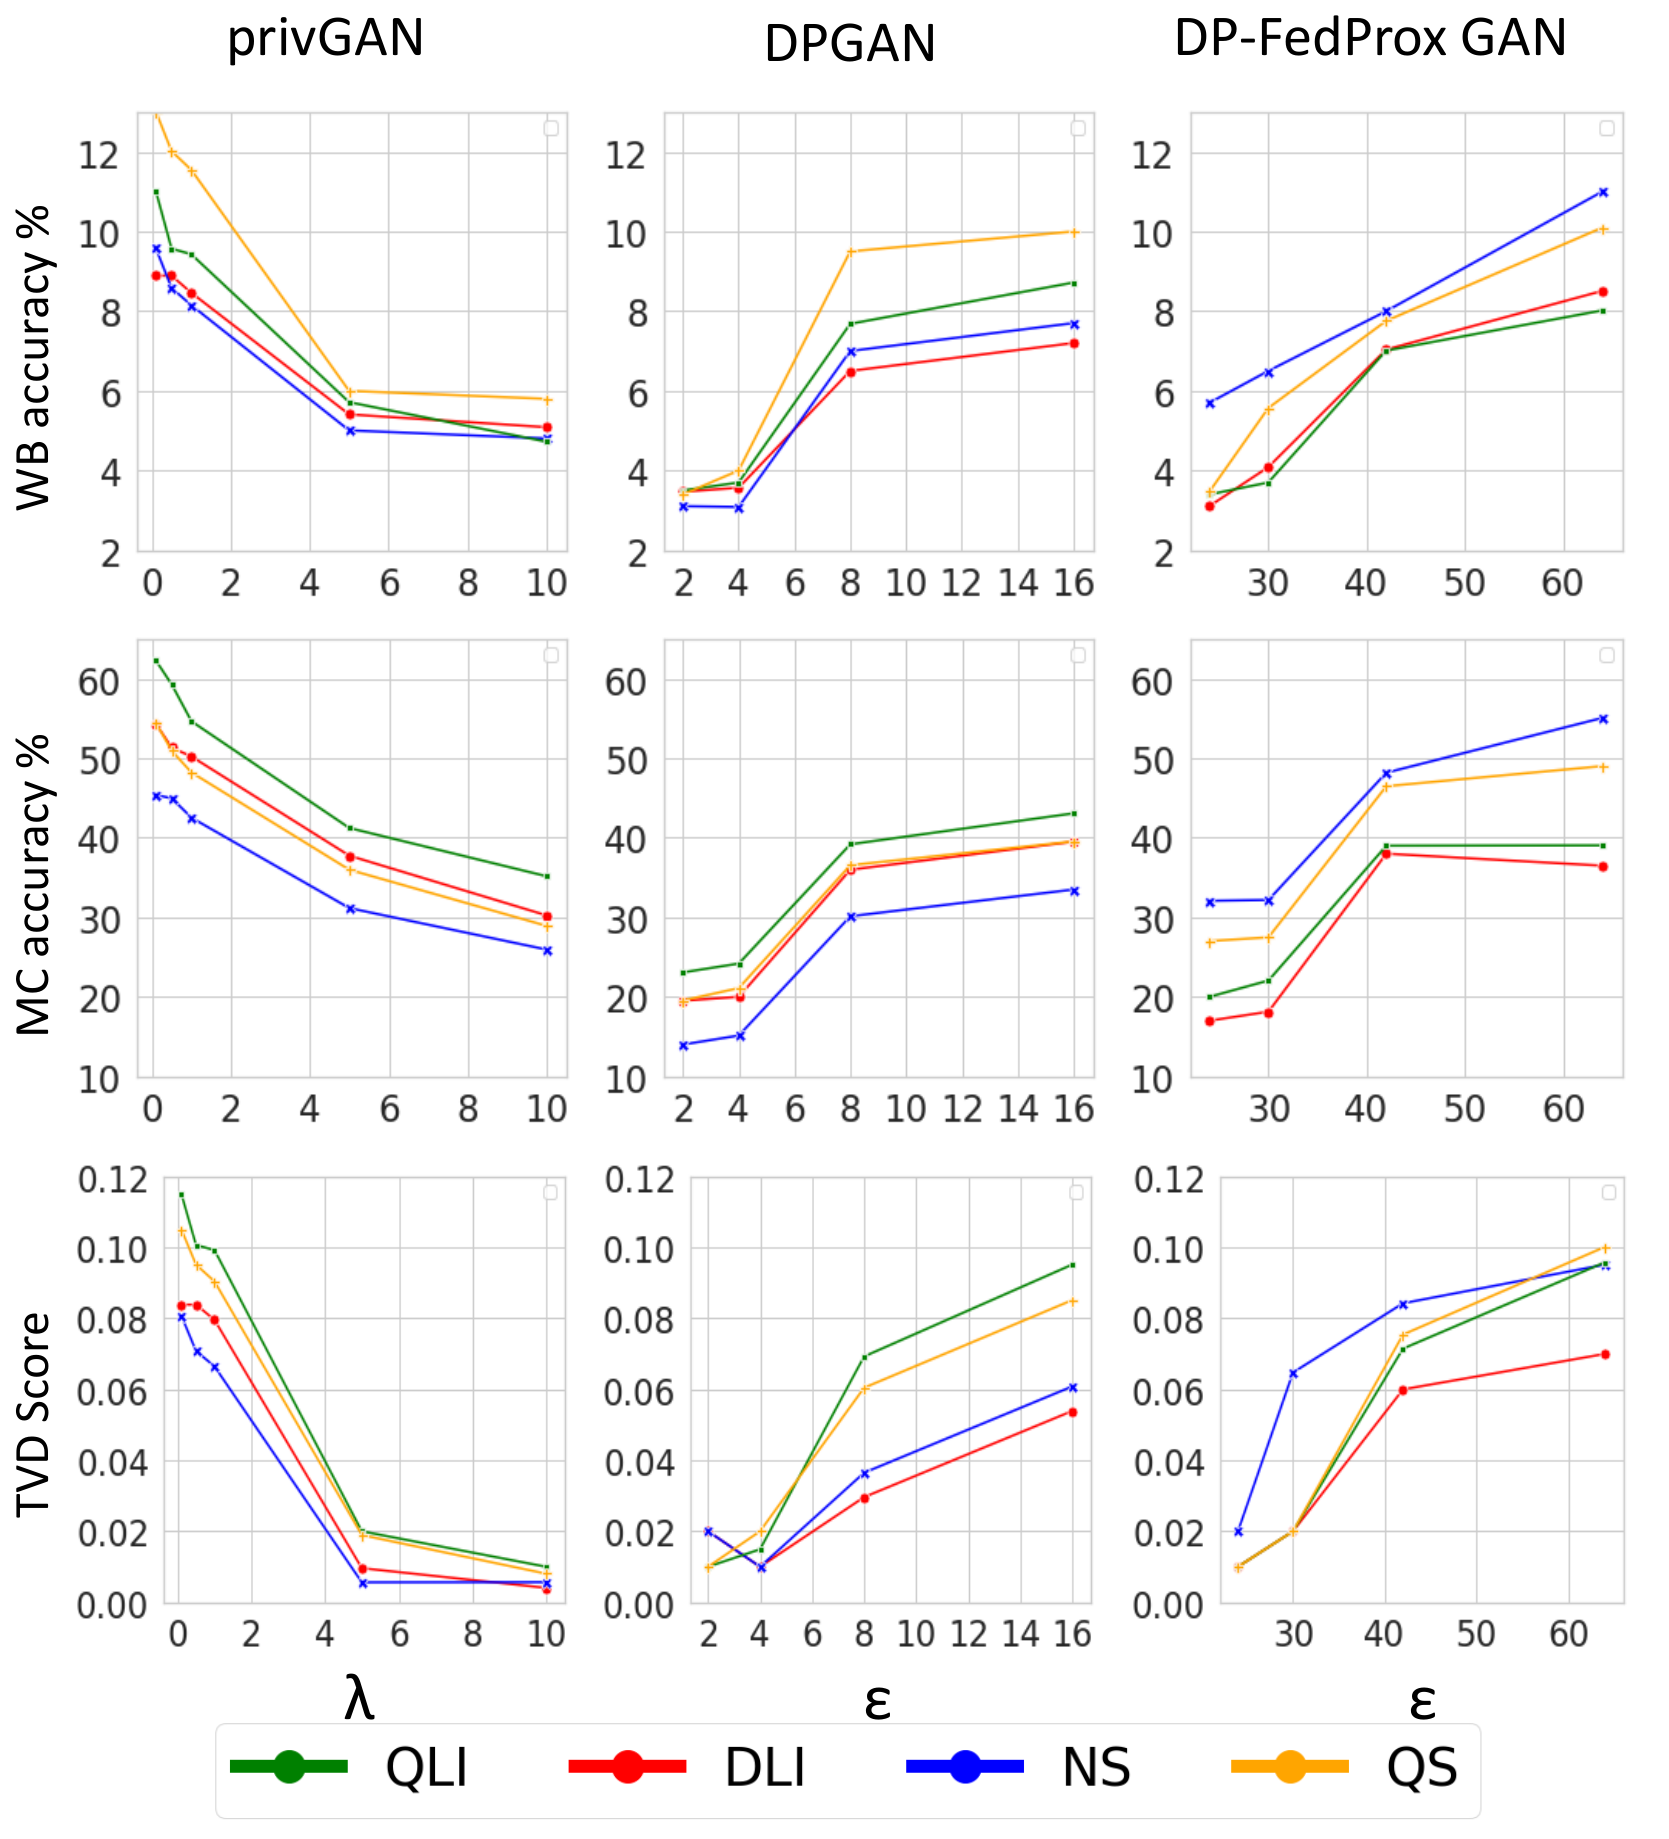
\includegraphics[width=0.9\linewidth]{Plots/vary_privacy_attacks_mnist.png}
 \caption{Attacks on Discriminators and Generators with MNIST }
 \label{fig:varyNoiseWB_MC_TVD}
\end{figure}

In this experiment, we vary the privacy parameters for the private data synthesis solutions to study their defense against membership inference attacks (i.e., WB, MC, and TVD) with the MNIST dataset.  Details regarding the attack implementations can be found in the appendix.    { As a reference, in Table~\ref{Tab:WB_Centralized_NonIID} we present the attack results for non-private centralized GAN as well as local and federated GAN models. In decentralized settings, we observe consistent reductions in the accuracy of WB and MC attacks compared to the centralized setting, but increased TVD scores in some distributions. } 


In Fig.~\ref{fig:varyNoiseWB_MC_TVD}, we report the attack accuracies for private solutions by varying $\lambda$ in privGAN and $\epsilon$ in DPGAN and DP-FedProx GAN.  We observe that private solutions reduce the accuracy of WB, MC, and TVD attacks consistently, with respect to their non-private baselines in decentralized settings.  Furthermore, as we improve the privacy protection, i.e., increasing $\lambda$ in privGAN and decreasing $\epsilon$ in DPGAN and DP-FedProx GAN, the attack accuracies can be further reduced.  

%when we increase $\lambda$ in privGAN and decrease $\epsilon$ in DPGAN and DP-FedProx GAN, the accuracy of attacks decreases.

For locally trained private GANs (privGAN and DPGAN), privacy attacks in the NS setting may be the least successful, compared to non-IID settings.  The lower privacy risk corresponds to the lower utility for privGAN and DPGAN in NS as in Fig.~\ref{fig:varyNoise}, as private local GAN models struggle to learn from small local data.  However, in DP-FedProx GAN, the NS distribution is among the most susceptible to membership attacks, as the federated GAN model learns data distributions well from all parties. 

In the QLI setting, as privGAN and DPGAN perform relatively well in utility (see Fig.~\ref{fig:varyNoise}), the learned generators and discriminators are more prone to membership inference attacks, e.g., higher MC and TVD scores in Fig.~\ref{fig:varyNoiseWB_MC_TVD}.  We also observe that the privGAN and DPGAN discriminators learned in the QS setting can leak membership information, i.e., resulting in higher WB accuracy than other settings, despite lower utility in data synthesis.  On the other hand, in DP-FedProx GAN, the learned discriminator and generator are consistent in privacy leakage among all distribution settings.  Furthermore, the privacy leakage is also consistent with DP-FedProx GAN utility results among all distribution settings.  In the next subsection, we further examine the trade-off between empirical privacy and utility for all private solutions.



%In privGAN, NS distribution-based parties have the lowest privacy risk against membership attacks since none of the local parties have enough data to memorize the underlying distribution. However, in DP-FedProx GAN, NS distribution makes it more susceptible to membership attacks as data distributions are learned from all parties uniformly.

%In terms of the WB attack on discriminators, the results show that private GANs trained locally with QS distribution pose more privacy risk as their discriminators may have more knowledge about the data distribution, making it easier to distinguish between training examples and adversary-controlled data. QS distribution was found to have the highest WB success rate in privGAN and DPGAN.

%As previously noted, in the QLI scenario, the synthetic data generated by privGAN and DPGAN are found to more closely resemble the real data distribution, making them more vulnerable to TVD and MC attacks. However, the outcome of membership attacks on these generators may vary based on the complexity of the dataset used to generate synthetic data with private GANs.


%Our findings show that DP solutions, such as DP-FedProx GAN and DPGAN, have a lower risk of privacy issues, even when using a larger privacy budget ($\epsilon$).  We also found that in DP-FedProx GAN, the models trained with different distributions have similar levels of privacy risk. This indicates that DP-FedProx GAN effectively mitigates the impact of non-IID data.







% \textcolor{red}{For private GANs trained locally, the chance of WB attack  increases for those parties with more data, i.e., QS distribution. Ultimately, those parties' discriminators may have more information about the underlying data distribution to discriminate training examples from other adversary-possessed data. For example, QS has the highest WB attack success in privGAN and DPGAN. On the other hand, other distributions (i.e., DLI, QLI, and NS) generally have similar privacy risks. However, for TVD attacks, we don't observe large attack score differences across various distributions on MNIST.}


% \textcolor{red}{For QLI distribution-based parties, we observed that locally trained GANs' generators have high-quality data, so the chances of a set membership inference attack, i.e., MC, increase for parties with fewer classes to learn. In privGAN, QLI has the highest MC attack accuracy. In DP-FedProx GAN, NS distribution is more vulnerable to various attacks due to learning data distributions uniformly. However, these attack results may change as the complexity of the dataset for the GAN problem changes.  }

% \textcolor{red}{We observe that DP solutions, i.e., DP-FedProx GAN and DPGAN, are less prone to privacy risks even with a larger privacy budget $\epsilon$. In DP-FedProx GAN, we observe that models learned with different distributions have similar privacy risks. It again shows that DP-FedProx GAN is successful in managing the effects of non-IID data.
% }



% In this experiment, we vary the privacy parameters for the private data synthesis
% solutions, to study their defense against membership inference attacks (i.e., WB, MC, and TVD) with the MNIST dataset. \textcolor{red}{ In Table~\ref{Tab:WB_Centralized_NonIID}, we also show the attack results for non-private centralized GAN as well as locals GAN and federated GAN models. } In Fig. \ref{fig:varyNoiseWB_MC_TVD}, when we increase $\lambda$ in privGAN and decrease $\epsilon$ in DPGAN and DP-FedProx GAN, the accuracy of all attacks decreases monotonically.


% \textcolor{blue}{the following paragraph does not seem accurate, especially ``For example, QS has the highest attack success in privGAN and DPGAN".  It does not seem so in Figure 7.}
% \textcolor{red}{For private GANs trained locally, the chance of WB attack  increases for those parties with more data, i.e., QS distribution. Ultimately, those parties' discriminators may have more information about the underlying data distribution to discriminate training examples from other adversary-possessed data. For example, QS has the highest WB attack success in privGAN and DPGAN. On the other hand, other distributions (i.e., DLI, QLI, and NS) generally have similar privacy risks. However, for TVD attacks, we don't observe large attack score differences across various distributions on MNIST.}


% \textcolor{red}{For QLI distribution-based parties, we observed that locally trained GANs' generators have high-quality data, so the chances of a set membership inference attack, i.e., MC, increase for parties with fewer classes to learn. In privGAN, QLI has the highest MC attack accuracy. In DP-FedProx GAN, NS distribution is more vulnerable to various attacks due to learning data distributions uniformly. However, these attack results may change as the complexity of the dataset for the GAN problem changes.  }

% \textcolor{red}{We observe that DP solutions, i.e., DP-FedProx GAN and DPGAN, are less prone to privacy risks even with a larger privacy budget $\epsilon$. In DP-FedProx GAN, we observe that models learned with different distributions have similar privacy risks. It again shows that DP-FedProx GAN is successful in managing the effects of non-IID data.
% }




%As described earlier, this experiment showcases the efficacy of private GANs against a practical adversary who utilizes some proportion of original training data and a GAN model to carry out membership inference attacks. 

% The white box (WB) attack showcases the efficacy of private GANs against membership inference by a practical adversary. We vary the privacy parameters to study their impacts on WB attack results. In Fig. \ref{fig:varyNoiseWB_MC_TVD}, when we increase $\lambda$ in privGAN or decrease $\epsilon$ in DPGAN and DP-FedProx GAN, the attack success decreases monotonically. For private GANs trained locally, the chances of a membership attack increase for those parties with more data, i.e., QS distribution. Ultimately, those parties' discriminators may have more information about the underlying data distribution to discriminate training examples from other adversary-possessed data. For example, QS has the highest WB accuracy in privGAN and DPGAN. On the other hand, other distributions (i.e., DLI, QLI, and NS) generally have similar privacy risks.


%  We also note that datasets with RGB images, such as CIFAR-10 and CelebA, are more susceptible to WB attacks at smaller $\lambda$ values in privGAN. It may be caused by more information retained in GANs model. DP solutions, i.e., DP-FedProx GAN and DPGAN, are less prone to privacy risks even with a larger privacy budget $\epsilon$. In DP-FedProx GAN, we observe that models learned with different distributions have similar privacy risks. It again shows that DP-FedProx GAN is successful in managing the effects of non-IID data. 


% (\textcolor{red}{I'm not sure what you are trying to say here. Does the attack increase for a few parties with more data or majority of parties with less data because of over-fitting?}) (\textcolor{red}{See now})


% Although privacy risk is not changing by large in DP-FedProx GAN across different distributions, QS has a little bit high WB accuracy in CIFAR-10 and CelebA. 

% As shown in Fig. \ref{fig:varyNoiseWB_MC_TVD}, the privacy risk differs between QS and other distributions in stronger privacy settings in privGAN, i.e., $\lambda$0.1 to 1, and DPGAN $\epsilon=$4.01 to 2.1. \textcolor{red}{the difference between QS and others is not large for DPGAN $\epsilon=$4.01 to 2.1. You need to double-check what you meant for DPGAN. } Although privacy risk is not changing by large in DP-FedProx GAN across different distributions, QS has a little bit high score in CIFAR-10 and CelebA. In MNIST, NS has the highest WB attack score across all $\epsilon$ values in DP-FedProx GAN. On the other hand, NS has the lowest vulnerability to attacks in privGAN and DPGAN. At larger $\lambda$ in privGAN and smaller $\epsilon$ in DPGAN, different distributions WB attack score doesn't change much significantly. 
% At higher privacy levels in privGAN and DPGAN, the privacy risk is changing, as shown in Fig. \ref{fig:varyNoiseWB_MC_TVD}. For instance, $\lambda=$5 to 10 in privGAN and $\epsilon=$4 to 2 in DPGAN results in a change of more than 1\% in MNIST, f-MNIST, and CIFAR-10. Results of TVD and MC attacks can be found in supplementary material. 


% As shown in Fig. \ref{fig:varyNoiseWB_MC_TVD}, the privacy risk differs between QS and other distributions in stronger privacy settings in privGAN, i.e., $\lambda$0.1 to 1, and DPGAN $\epsilon=$4.01 to 2.1. \textcolor{red}{the difference between QS and others is not large for DPGAN $\epsilon=$4.01 to 2.1. You need to double-check what you meant for DPGAN. } Although privacy risk is not changing by large in DP-FedProx GAN across different distributions, QS has a little bit high score in CIFAR-10 and CelebA. In MNIST, NS has the highest WB attack score across all $\epsilon$ values in DP-FedProx GAN. On the other hand, NS has the lowest vulnerability to attacks in privGAN and DPGAN. At larger $\lambda$ in privGAN and smaller $\epsilon$ in DPGAN, different distributions WB attack score doesn't change much significantly. 
% At higher privacy levels in privGAN and DPGAN, the privacy risk is changing, as shown in Fig. \ref{fig:varyNoiseWB_MC_TVD}. For instance, $\lambda=$5 to 10 in privGAN and $\epsilon=$4 to 2 in DPGAN results in a change of more than 1\% in MNIST, f-MNIST, and CIFAR-10. Results of TVD and MC attacks can be found in supplementary material. 

% \textcolor{red}{In these two paragraphs above, the writing jumps from QS in privGAN and DPGAN, to DP-FedProx GAN, to privGAN and DPGAN for different datasets. It's random and hard to follow. There should be an underlying logic that determines what you discuss in which order. }


% \textcolor{red}{In addition, you just described what people can read off of the charts by themselves, without offering much insights/hypothesis on why. I suggest the writing should contain 50\% summary of results plus 50\% possible explanations and hypothesis. }


\subsection{Privacy vs. Utility}

\begin{figure}[t]
 \centering
 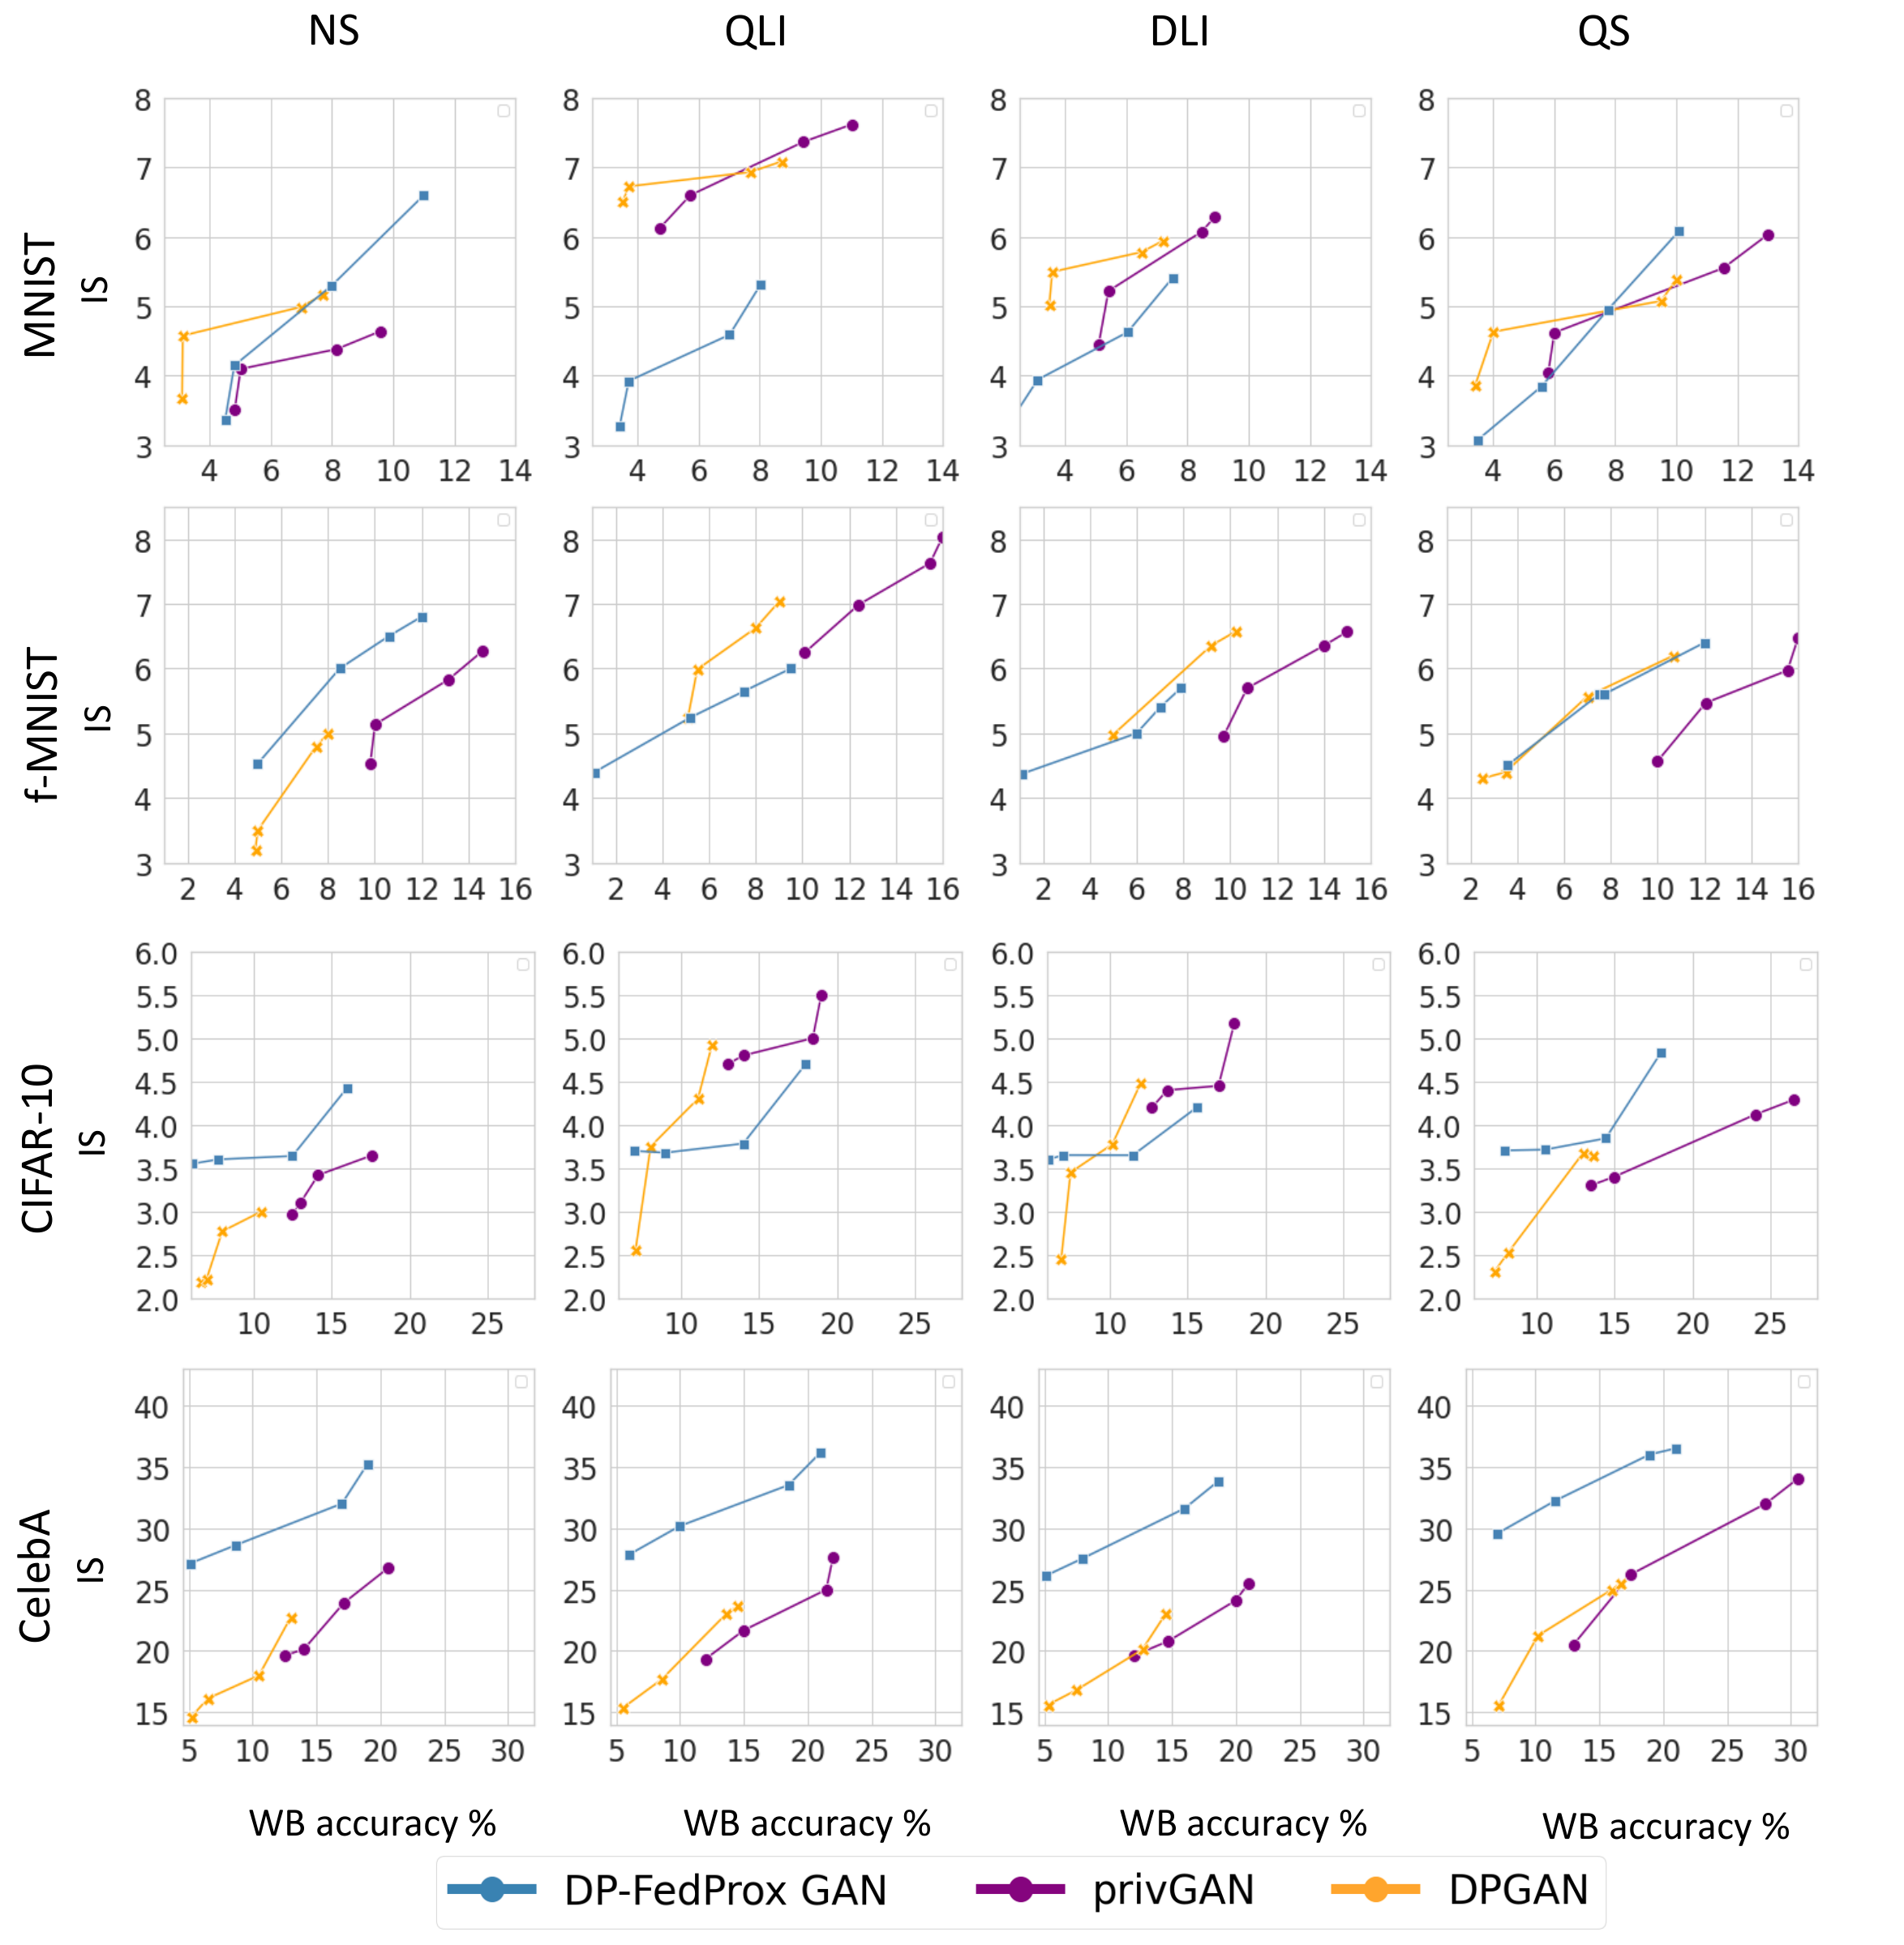
\includegraphics[width=0.98\linewidth]{Plots/wbattackVSis.png}
 \caption{Privacy vs. Utility Tradeoff}
 \label{fig:wbattackVSIS}
\end{figure}

We note that the proposed data synthesis solutions do not share the privacy notion. Specifically, privGAN doesn't provide any privacy guarantees, while DPGAN and DP-FedProx GAN provide record-level and user-level differential privacy guarantees, respectively. Therefore, we conduct a privacy utility trade-off analysis among those solutions in terms of  WB membership inference risks in Fig. \ref{fig:wbattackVSIS}.  It can be observed that generally privGAN results in higher WB attack risks than DPGAN and DP-FedProx GAN.  


% The tradeoff analyses for MC and TVD risks can be found in the online appendix.

%We also notice that at lower similar WB accuracy, DP-FedProx GAN has more utility than DPGAN. 

We observe that DP-FedProx GAN the best privacy-utility tradeoff in NS distributions: given a WB accuracy, DP-FedProx GAN often provides better IS scores than privGAN and DPGAN.   DPGAN provides good privacy-utility tradeoff in non-IID distributions for three simpler datasets (i.e., MNIST, f-MNIST, CIFAR-10).  In non-IID distributions for those datasets, privGAN may provide better utility at the expense of increased privacy risks.   

%so it may be helpful for adoption when parties have NS distribution. For example, DP-FedProx GAN generally has a higher utility at similar privacy risks than privGAN. Although in QLI and DLI distribution, generally, privGAN has significantly higher utility than other solutions. Still, at the same time, they are exposed more to white-box attacks.


For the CelebA dataset, DP-FedProx GAN clearly outperforms privGAN and DPGAN, by consistently dominating two other methods in utility at the same privacy risk level.  This shows DP-FedProx GAN is superior in balancing privacy and utility with a large number of classes ($1000$) and few samples per class ($30$).    Both locally trained private GANs suffer from lower utility and privGAN yields higher privacy risks, due to their lack of privacy guarantees.  

%, provides a significantly higher utility with lesser privacy risks. Other solutions applied locally have substantially lower utility with higher privacy risk. 

% s, DP-FedProx GAN has more utility than DPGAN. DP-FedProx GAN has the highest utility with less privacy risk in NS distribution. For example, at similar privacy risks between privGAN and DP-FedProx GAN in NS, DP-FedProx GAN has generally high IS. In QLI and DLI, DPGAN has a bit high utility than DP-FedProx GAN with less exposure to privacy risks, i.e., White-box accuracy, in MNIST, f-MNIST, and CIFAR-10. privGAN has the highest IS and WB accuracy from learning data distribution from QLI and DLI in MNIST, f-MNIST, and CIFAR-10. Although in QLI distribution, private GAN solution applied locally, i.e., privGAN, has significantly higher utility than other solutions. Still, at the same time, they are exposed more to white-box attacks in MNIST, f-MNIST, and CIFAR-10. In CelebA, the federated solution DP-FedProx GAN for private data synthesis, i.e., solution, is working. Moreover, DP-FedProx GAN provides a significantly higher utility with fewer privacy risks. Here, private GANs solutions applied locally have substantially lower utility. DPGAN is less vulnerable to membership inference attacks with lesser utility. 


\section{Discussion}

%In this section, we present the interpretation of our evaluation and discuss practical implications.

\partitle{Interpreting the Results} %Below, we discuss several observations that may help adopt private data synthesis solutions and motivate future research in private data synthesis from decentralized non-IID data. 
Considering the results combined, we note that DP-FedProx GAN outperforms privGAN and DPGAN in non-skew and moderately skewed settings (see Fig.~\ref{fig:varyNoise} and \ref{fig:varyAlpha}). In highly skewed settings, its strong user-level differential privacy may lead to higher utility loss, as parties have equal chance of participating in each round despite the amount of local data. %\textcolor{red}{DP-FedAvg GAN, is unsuitable for learning from highly skewed non-IID distributions}. 
On the other hand, training privGAN or DPGAN locally may yield good utility in non-IID settings, as parties with larger amounts of data dominate the quality measures. Among different non-IID distributions, local privGAN and DPGAN show great promise for QLI, where each party focuses on synthesizing samples of a small number of classes; DP-FedProx GAN produces similar results for all non-IID distributions, demonstrating its capability to learn a variety of data distributions. For complex tasks, e.g., learning the subsampled CelebA with a large number of classes and fewer samples per class, all approaches produce better quality data in QS settings; the difference between  distributions diminishes by increasing the amount of skewness as in Fig.~\ref{fig:varyAlpha}. {Lastly, increasing the number of parties significantly boosts the utility of DP-FedProx GAN, while privGAN and DPGAN only show marginal utility gain as in Fig.~\ref{fig:IncreaseClients}.}



%Firstly, we see whether server-level or local-party-level private data synthesis solutions are effective in terms of utility. In our evaluation, we observe that if only a few %parties have data, i.e., QS, then other parties with less data suffer by not learning the underlying distribution of data using private GANs(DPGAN and privGAN) applied locally (see Fig. \ref{fig:varyNoise} and \ref{fig:IncreaseClients}). Moreover, their samples will have less representation in the global synthetic dataset at untrusted/central server, while these solutions may work for other parties. Overall, private GANs applied locally works only in skew distributions (QLI, DLI, and QS) because parties with larger data dominate the other parties' shortcomings. 

% Although Fig.~\ref{fig:IncreaseClients} shows reduced utility for larger numbers of parties, we emphasize that the reduced quantity of local data and increased skewness are the main factors that lead to those results. 


 %We notice that when local parties have fewer classes to learn, i.e., QLI, local private GANs like privGAN and DPGAN work better than DP-FedProx GAN because having few classes makes the local GAN problem easy (see Fig. \ref{fig:varyNoise}). On the other hand, server-level private synthesis solutions, such as DP-FedProx GAN, ensure that each party has an equal chance of being chosen in each round. This way, parties with a small amount of data also contribute to global private synthetic data (see Fig. \ref{fig:varyClientsNonSkew}). 




\partitle{Deployment Choice} %We recognize that the priorities of private data synthesis solutions from decentralized non-IID data may vary greatly. 
Given different privacy models and wide variability in utility performances, there is no one-size-fits-all solution for private synthesis with decentralized non-IID data. While training GAN models locally provides full autonomy to each party, training federated GAN models allow all parties to contribute meaningfully, even those with very small amounts of local data. Furthermore, DP-FedProx GAN motivates local parties to jointly train models, as it shows significant utility benefits as the number of parties increases in Fig.~\ref{fig:IncreaseClients}.     Moreover, we showcase how to conduct a trade-off analysis between utility measures and empirical privacy risks as in Fig.~\ref{fig:wbattackVSIS}. It can be observed that privGAN may lead to higher privacy risks, due to lack of a formal privacy model. We argue that approaches that provide differential privacy guarantees {(i.e., DPGAN and DP-FedProx GAN)} should be considered due to their rigorous and future-proof privacy protection.  




%For organizations that require provable privacy guarantees, DPGAN and DP-FedProx GAN can be considered as it is based on differential privacy. When providing a record-level DP guarantee is needed, the organization may consider DPGAN, which provides privacy protection to every record of training data. Similarly, when providing a user-level DP guarantee is required, then the organization may consider DP-FedProx GAN, which provides a DP guarantee that applies to all of a user's data rather than just a single training sample. While privGAN does not provide any privacy guarantees similar to differential privacy-based techniques, some certificate of membership privacy can often be required by data/model owners as well as regulators. 

%There is a common observation in white-box membership inference attacks that local parties with more data, i.e., QS, are more vulnerable to these attacks (see Fig. \ref{fig:varyNoiseWB_MC_TVD}, \ref{fig:varyNoiseTVD} and \ref{fig:varyNoiseMC}). Generally, privGAN has the highest utility with the highest privacy risks. Moreover, DPGAN is not effective much in utility but provides stronger privacy protection against membership inference attacks. DP-FedProx GAN, on the other hand, has many advantages that are effective in learning the underlying distribution of decentralized non-IID data with lesser privacy risks. Furthermore, in terms of privacy risk and utility, it does not differ much across different (skew and non-skew) distributions. 

%Based on recent research \cite{DP_GDPR_2019}, differential privacy should be the preferred method for GDPR-compliant systems since it explicitly eliminates memorization and overfitting while still allowing for reliable data analysis tasks. Furthermore, realistic SOTA membership inference attacks against models/synthetic datasets might potentially be used to estimate privacy risk. Recently, \cite{xu2022mace} used a Bayes Optimum Classifier as an optimal adversary and offers a dataset-dependant and query-specific membership privacy loss estimate with confidence intervals. In these attacks, the adversary's performance estimate can serve as a post-doc certificate for models/synthetic datasets due to a powerful adversary. A data/model owner may get such certifications for various queries relevant to their domain to determine the overall vulnerability of the model/synthetic data.

%Moreover, if a local party does not have enough data to train but still desires to generate private data with higher utility and lower privacy risk. In that case, DP-FedProx GAN can be considered there. Similarly, where distributions are very skewed local private GANs solutions like privGAN and DPGAN will not work for a few parties. 

%Usually, GAN models require higher computational power than basic machine learning models such as regression machine learning models. For businesses unable to train models locally owing to computing power constraints, DP-FedProx GAN is a better option since all stakeholders collaborate to train the global model privately. More details about communication and computation complexity are discussed in the supplementary material.



\partitle{Practical Considerations} Needless to say, a number of considerations should be addressed for the practical adoption of the proposed solutions. Firstly, all parties must agree on the training mode (i.e., local vs. federated) and the privacy settings (e.g., $\lambda$ and $\epsilon$). When parties have different privacy requirements (e.g., in terms of $\epsilon$ values for DP), the strongest privacy level (e.g., lowest $\epsilon$) should be adopted to ensure privacy for all parties. Secondly, in the local GAN training approach, when each party contributes synthetic data of the same size as that of the local dataset, it may disclose aggregate-level information about private data.  That may be addressed by applying differential privacy (e.g., Laplace mechanism~\cite{dwork_book}) to the local count and sampling synthetic records according to the noise count. Lastly, we recommend grid search approaches for uncovering suitable hyper-parameters in local training approaches and weight-sharing for the federated GAN training. Recent research on hyper-parameter optimization in federated settings~\cite{khodak2021federated} may provide new opportunities for the practical deployment of the federated approach.  











%When generating private data from decentralized non-IID data, we must consider a number of factors. 


%In our experiments, utility is evaluated at the central server, assuming that each local party reports synthetic data equivalent to the amount of their local data in privGAN and DPGAN. On the contrary, evaluating utility at the central server may be challenging if local parties report random amounts of synthetic data without disclosing their local data size. 


%\textcolor{red}{discuss points should be based on the results of our study, i.e., utility/privacy/tradeoff for the synthetic data.}\textcolor{red}{Done}

%If most parties have a small amount of data or the dataset is complex in decentralized scenarios, it is recommendable to choose federated solution i.e DP-FedProx GAN for private data synthesis. Based on our observation, DP-FedProx GAN is more consistent in generating high-quality and more diversified images in different skew distributions while less prone to adversarial attacks.


%However, we observe that if $\alpha$ value is very small $\alpa$ =0.1 in QS, then DP-FedProx GAN is not recommendable because only few parties will have data to train and other parties will have very few samples. On the other hand, if we train privGAN and DPGAN locally with QS distribution with $\alpa$ =0.1 then local parties with more data are more vulnerable to adversary attacks.


%As previously stated, we assume that each local party reports synthetic data equal to the amount of local data in the privGAN and DPGAN cases. From an adversary perspective, it may leak private information about local data size and lead to a successful white-box attack \cite{WBAttack2018}. On the other hand, we recommend that local parties should report \n generated samples to a central server where \n is a differential-private count number. Here, \n can be generated by DP Google's Rappor mechanism \cite{Erlingsson_2014} or DP Laplace mechanism \cite{HolohanLaplace2018}. \textcolor{red}{this mechanism will work for single count release?}

%In the case of privGAN, where we have multiple generators for each local party, each may result in a slightly different generated data distribution. Hence, it is recommendable to generate data from both of these generators before sharing it with the central party. Similarly, we encourage more parties to share private synthetic data because it increases the diversity of shared data. 


 %We recommend conducting a grid search approaches to uncover suitable hyperparameters related to query-specific privacy for practical data/model sharing. Local parties should be able to identify hyperparameters that offer enough privacy protection and utility for their settings. We suggest local parties to modify privacy budget $\epsilon$ in (DPGAN and DP-FedProx GAN), and $\lambda$ in privGAN according to their requirements of privacy and utility. If local parties have smaller amount of data then its not recommendable to use large number of discriminator-generator pairs. 
 


%Furthermore, sharing models for the benefit of reproducible research is recommendable. In the privGAN and DPGAN cases, where multiple local parties are engaged, releasing one or a randomly selected model from local parties might be a good idea instead of all pairs to enhance membership privacy further. We suggest that privacy discriminator $D_p$ in privGAN should not be shared since an adversary's ability to guess which generator generated a certain synthetic sample might be used to infer membership. \textcolor{red}{exclude this paragraph?}

 %\textcolor{red}{is it what we did? talk about recommendations from our experience/results and provide references if any.}\textcolor{red}{Done}




% utility is evaluated at the central server, assuming that each local party reports synthetic data equivalent to the amount of their local data. On the contrary, evaluating utility at the central server may be challenging if local parties report random amounts of synthetic data without disclosing their local data size.



% While the relationship between privacy and synthetic data sharing has been extensively explored, it is still important to find out when it is suitable to share models or only synthetic data. This section will cover some practical issues regarding synthetic data/model sharing in the context of decentralized non-IID data. In a decentralized data case, sharing all local parties' models/share is challenging because sometimes different organizations have different data/model sharing constraints. Multinational corporations, for example, must abide by the laws of the country in which they operate. In this case, some may agree to exchange data/models, while others may not. In the case of decentralized non-IID, consent of local parties is necessary other than data regulation issues.


% When feasible, sharing solely synthetic data is the preferred choice since it enables only black box attacks, which are typically seen as less successful than white box attacks for GANs\cite{WBAttack2018}. In a federated solution, a global generator at the central server can generate and release the date. On the other hand, in other case, we have multiple generations and discriminators where privGAN and DPGAN are applied locally, so we have to release the data from all of generators. 


\section{Conclusion}

In this paper, we studied several practical solutions for private synthesis using GANs with decentralized, non-IID data.
Among them, privGAN and DPGAN can be trained by each party locally and DP-FedProx GAN is trained jointly by all parties with strong user-level differential privacy guarantees. We conducted an extensive empirical evaluation with data from multiple image domains and simulated a variety of non-IID distributions. %We investigated centralized private GAN systems, such as privGAN and DPGAN, and proposed a DP-FedProx GAN, a federated learning solution with stronger privacy for decentralized non-IID data.
We provided an in-depth analysis of the evaluation results, regarding the usefulness of synthetic data, privacy risks in membership inference attacks, and the privacy utility trade-off for the proposed solutions. 

%\textcolor{red}{Need to write two to three future research directions, see my other papers for example. }


Several directions are open for future research on private data synthesis from decentralized non-IID data. Firstly, it is helpful for future research to address data with imbalanced labels. Privacy risks may be higher due to class imbalance \cite{FarrandMST20}. Achieving high data synthesis utility for class-imbalanced data may also be challenging, especially for rare classes.  %Moreover, new privacy challenges may arise when few users have more data or overlap exist for few users among local data sites. 
Secondly, understanding the usefulness of synthetic data in various applications would be beneficial, e.g., in clinical decision support systems. Thirdly, future research may extend to emerging federated learning results for non-IID data, such as FedCurv~\cite{shoham2019overcoming}, which proposes to share additional elements by each local party to overcome forgetting. As a result, such approaches may lead to additional privacy risks and thus demand new solutions.  Lastly, it would be interesting to develop grid search approaches for hyper-parameters in federated GAN training, with privacy guarantees, e.g., differential privacy. It will help provide end-to-end privacy for data synthesis in decentralized settings.  %In the context of new emerging privacy risks, we consider developing new private data synthesis solutions from non-IID data with high utility and stronger privacy protection


\section*{Acknowledgment}
The authors would like to thank the anonymous reviewers for their feedback, which helped improve the manuscript. 

\bibliographystyle{IEEEtran} \balance
\bibliography{references} 
\appendix



\subsection{Implementation Details}

% \subsection{Modeling and optimization}
 % 

For MNIST and f-MNIST, we use standard, fully connected networks for both generators and discriminators. On the other hand, we adopt a Deep Convolutional Generative Adversarial Network (DCGAN) structure for CIFAR-10 and CelebA datasets. All GAN models have identical generator and discriminator architectures for the respective dataset.

% EMNIST \cite{cohen2017emnist}

% \textcolor{blue}{can we report the generator and discriminator architectures for each dataset for reproducibility?}

For evaluation, we train the privGAN models with an Adam ($\beta$=5) optimizer for both generator and discriminator.  For differentially private GANs (i.e., DPGAN, DP-FedProx GAN, and DP-FedAvg GAN), we use Differentially Private Stochastic Gradient Descent (DP-SGD) optimizer for the discriminator. For the generator, we use  Adam ($\beta$=5) optimizer in DPGAN and SGD optimizer in DP-FedProx GAN and DP-FedAvg GAN.  We set a 0.0002 learning rate for all optimizers.  The batch size adopted for privGAN is 256.  For DP-GAN, the batch size is varied from 16 to 64 in order to meet the specified privacy parameter $\epsilon$.  For DP-FedProx GAN and DP-FedAvg GAN, the batch size is set to 32 for CIFAR-10 and CelebA and to 64 for other datasets.  

% The default values used are $\epsilon$=98.01,  and the sampling probability $q$ is 0.1 in DP-FedSGD GAN.

% Learning rates may change with respect to a dataset  and beta values batch size

While evaluating the different adversarial attacks on privGAN, we train privGAN for 500 epochs using the same optimizer and hyperparameters. Similarly, we train all differentially private GAN models with a fixed privacy budget $\epsilon$, setting the noise scale $z$ to achieve the specified $\epsilon$. For WB and TVD attacks, we use 10\% of the training set to train models, following the approach in~\cite{WBAttack2018}.

 
 To evaluate the MC attack, we follow the methodology in ~\cite{PrivGAN2019, MCAttackHilprecht2019}.  We use 10\% of the training set for training the attack model and evaluate the model on the residual 90\% of the training set.  The test set is utilized solely to calculate the principal components for all datasets.  In federated training (i.e.,  DP-FedProx GAN, and DP-FedAvg GAN), the central server generates 100,000 synthetic samples. In local training (i.e., privGAN and DPGAN), we sample 100,000 synthetic samples from each party. %We reported the MC attack results over 10 runs. %Here, the training set was picked at random from 10\% of the dataset for each run. More details about the MC attack can be found in ~\cite{MCAttackHilprecht2019}. 
 
In order to ensure the results are representative, we performed each experiment five times and reported the average outcomes for both utility and adversarial assessments. %Additionally, to simulate non-IID data distribution, we used a different seed each time.

% (\textcolor{red}{in the para above, MC was averaged among 10 runs vs. 5? })
\subsection{Complexity Analysis}

% \textcolor{red}{see my comment on Google spreadsheet for revision.}
% \textcolor{blue}{In the context of locally trained GANs, the time complexity can be expressed as $O(K(DEM))$, with $K$ denoting the number of parties, $D$ representing the dataset subset size per party, $E$ corresponding to epochs, and $M$ encompassing model complexity, which includes the parameters and associated computational cost during updates. On the other hand, the Federated GANs training framework comprises two essential components: local model training and global model aggregation. The complexity of local model training is given by $O(K(DEM))$, and the global model aggregation phase is $O(TM)$, with $T$ signifying the number of communication rounds for global model updates. As a result, the overall time complexity of the federated GANs is approximated as $O(K(DEM) + TM)$. The choice between locally-trained GANs and Federated GANs depends on the specific needs and priorities of the problem. The selection between locally-trained GANs and Federated GANs depends on the specific needs and priorities of the problem. When data privacy is of significant concern, the Federated GANs may be the most appropriate approach, despite having a higher time complexity.
% }

In DP-FedProx GAN and DP-FedAvg GAN, the time complexity for each party is $O(nBT)$, where $n$ represents the number of steps for local discriminator and generator updates, $B$ represents the batch size, and $T$ represents the total number of rounds.  In the context of privGAN and DPGAN, the time complexity for each party can be expressed as $O(|D|E)$, where  $|D|$ is the upper bound of local data size, and $E$ corresponds to the number of epochs for local model training.

%Each party conducts a local discriminator update involving a designated number of discriminator steps ($n$) per round. In each step, gradients for the discriminator are computed based on real and synthetic data batches of size $B$. Thus, the complexity of this stage is expressed as $O(n B )$. Similarly, every party performs a local generator update with a specified number of generator steps ($n$) per round. Here we use the same $n$ for the local generator and discriminator.  In each step, gradients for the generator are calculated using synthetic data batches of size $B$. The complexity of this stage is expressed as $O(n B)$. Consequently, the party-side complexity for the federated GAN  is $O(T(n B))$. 

% Concerning server-side complexity, processes include local updates aggregation, noise addition to the aggregated update, and the global generator update. The server aggregates local updates for the discriminator with complexity $O(K )$, where $K$ is the number of participants and $M_D$ indicates the discriminator's model complexity. Gaussian noise is added to the aggregated update with complexity $O(M_D)$ to ensure privacy. Finally, considering the updated discriminator, the server executes a generator update with complexity $O(n_G B M_G)$. Considering these steps, the federated GAN's server-side complexity is $O(K M_D + M_D + n_G B M_G)$. 




%Choosing between locally-trained GANs and  federated GANs depends on the problem's specific needs and priorities. If data privacy is a critical concern, the federated GAN  may be favored for its privacy-preserving features. However, it is vital to weigh this advantage against the potentially increased time complexity compared to locally-trained GANs.
% \clearpage
% \newpage
% \onecolumn
\appendix


\subsection{Implementation Details}

% \subsection{Modeling and optimization}
 % 

In this section, we outline the modeling details and model architectures. For MNIST and f-MNIST, we use standard, fully connected networks for both generators and discriminators due to the simplicity of datasets. On the other hand, we adopt a Deep Convolutional Generative Adversarial Network (DCGAN) network structure for EMNIST \cite{cohen2017emnist}, CIFAR-10, and CelebA datasets. All GAN models have identical generator and discriminator architectures for the respective dataset (see details below). 

% \textcolor{blue}{can we report the generator and discriminator architectures for each dataset for reproducibility?}

For the utility evaluation, we train the privGAN models with an Adam( $\beta$=5 ) optimizer (for both generator and discriminator), and the batch size is 256. The default values used are $\epsilon$=98.01,  and the sampling probability $q$ is 0.1 in DP-FedSGD GAN. For  differentially private GANs (i.e., local DPGANs, DP-FedProx GAN, DP-FedAvg GAN, and DP-FedSGD GAN), we use Differentially Private Stochastic Gradient Descent (DP-SGD) optimizer for the discriminator. While for the generator, we use  Adam ( $\beta$=5 ) optimizer in DPGAN and SGD optimizer in DP federated GANs (i.e., DP-FedProx GAN, DP-FedAvg GAN, and DP-FedSGD GAN). Moreover, differentially private GANs are trained with the fixed privacy budget $\epsilon$. Here, we used a 0.0002 learning rate for all optimizers.

% Learning rates may change with respect to a dataset  and beta values batch size

 While evaluating the different adversarial attacks on privGAN, we trained privGAN for 500 epochs with the same optimizer and hyper-parameters. Similar to utility evaluation,  all differentially private GAN models are trained with the fixed privacy budget $\epsilon$, and noise scale $z$ is set to achieve the specified $\epsilon$.  For White–box and TVD attacks, 10\% of the data are used to train models, similar to ~\cite{WBAttack2018}.
 
  For the MC attack, we first isolated the test data and utilized it alone to compute the principal components for all datasets as described in ~\cite{PrivGAN2019, MCAttackHilprecht2019}. The remaining 10\% of the dataset was then utilized for training models, with the model being tested on all data except the held-out test data. In federated training (i.e.,  DP-FedProx GAN, DP-FedAvg GAN, and DP-FedSGD GAN), the central server generates 100,000 synthetic samples. While training locally (i.e., privGAN and DPGAN), each party share 100,000 synthetic samples with a central server. We reported the MC attack results over 10 runs. Here, the training set was picked at random from 10\% of the dataset for each run. More details about the MC attack can be found in ~\cite{MCAttackHilprecht2019}. 
 
To make sure the results were accurate, we conducted each experiment 5 times and reported the average numbers. This was done for both utility and adversarial evaluations. Additionally, to simulate non-IID data distribution, we used a different seed each time.




\subsection{Implementation Details}

% \subsection{Modeling and optimization}
 % 

For MNIST and f-MNIST, we use standard, fully connected networks for both generators and discriminators. On the other hand, we adopt a Deep Convolutional Generative Adversarial Network (DCGAN) structure for EMNIST \cite{cohen2017emnist}, CIFAR-10, and CelebA datasets. All GAN models have identical generator and discriminator architectures for the respective dataset (see details below).

% EMNIST \cite{cohen2017emnist}

% \textcolor{blue}{can we report the generator and discriminator architectures for each dataset for reproducibility?}

For evaluation, we train the privGAN models with an Adam ($\beta$=5) optimizer for both generator and discriminator. The default values are $\epsilon$=98.01,  and the sampling probability $q$ is 0.1 in DP-FedSGD GAN. For differentially private GANs (i.e., DPGAN, DP-FedProx GAN, and DP-FedAvg GAN), we use Differentially Private Stochastic Gradient Descent (DP-SGD) optimizer for the discriminator. For the generator, we use  Adam ($\beta$=5) optimizer in DPGAN and SGD optimizer in DP-FedProx GAN, DP-FedAvg GAN, and DP-FedSGD GAN.  We set a 0.0002 learning rate for all optimizers.  The batch size adopted for privGAN is 256.  For DP-GAN, the batch size is varied from 16 to 64 in order to meet the specified privacy parameter $\epsilon$.  For DP-FedProx GAN and DP-FedAvg GAN, the batch size is set to 32 for CIFAR-10 and CelebA and to 64 for other datasets.  


 While evaluating the different adversarial attacks on privGAN, we trained privGAN for 500 epochs with the same optimizer and hyper-parameters. Similarly, all differentially private GAN models are trained with the fixed privacy budget $\epsilon$, and noise scale $z$ is set to achieve the specified $\epsilon$.  For WB and TVD attacks, 10\% of the training set is used to train models, similar to~\cite{WBAttack2018}. 
 
 To evaluate the MC attack, we follow the methodology in ~\cite{PrivGAN2019, MCAttackHilprecht2019}.  We use 10\% of the training set for training the attack model, and evaluate the model on the residual 90\% of the training set.  The test set is utilized solely to calculate the principal components for all datasets.  In federated training (i.e.,  DP-FedProx GAN, DP-FedAvg GAN, and DP-FedSGD GAN), the central server generates 100,000 synthetic samples.  In local training (i.e., privGAN and DPGAN), we sampled 100,000 synthetic samples from each party. 
 
In order to ensure the results are representative, we performed each experiment five times and reported the average outcomes for both utility and adversarial assessments. 

\subsection{Complexity Analysis}


In DP-FedProx GAN and DP-FedAvg GAN, the time complexity for each party is $O(nBT))$, where $n$ represents the number of steps for local discriminator and generator updates, $B$ represents the batch size, and $T$ represents the total number of rounds.  In the context of privGAN and DPGAN, the time complexity for each party can be expressed as $O(DE)$, where  $D$ is the upper bound of local data size, and $E$ corresponds to the number of epochs for the local model training.



\subsection{Model Architectures}

This section describes different model architectures for different datasets. Furthermore, we use the same architecture for all GANs model. 

%\textbf{\Diamond MNIST and f-MNIST}
\textbf{$\diamond$ MNIST and f-MNIST}

\textbf{Generator Layers}
\begin{itemize}
\item Dense(units= 256, input size= 100)
\item  LeakyReLU($\alpha$ = 0.2)
\item Dense(units= 512)
\item  LeakyReLU($\alpha$ = 0.2)
\item Dense(units= 1024)
\item LeakyReLU($\alpha$ = 0.2)
\item  Dense(units= 784, activation = ’tanh’)
\end{itemize}

\textbf{Discriminator Layers}
\begin{itemize}

\item Dense(units= 1024)
\item LeakyReLU($\alpha$ = 0.2)
\item Dense(units= 512)
\item LeakyReLU($\alpha$ = 0.2)
\item Dense(units= 256)
\item LeakyReLU($\alpha$ = 0.2)
\item Dense(units= 1, activation = ’sigmoid’)
\end{itemize}



\textbf{Privacy Discriminator Layers in privGAN}
\begin{itemize}

\item Dense(units= 1024)
\item LeakyReLU($\alpha$ = 0.2)
\item Dense(units= 512)
\item LeakyReLU($\alpha$ = 0.2)
\item Dense(units= 256)
\item LeakyReLU($\alpha$ = 0.2)
\item Dense(units = \# generators, activation =’softmax’)
\end{itemize}

% \begin{table}[]
% \centering
% \begin{tabular}{|c|c|c|c|c|}
% \hline
%                & MNIST & f-MNIST & CIFAR-10 & CelebA \\ \hline
% DPGAN          & 1e-2  & 1e-2    & 5e-2     & 5e-2   \\ \hline
% DP-FedProx GAN & 1e-2  & 1e-2    & 5e-2     & 5e-2   \\ \hline
% DP-FedAvg GAN  & 1e-2  & 5e-2    & 5e-2     & 5e-2   \\ \hline
% DP-FedSGD GAN  & 5e-2  & 5e-2    & 5e-2     & 5e-2   \\ \hline
% \end{tabular}
% \caption{Clipping Parameters for discriminator of differentially private GANs }
% \label{Tab:clipping_para}
% \end{table}

\textbf{$\diamond$ CIFAR-10}

\textbf{Generator Layers}
\begin{itemize}

\item Dense(units= 2048, input size= 100, target shape=
(2, 2, 512))
\item Conv2DTranspose(filters= 256, kernel size= 5,
strides= 2)
\item LeakyReLU($\alpha$ = 0.2)
\item  Conv2DTranspose(filters= 128, kernel size= 5,
strides= 2)
\item LeakyReLU($\alpha$ = 0.2)
\item Conv2DTranspose(filters= 64, kernel size= 5,
strides= 2)
\item LeakyReLU($\alpha$ = 0.2)
\item Conv2DTranspose(filters= 3, kernel size= 5, strides=
2, activation = ’tanh’)
\end{itemize}

\textbf{Discriminator Layers}
\begin{itemize}

\item Conv2D(filters= 64, kernel size= 5, strides= 2)
\item Reshape(target shape= (2, 2, 512))
\item Conv2D(filters= 128, kernel size= 5, strides= 2)
\item LeakyReLU($\alpha$ = 0.2)
\item Conv2D(filters= 128, kernel size= 5, strides= 2)
\item LeakyReLU($\alpha$ = 0.2)
\item Conv2D(filters= 256, kernel size= 5, strides= 2)
\item LeakyReLU($\alpha$ = 0.2)
\item Dense(units= 1, activation = ’sigmoid’)
\end{itemize}

\textbf{Privacy Discriminator Layers in privGAN}
\begin{itemize}

\item Conv2D(filters= 64, kernel size= 5, strides= 2)
\item Reshape(target shape= (2, 2, 512))
\item Conv2D(filters= 128, kernel size= 5, strides= 2)
\item LeakyReLU($\alpha$ = 0.2)
\item Conv2D(filters= 128, kernel size= 5, strides= 2)
\item LeakyReLU($\alpha$ = 0.2)
\item Conv2D(filters= 256, kernel size= 5, strides= 2)
\item LeakyReLU($\alpha$ = 0.2)
\item Dense(units = \# generators, activation =
’softmax’)

\end{itemize}

\textbf{$\diamond$ CelebA}



% \textbf{CelebA}

\textbf{Generator Layers}
\begin{itemize}

\item Dense(units= 2048, input size= 100, target shape=
(2, 2, 512))
\item Conv2DTranspose(filters= 256, kernel size= 5,
strides= 2)
\item LeakyReLU($\alpha$ = 0.2)
\item  Conv2DTranspose(filters= 128, kernel size= 5,
strides= 2)
\item LeakyReLU($\alpha$ = 0.2)
\item Conv2DTranspose(filters= 64, kernel size= 5,
strides= 2)
\item LeakyReLU($\alpha$ = 0.2)
\item Conv2DTranspose(filters= 3, kernel size= 5, strides=
3, activation = ’tanh’)
\end{itemize}

\textbf{Discriminator Layers}
\begin{itemize}

\item Conv2D(filters= 64, kernel size= 5, strides= 2)
\item Reshape(target shape= (2, 2, 512))
\item Conv2D(filters= 128, kernel size= 5, strides= 2)
\item LeakyReLU($\alpha$ = 0.2)
\item Conv2D(filters= 128, kernel size= 5, strides= 2)
\item LeakyReLU($\alpha$ = 0.2)
\item Conv2D(filters= 256, kernel size= 5, strides= 2)
\item LeakyReLU($\alpha$ = 0.2)
\item Dense(units= 1, activation = ’sigmoid’)
\end{itemize}

\textbf{Privacy Discriminator Layers in privGAN}
\begin{itemize}

\item Conv2D(filters= 64, kernel size= 5, strides= 2)
\item Reshape(target shape= (2, 2, 512))
\item Conv2D(filters= 128, kernel size= 5, strides= 2)
\item LeakyReLU($\alpha$ = 0.2)
\item Conv2D(filters= 128, kernel size= 5, strides= 2)
\item LeakyReLU($\alpha$ = 0.2)
\item Conv2D(filters= 256, kernel size= 5, strides= 2)
\item LeakyReLU($\alpha$ = 0.2)
\item Dense(units = \# generators, activation =
’softmax’)

\end{itemize}




\textbf{$\diamond$ EMNIST}


% \textbf{EMNIST}

\textbf{Generator Layers}
\begin{itemize}

\item Dense(units= 1024, input size= 100)
\item Dense(units= 7 * 7 * 256)
\item Reshape(target shape= ( 7, 7, 256))
\item Conv2D(filters= 64, kernel size= 4, strides= 2)
\item BatchNormalization()
\item LeakyReLU($\alpha$ = 0.01)
\item Conv2D(filters= 32, kernel size= 4, strides= 2)
\item BatchNormalization()
\item LeakyReLU($\alpha$ = 0.01)
\item Conv2D(filters= 1, kernel size= 4)


\end{itemize}

\textbf{Discriminator Layers}
\begin{itemize}

\item Conv2D(filters= 64, kernel size= 4, strides= 2)
\item LeakyReLU($\alpha$ = 0.01)
\item Conv2D(filters= 128, kernel size= 4, strides= 2)
\item LeakyReLU($\alpha$ = 0.01)
\item Flatten()
\item Dense(units= 1024)
\item LeakyReLU($\alpha$ = 0.01)
\item Dense(units= 1, activation = ’sigmoid’)
\end{itemize}



\subsection{ Additional Experiments on Utility and Membership Inference Attacks}


For all following experiments, we use the default parameter values listed in Section 6 unless otherwise stated.




% UTILITY


\begin{figure}
 \centering
 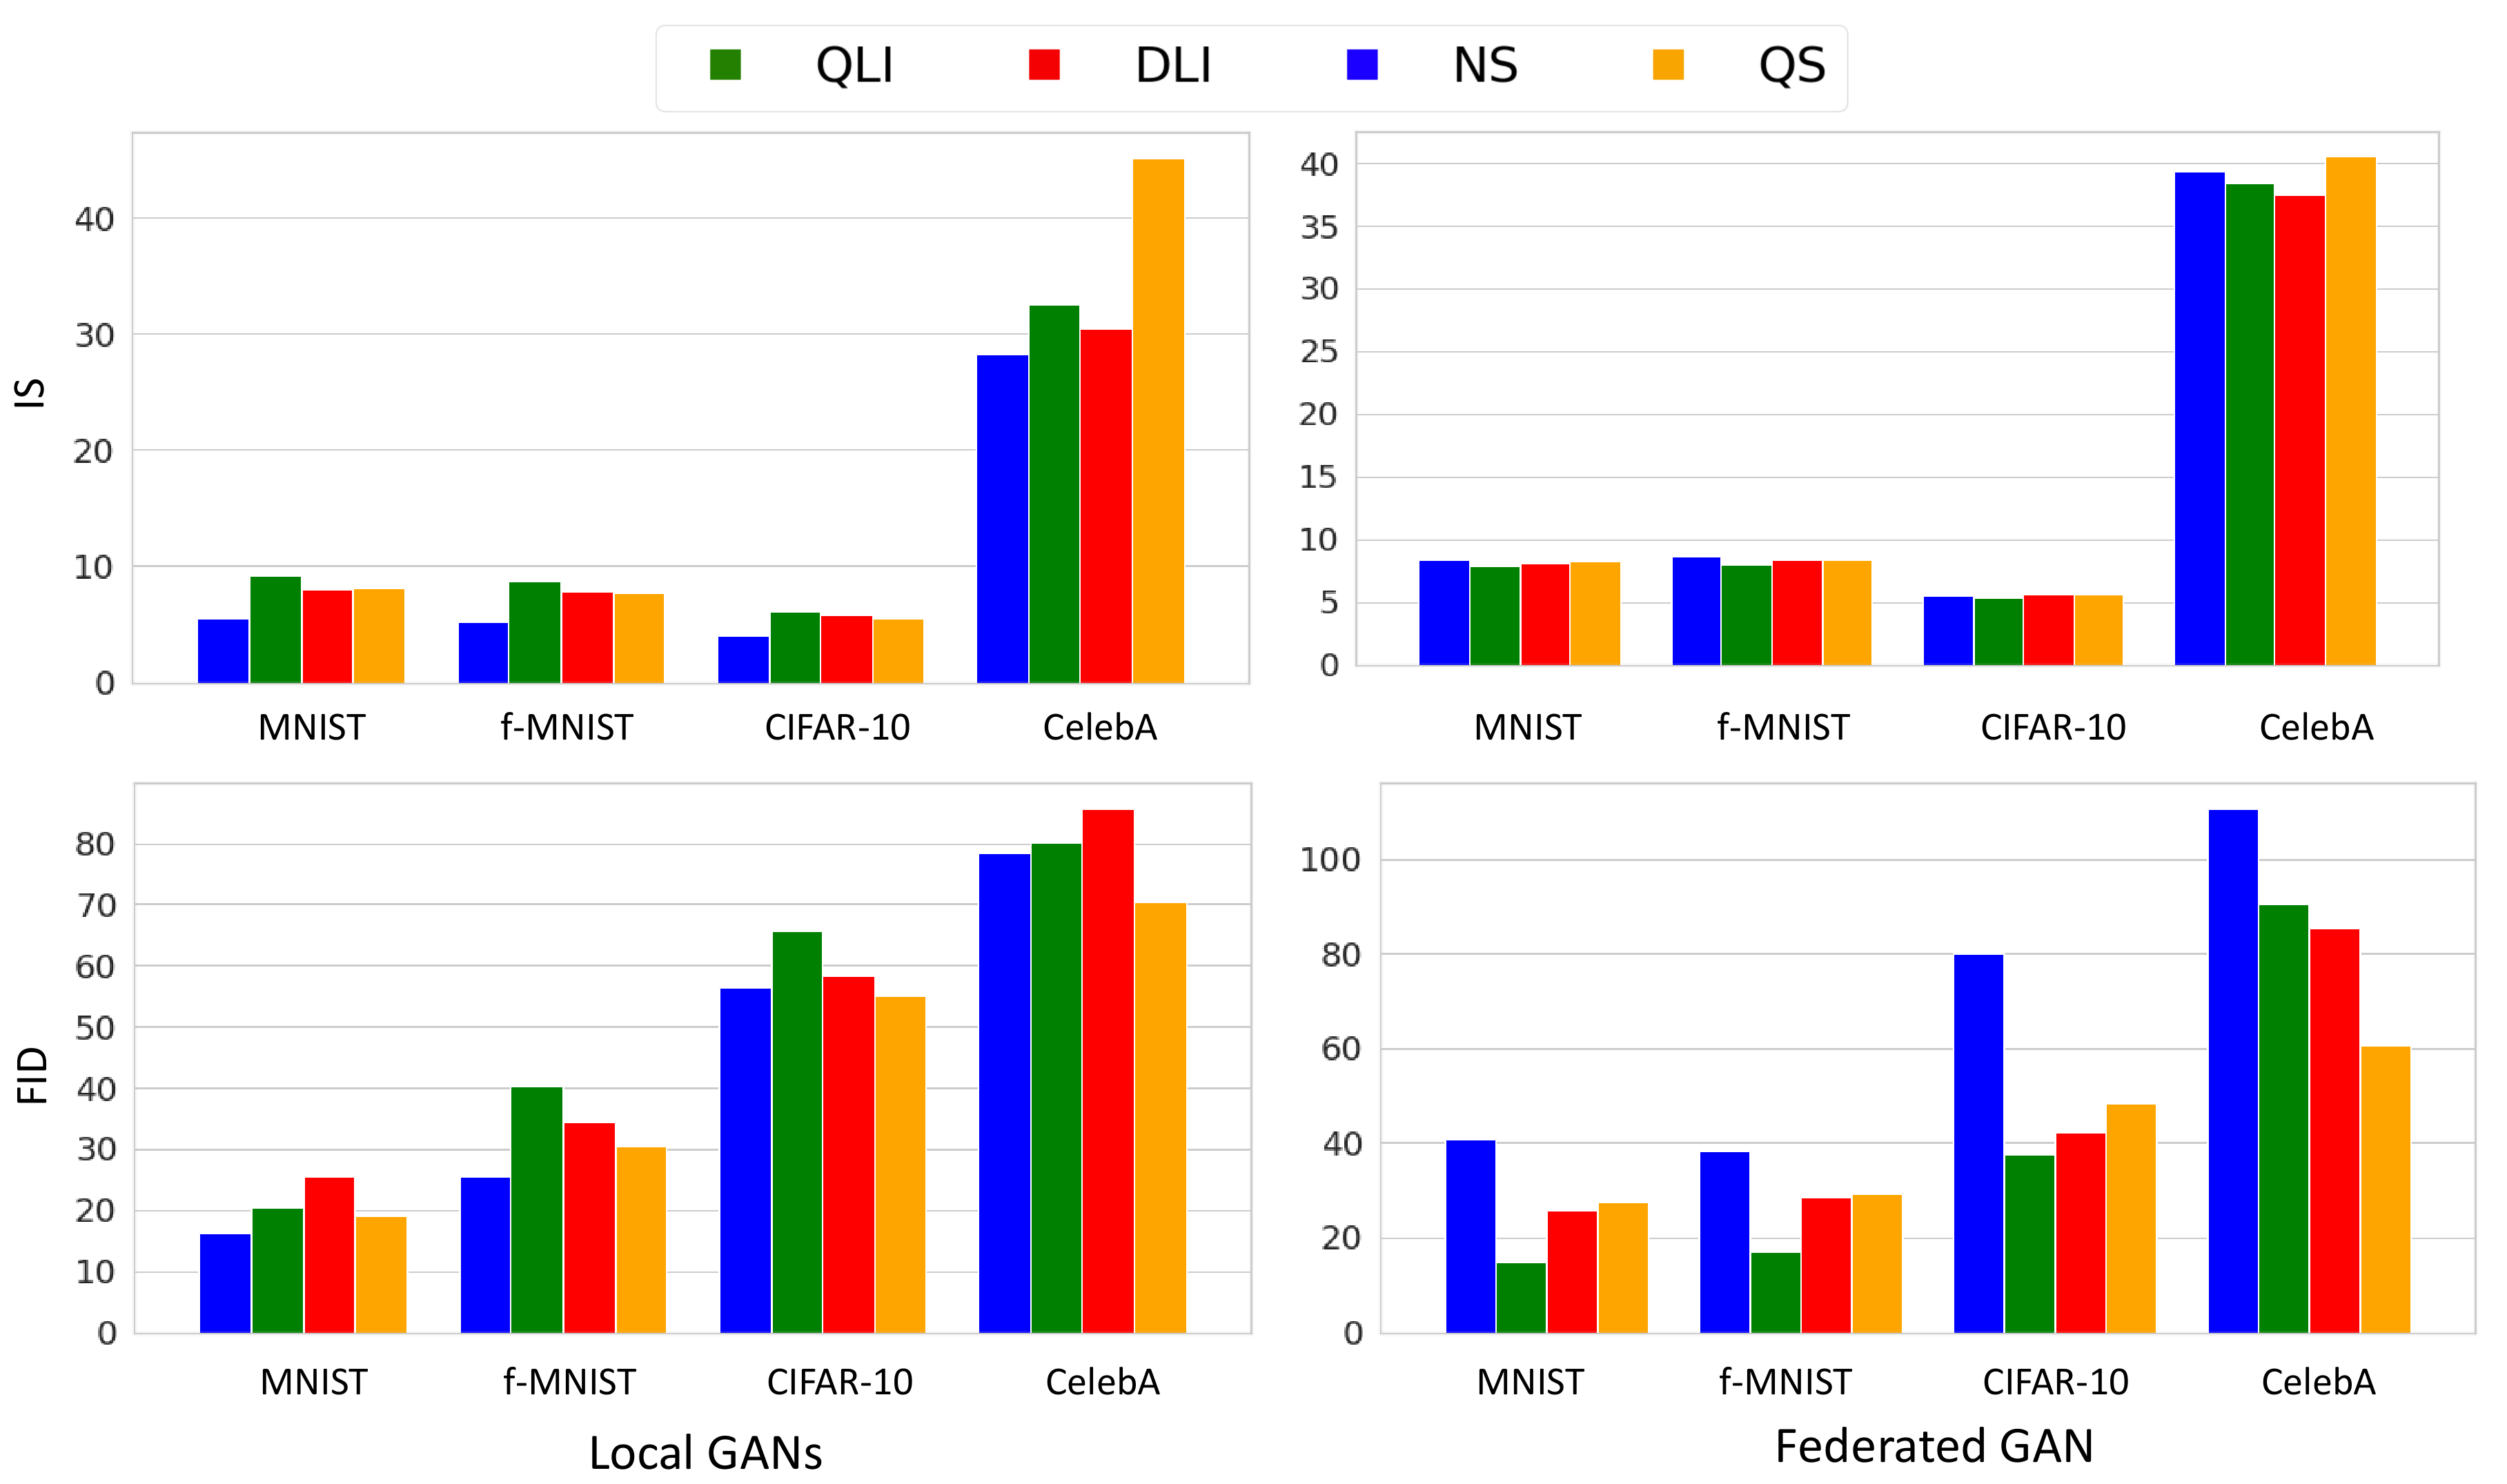
\includegraphics[width=0.7\linewidth]{Plots/baseline_IS_FID.png}
 \caption{Inception Score with Non-Private Local GANs and Federated GAN: The Figure shows the inception score and FID score for different distributions for each dataset in local GANs and federated  GAN with $K=10$. }
 \label{fig:baseline_IS}
\end{figure}








\begin{figure}
 \centering
 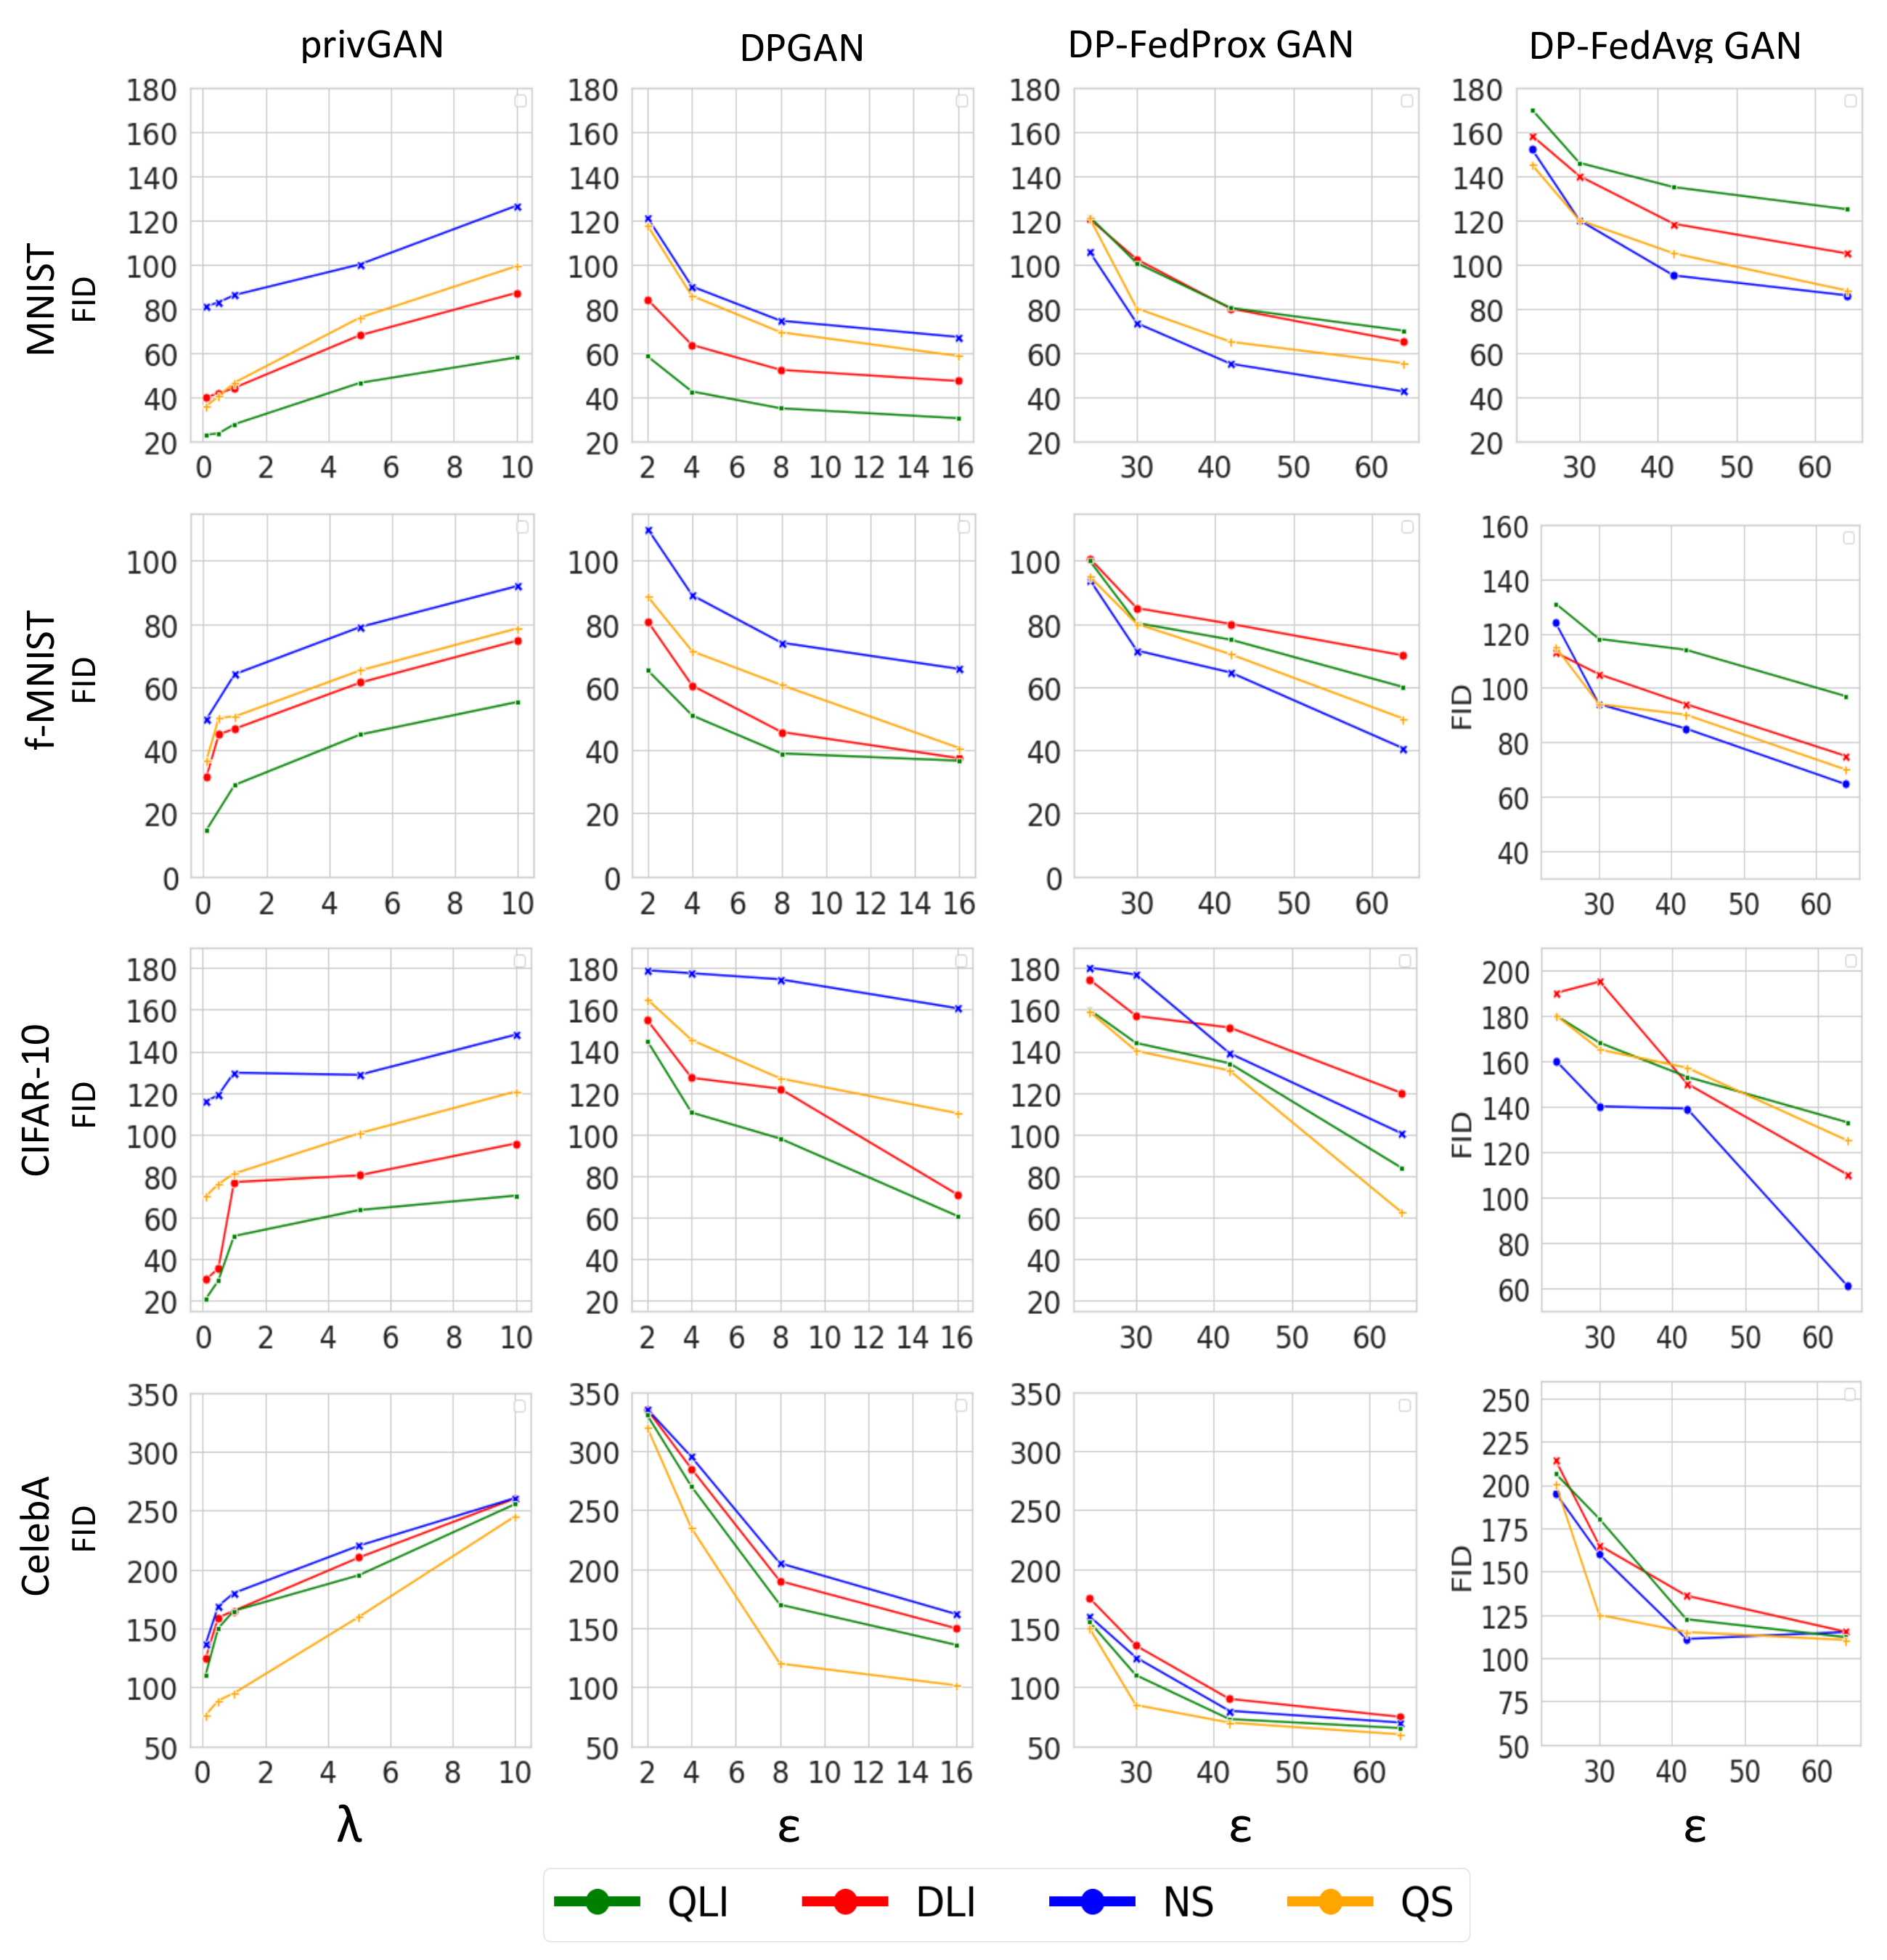
\includegraphics[width=0.8\linewidth]{Plots/vary_privacy_FID.png}
 \caption{Varying Privacy Parameters: The Figure illustrates FID Score for various privacy parameters in privGAN, DPGAN, DP-FedProx GAN, and DP-FedAvg GAN.}
 \label{fig:vary_privacy_FID}
\end{figure}


\begin{figure}
 \centering
 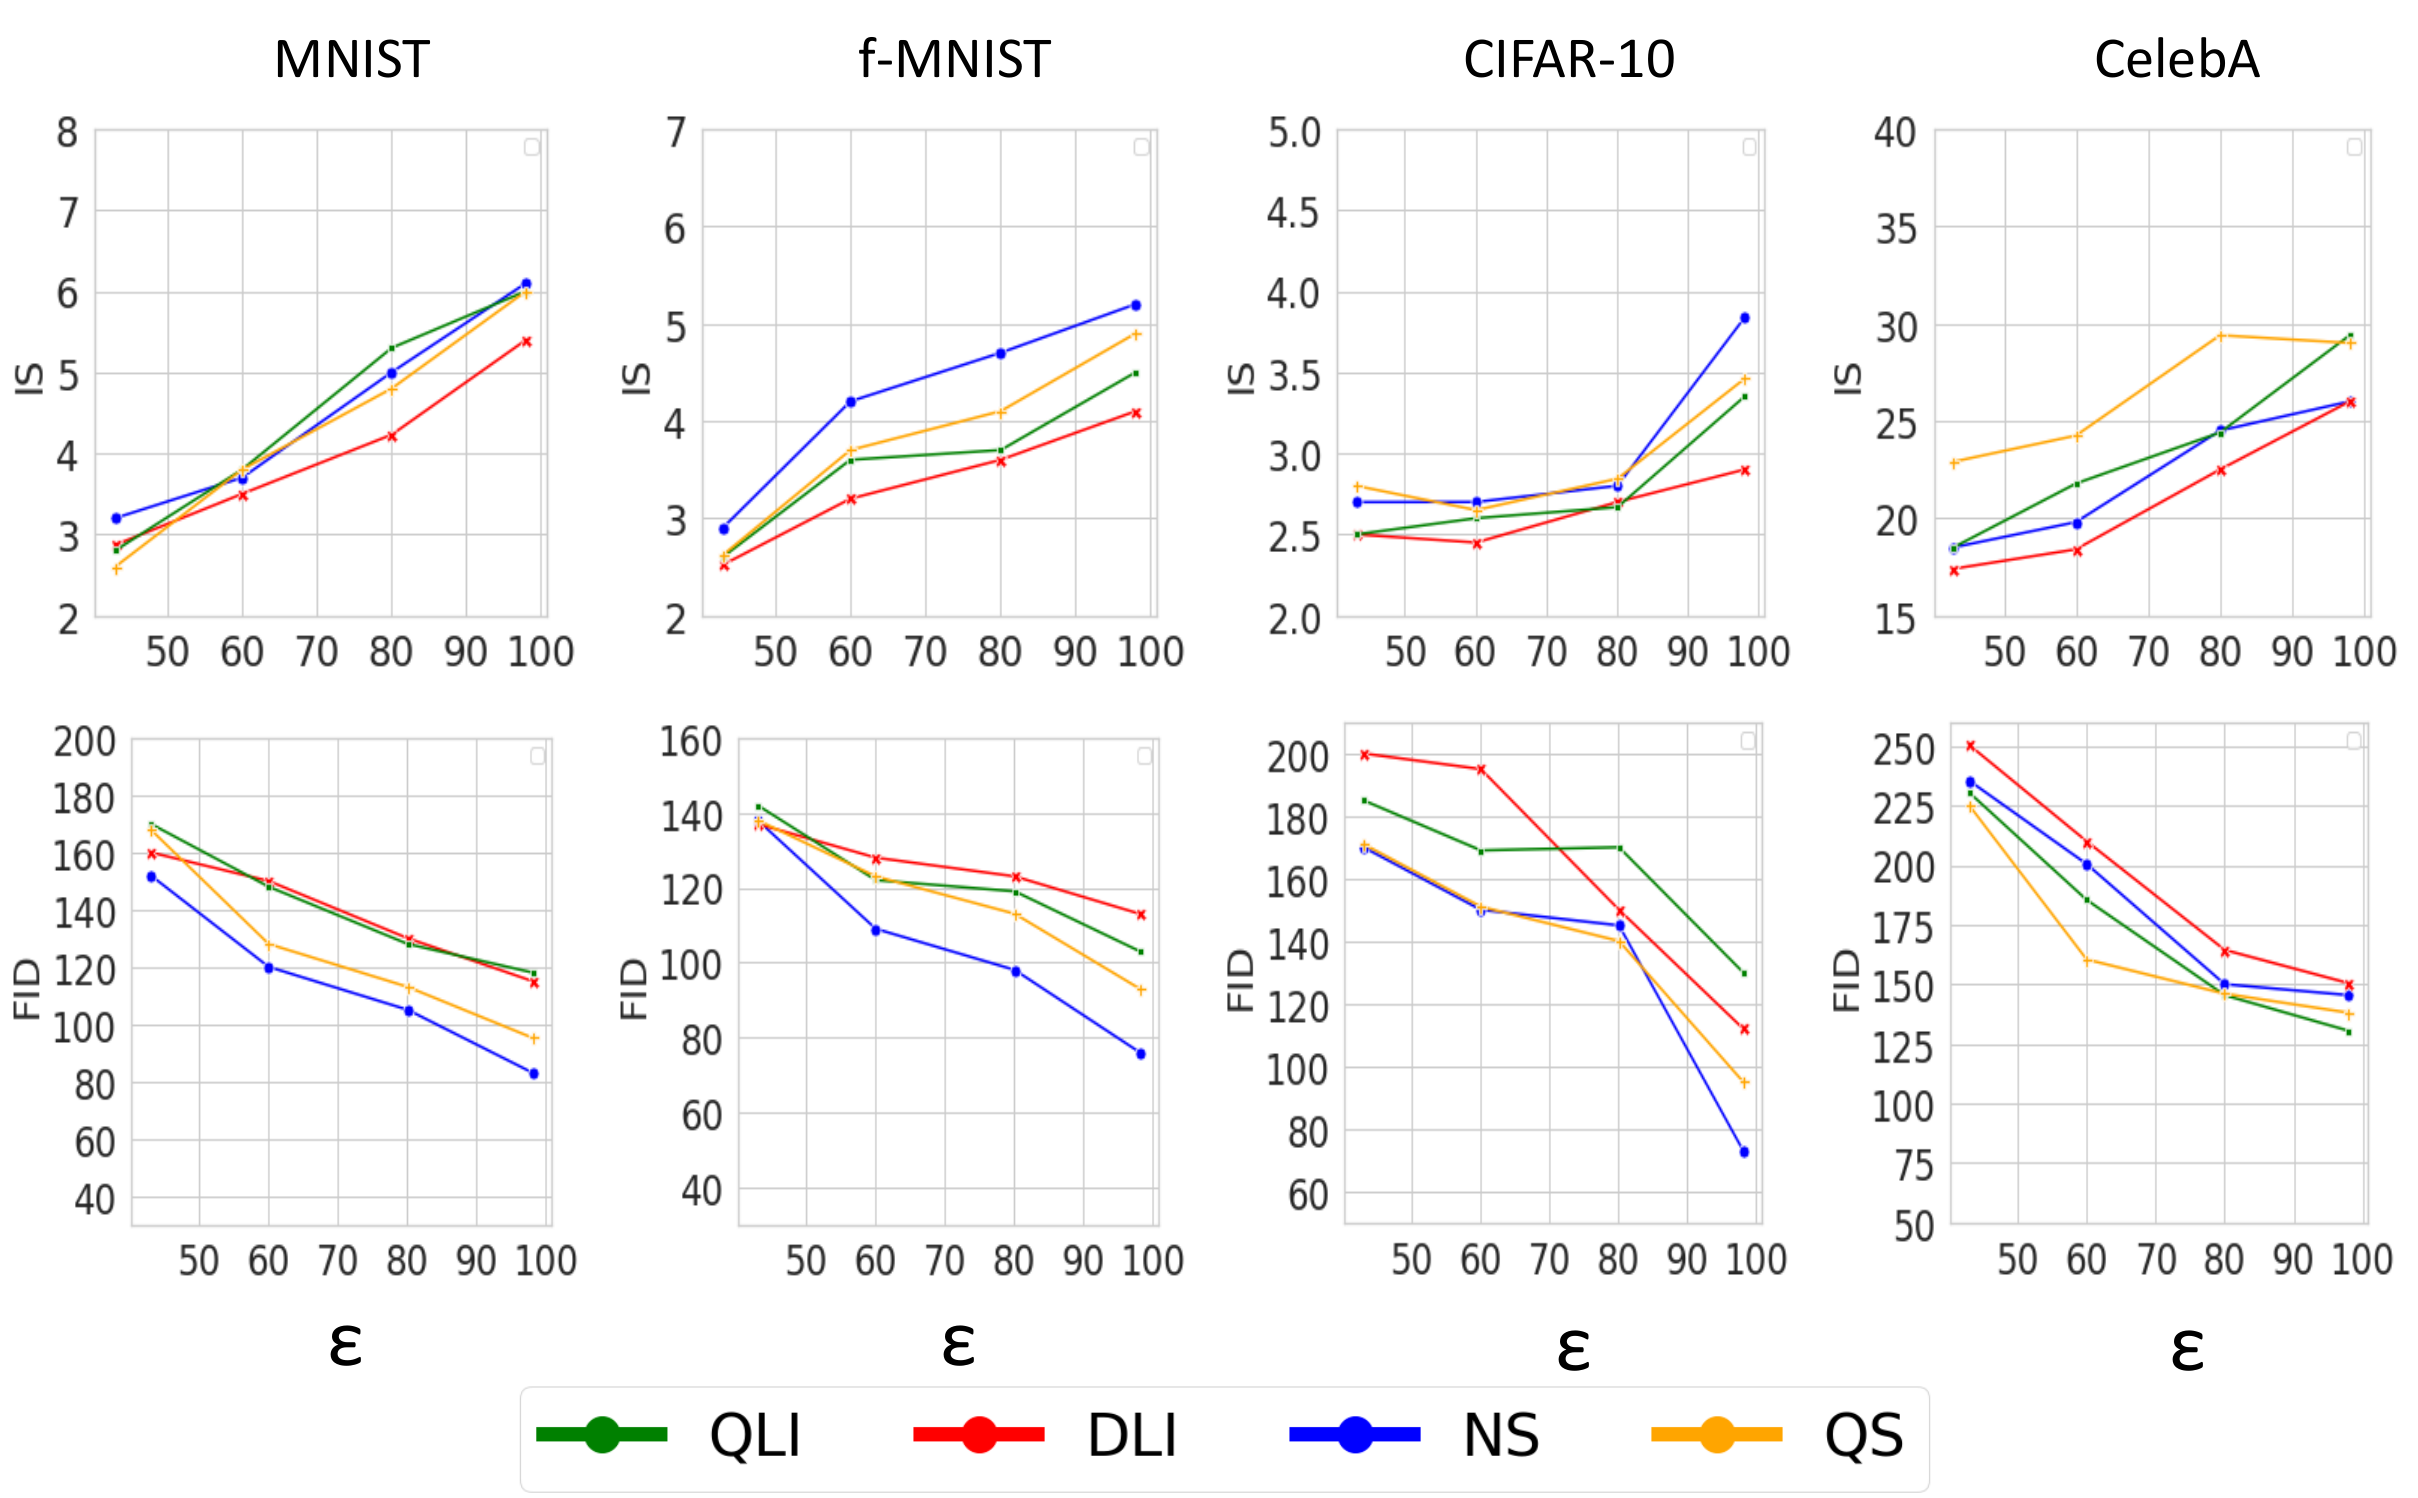
\includegraphics[width=0.8\linewidth]{Plots/vary_privacy_fedsgd.png}
 \caption{Varying Privacy Parameters in DP-FedSGD GAN: The Figure represents inception  and FID Score at various privacy parameters in DP-FedSGD GAN. DP-FedSGD GAN has the worst utility in terms of IS and FID compared to the DP-FedProx GAN and DP-FedAvg GAN, as shown in the Fig~\ref{fig:varyNoise} and ~\ref{fig:vary_privacy_FID}.} 
 \label{fig:vary_privacy_fedsgd}
\end{figure}


\begin{figure}
 \centering
 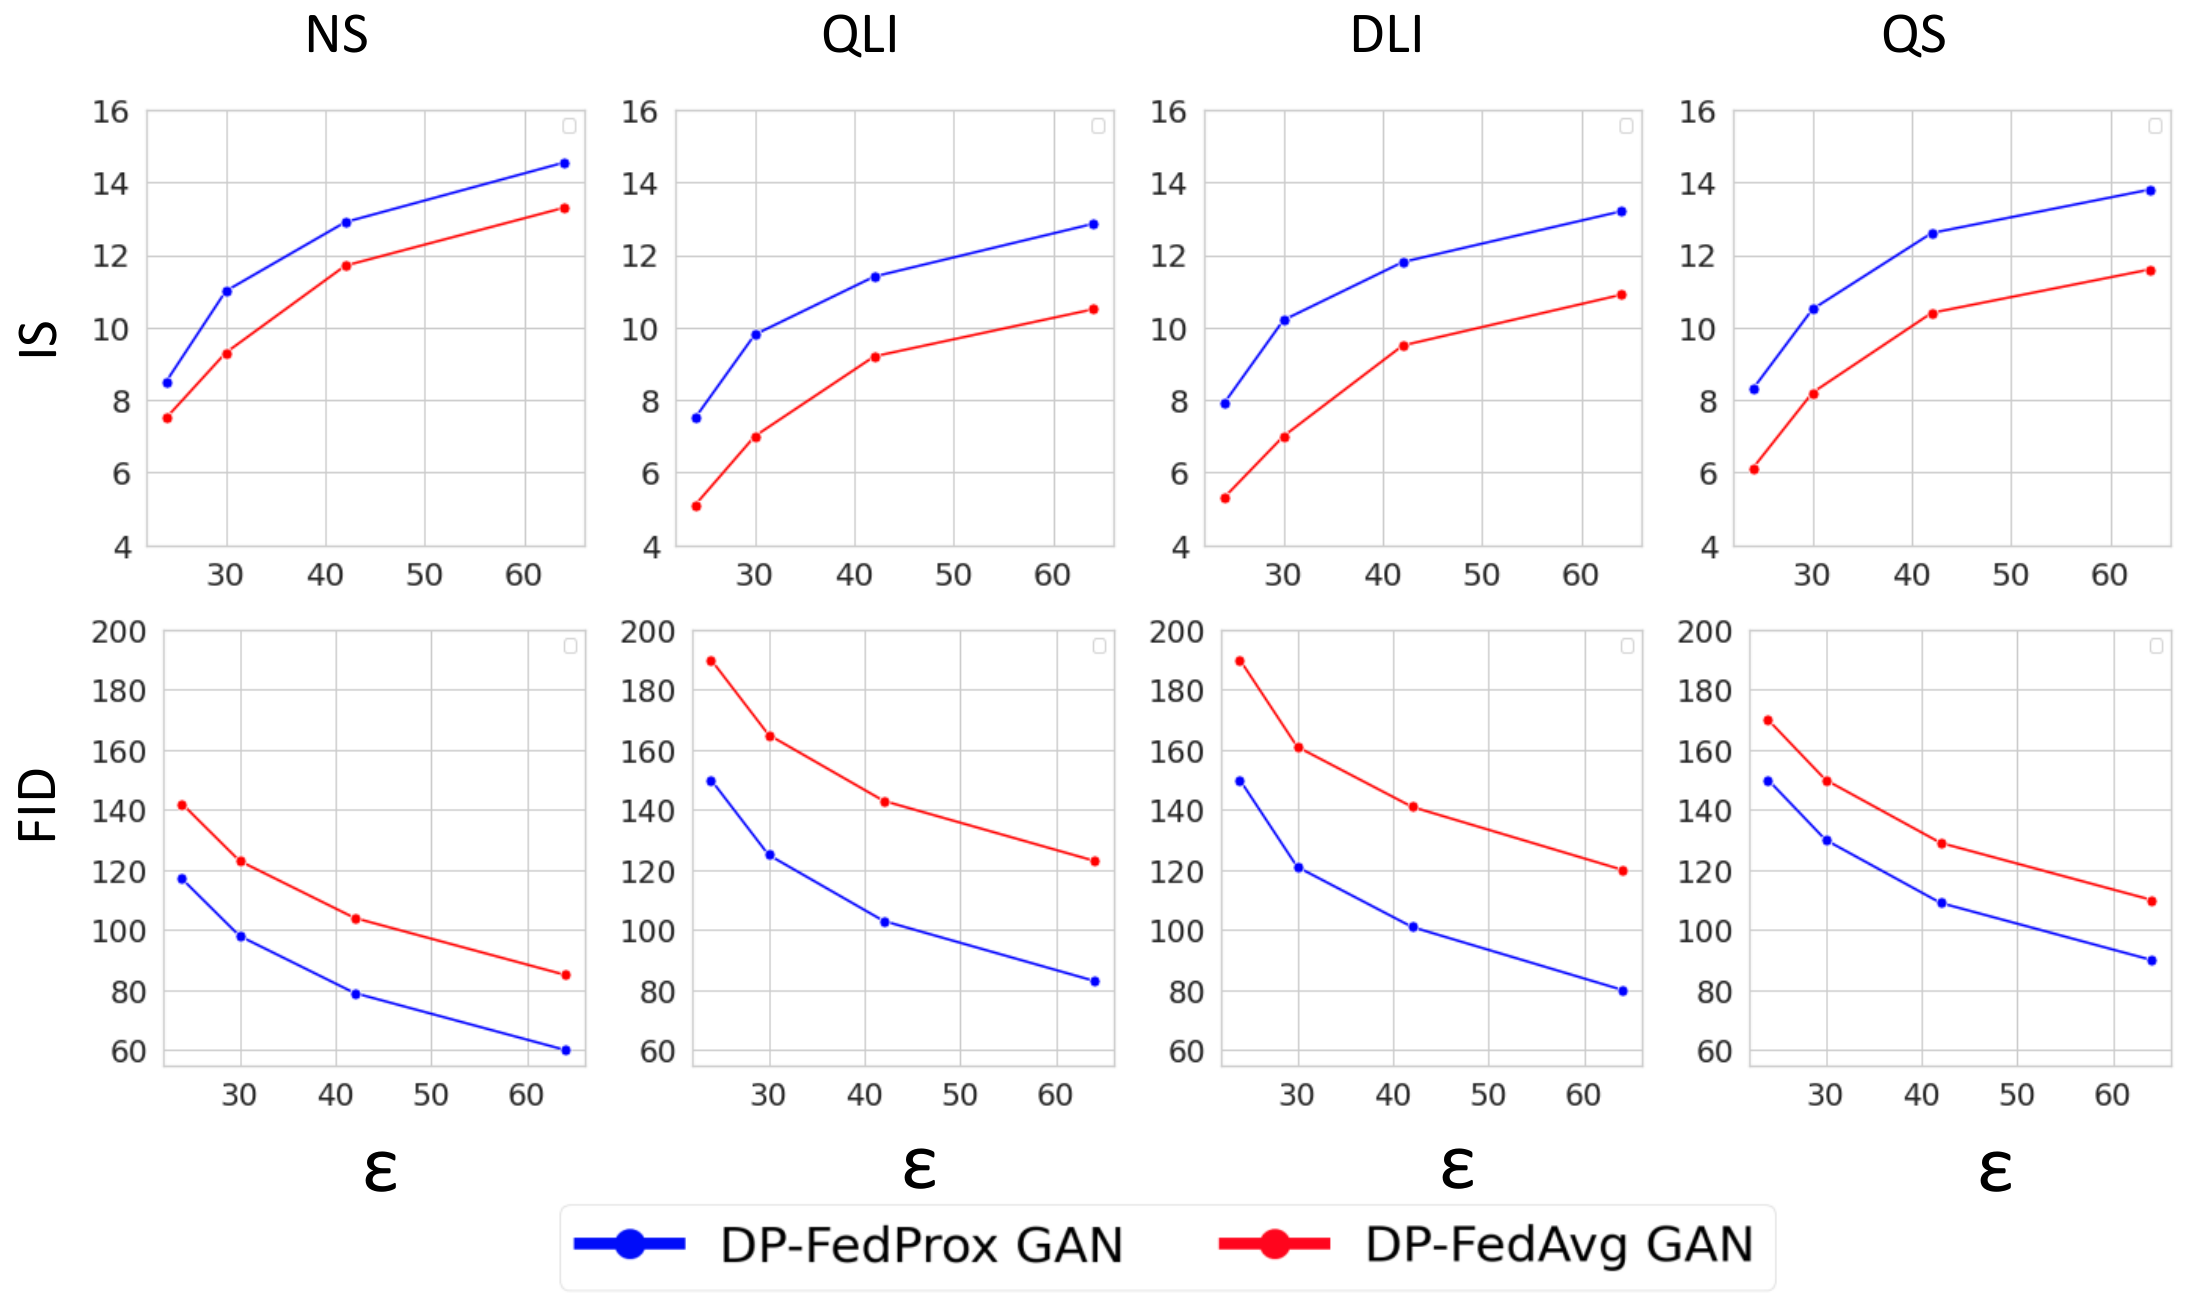
\includegraphics[width=0.7\linewidth]{Plots/varyNoise_emnist.png}
	\caption{\small Varying Privacy Parameters on EMNIST. The Figure depicts the inception and FID score  at various privacy parameters in DP-FedProx GAN and DP-FedAvg GAN at K=500 on EMNIST. }
 \label{fig:varyNoise_emnist}
\end{figure}

\begin{figure}
 \centering
 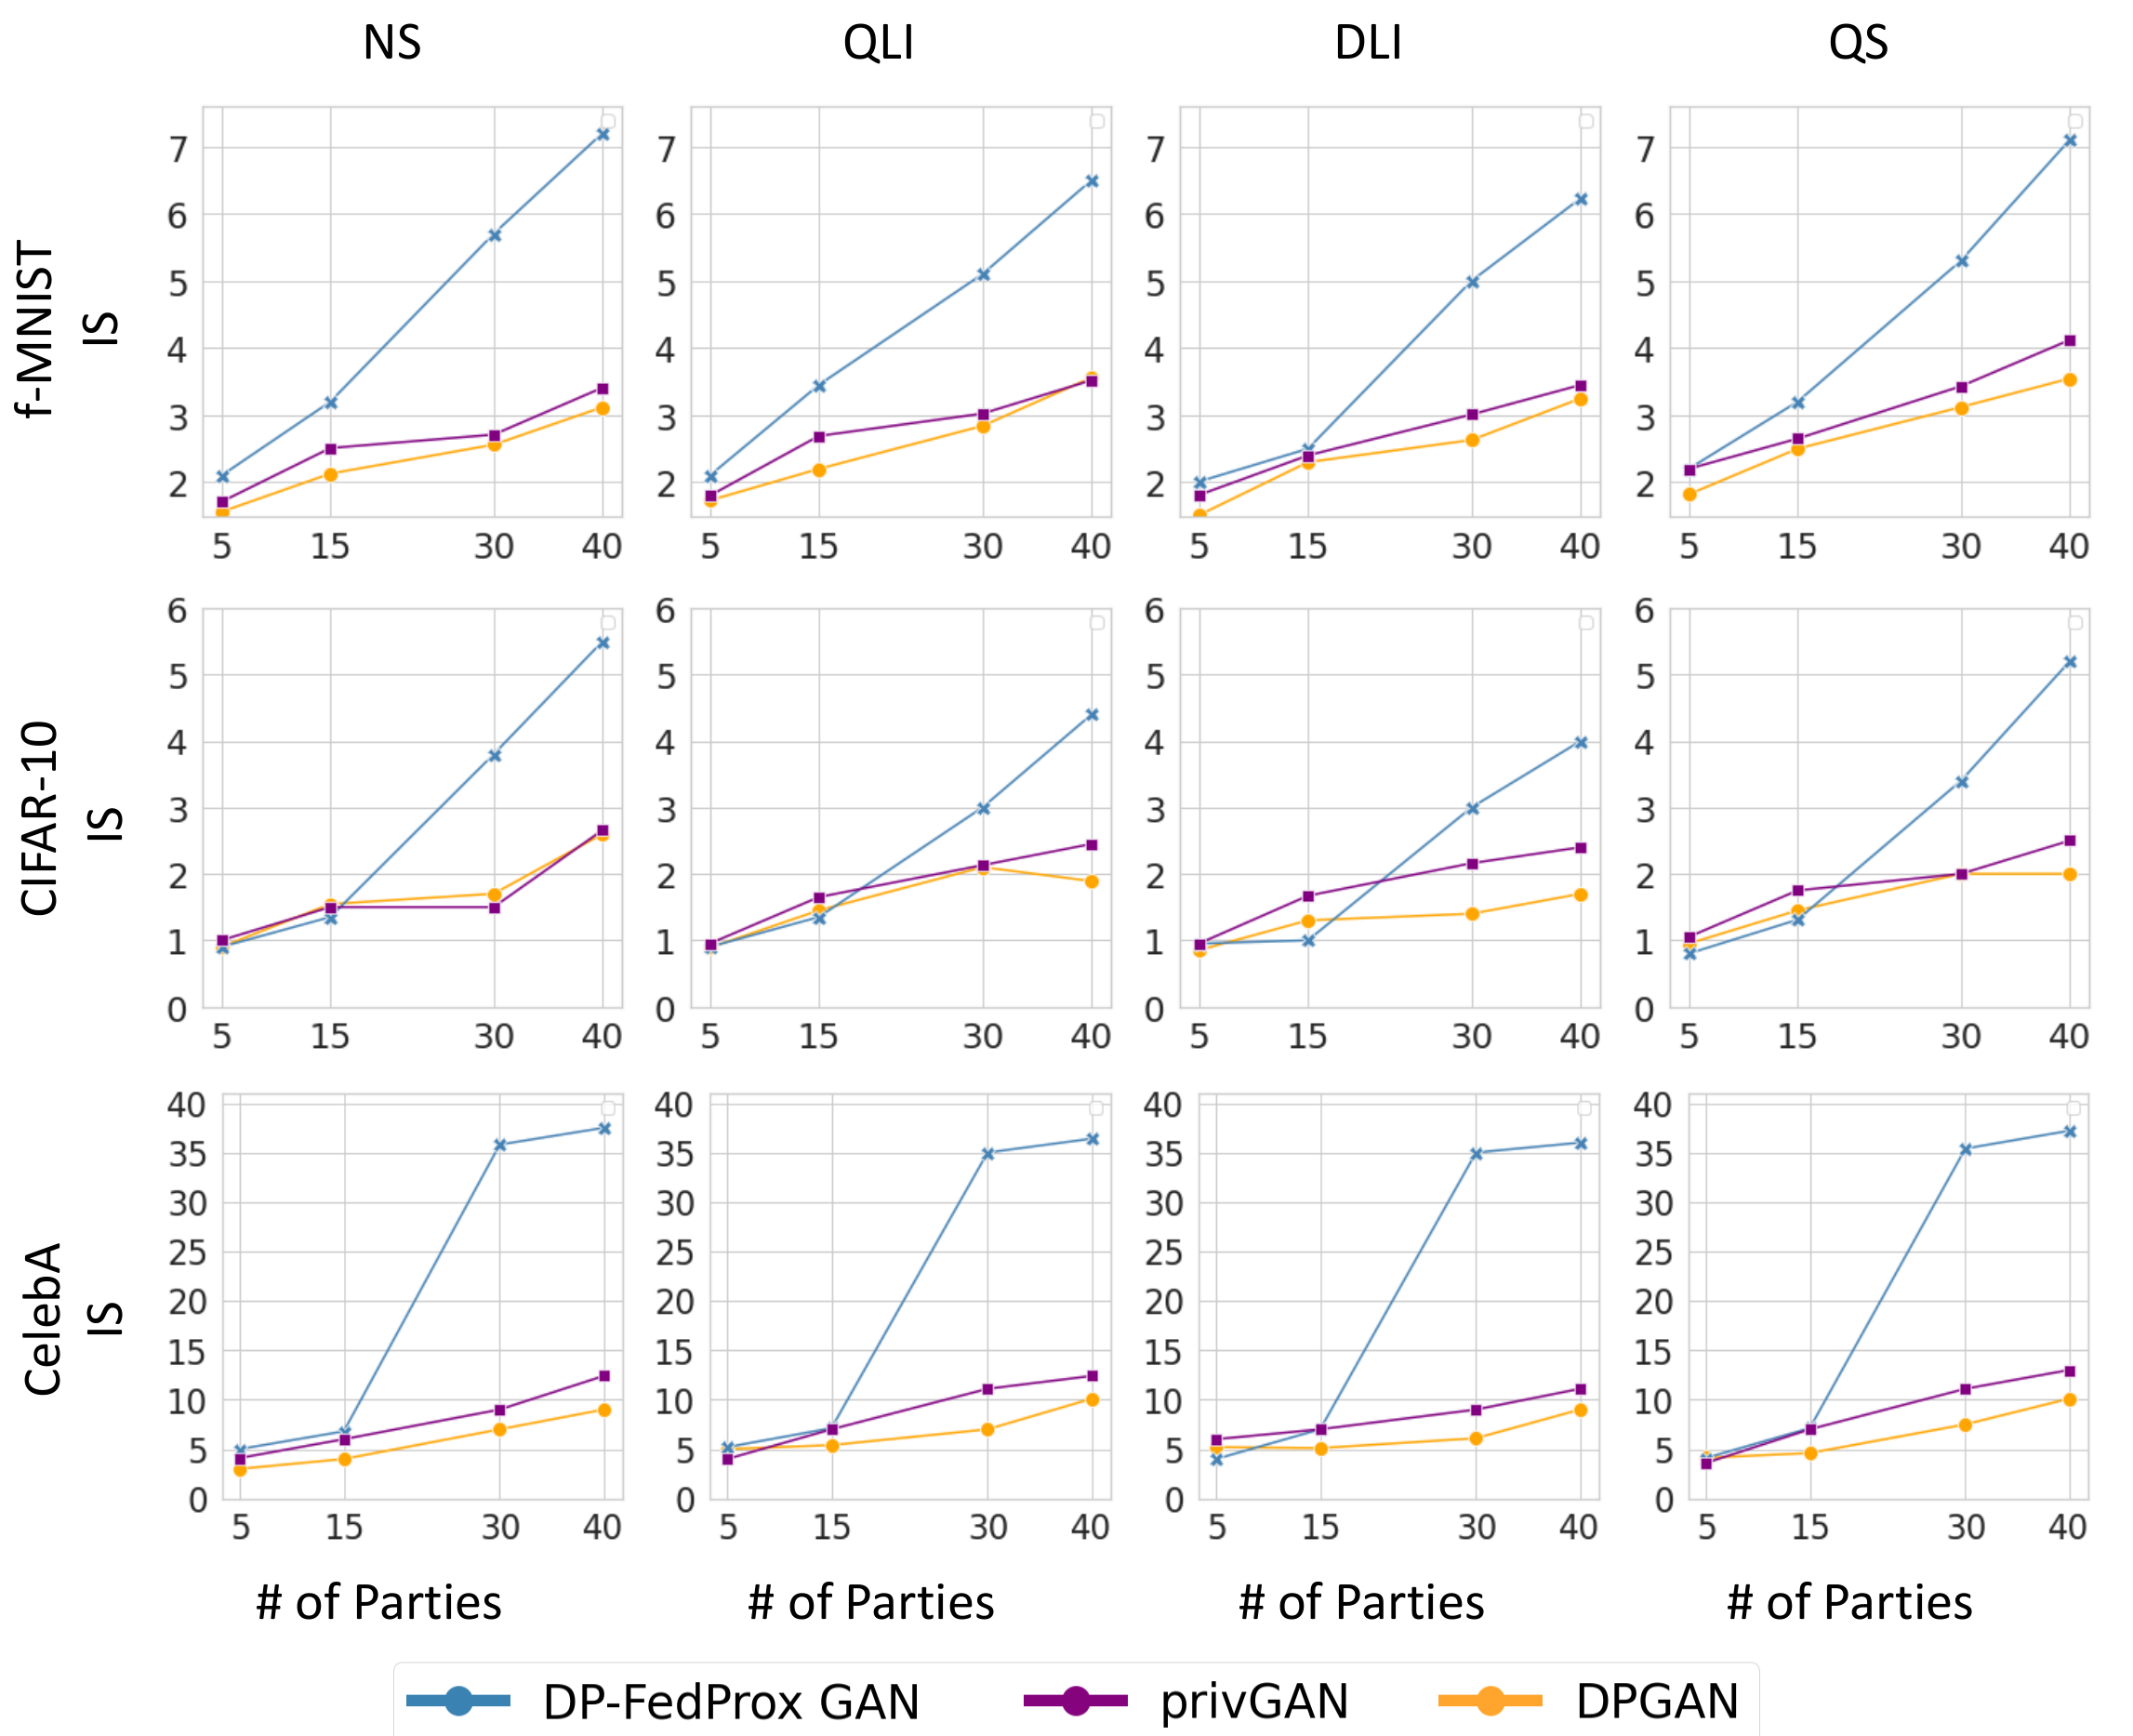
\includegraphics[width=0.8\linewidth]{Plots/vary_parties_IS.png}
 \caption{Varying Number of Parties: The Figure depicts the inception score for various distributions at various numbers of parties in privGAN, DPGAN, and DP-FedProx GAN.}

 
 \label{fig:vary_parties_IS}
\end{figure}



% \begin{figure}
%  \centering
%  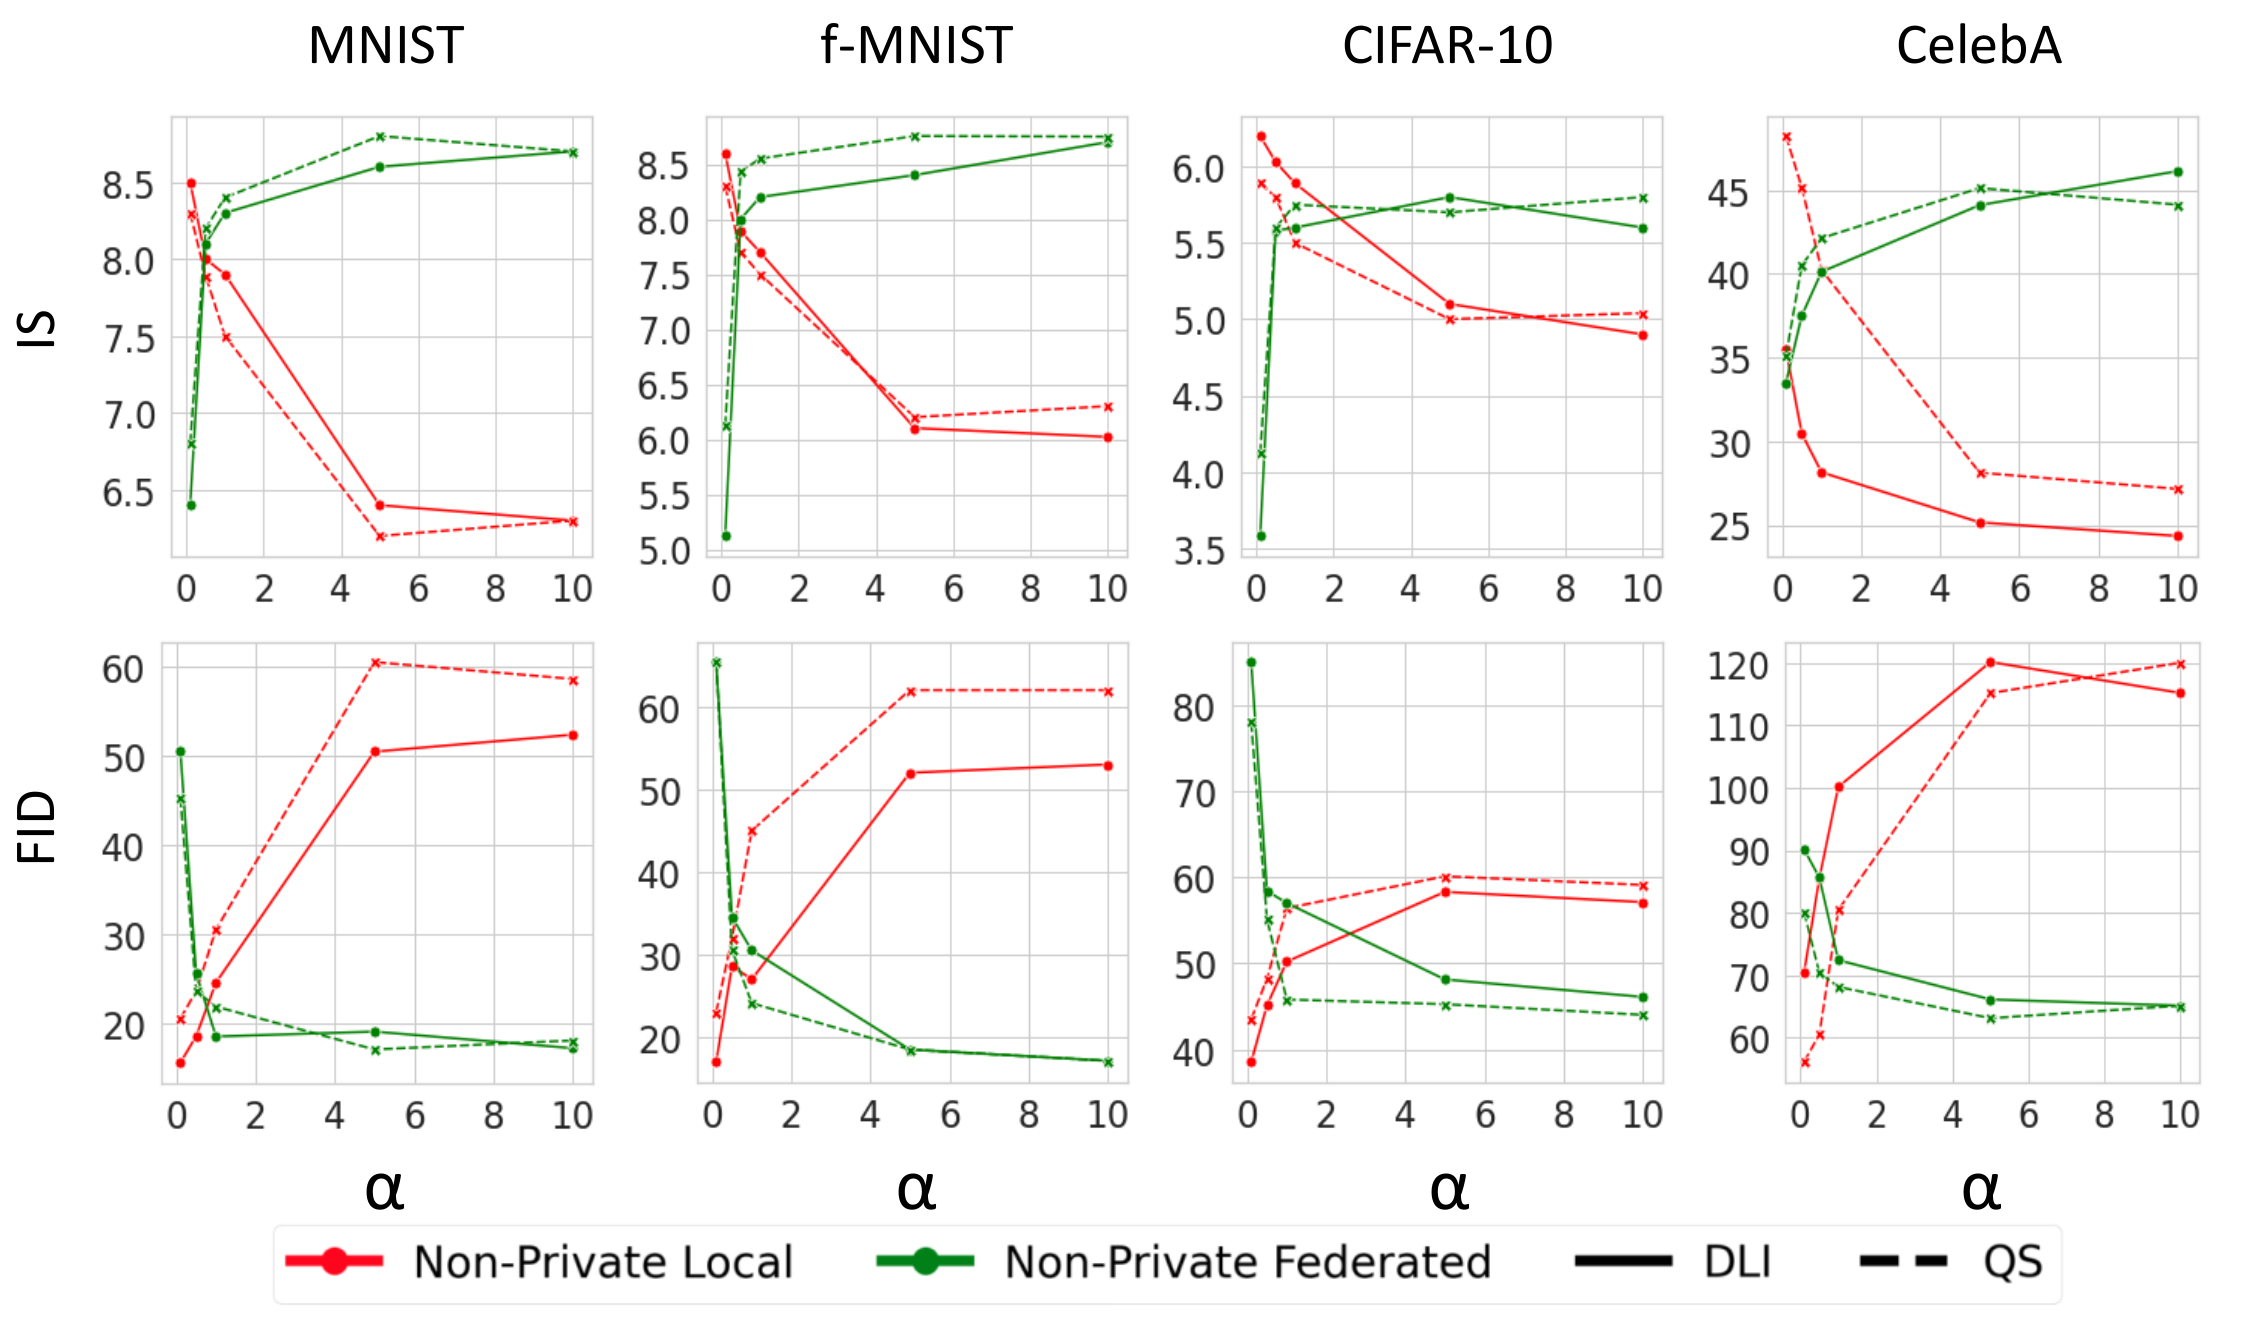
\includegraphics[width=0.8\linewidth]{Plots/nonprivate_vary_alpha_utility.png}
%  \caption{Varying Concentration Parameter for Non-Private Local GANs and Federated GAN: The Figure shows the inception and FID score for different distributions at various concentration parameters in local GANs and federated  GAN with $K=10$. }
%  \label{fig:nonprivate_vary_alpha_utility}
% \end{figure}

\begin{figure}
 \centering
 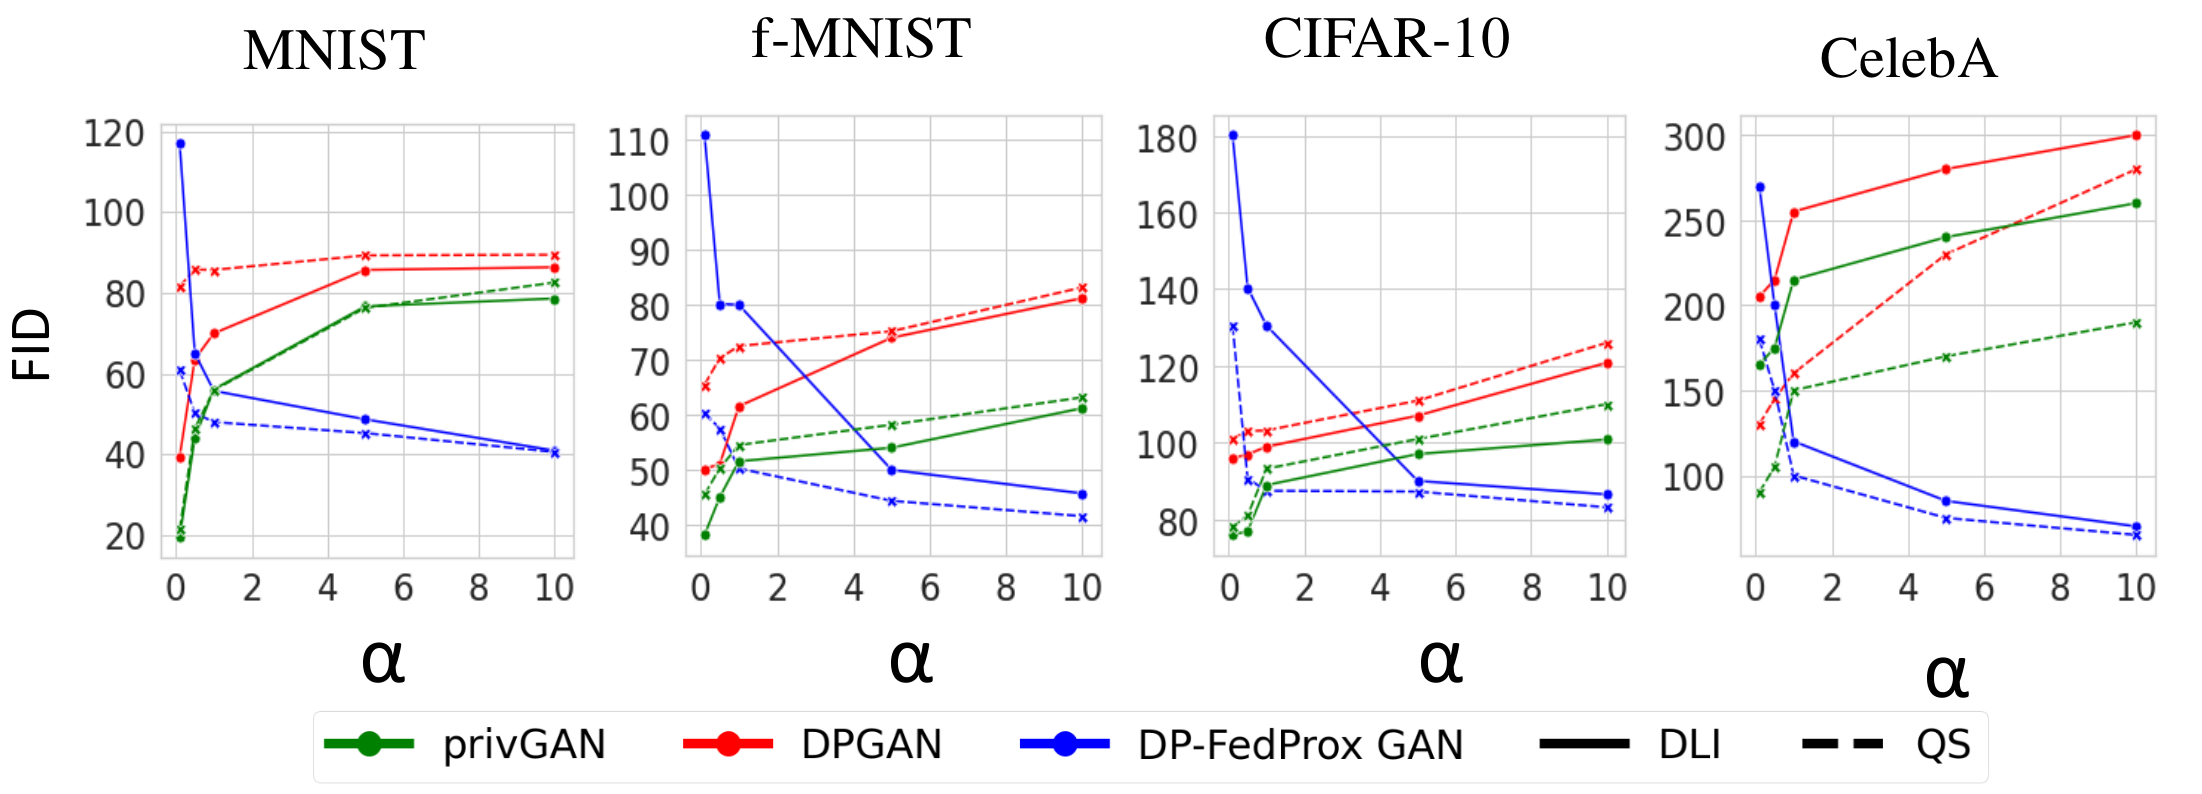
\includegraphics[width=0.8\linewidth]{Plots/vary_alpha_FID.png}
 \caption{Varying Concentration Parameters: The Figure illustrates the FID score for different distributions at various concentration parameters in privGAN, DPGAN, and DP-FedProx GAN. }
 \label{fig:vary_alpha_FID}
\end{figure}




% \begin{figure}
%  \centering
%  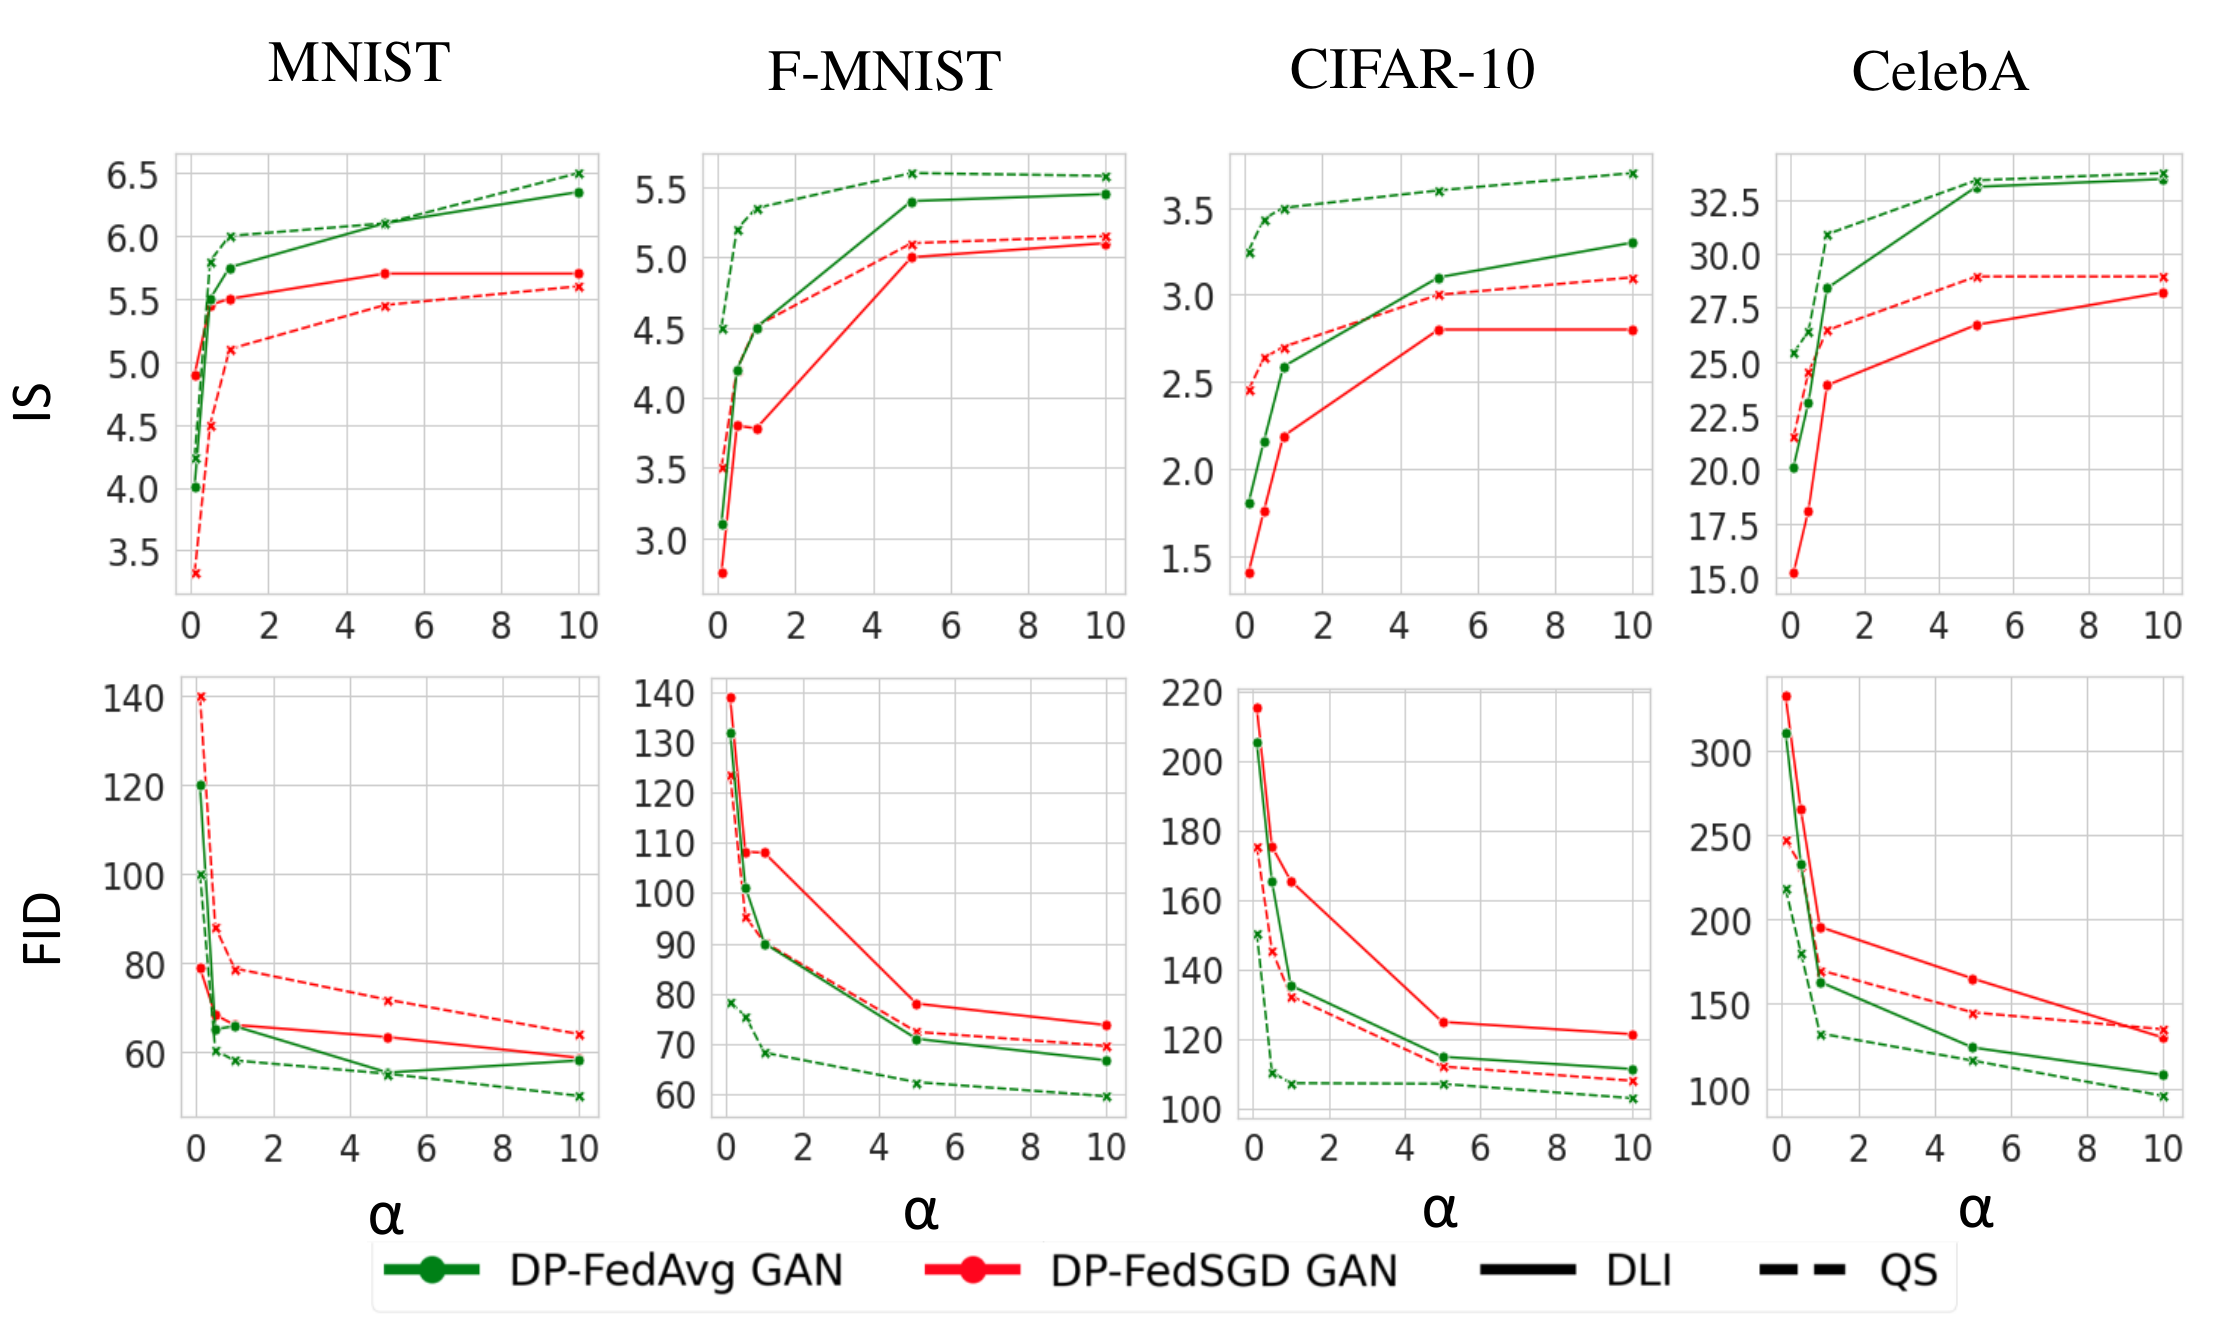
\includegraphics[width=0.8\linewidth]{Plots/vary_alpha_fedsgd_fedavg.png}
%  \caption{Varying Concentration Parameters in DP-FedAvg GAN and DP-FedSGD GAN: The Figure displays the inception and FID score for various distributions at various concentration parameters in the DP-FedAvg GAN and the DP-FedSGD GAN models.}
%  \label{fig:vary_alpha_fedsgd_fedavg}
% \end{figure}




\begin{figure}
 \centering
 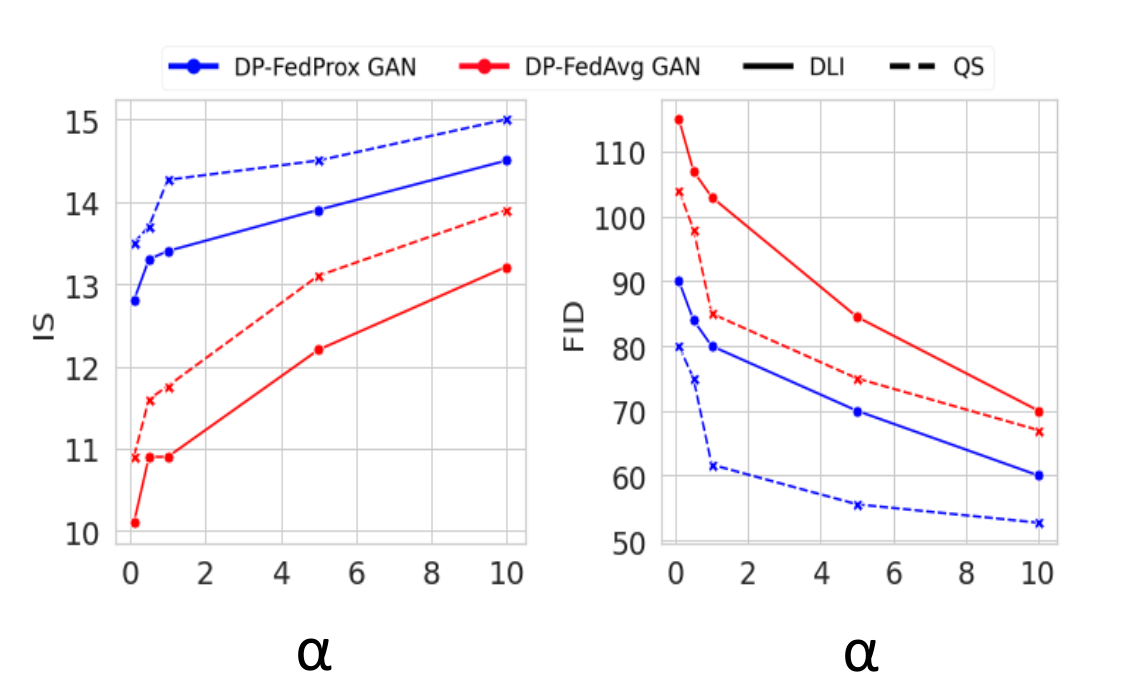
\includegraphics[width=0.45\linewidth]{Plots/varyAlpha_emnist.png}
	\caption{\small Varying Concentration Parameter on EMNIST with 500 Parties ($K$=500) using DP-FedProx GAN  and DP-FedAvg GAN .}
 \label{fig:varyAlpha_emnist}
\end{figure}


% \begin{figure}
%  \centering
%  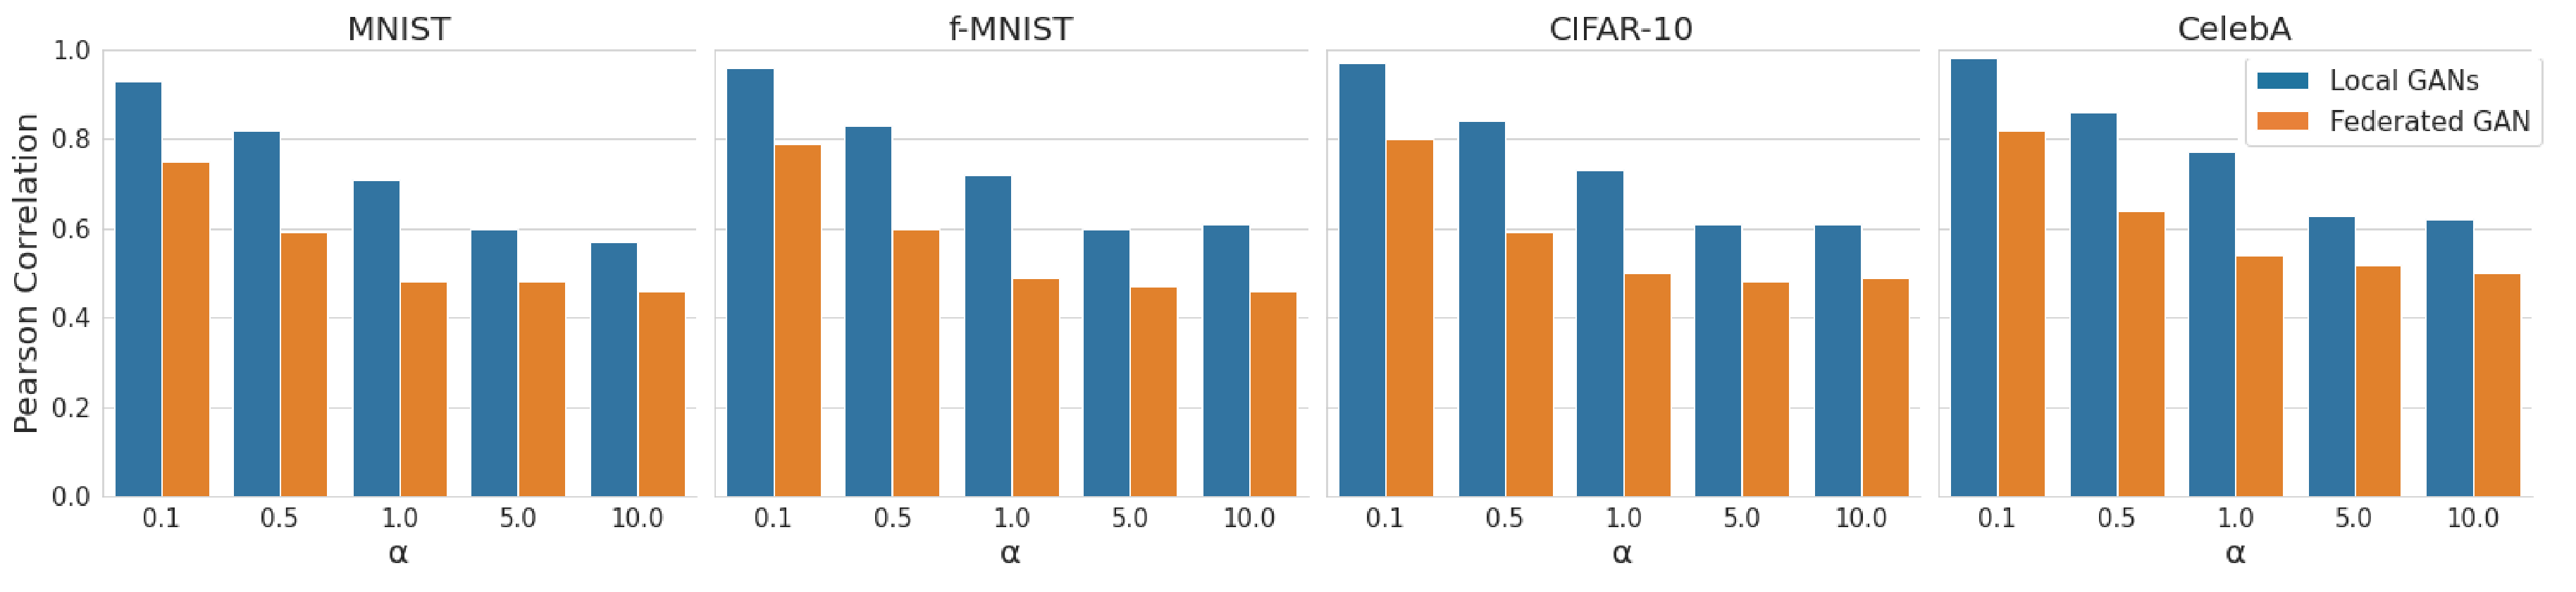
\includegraphics[width=0.8\linewidth]{Plots/IS_alpha_nonprivate.png}
%  \caption{Vary Concentration Parameters in QS distribution: The Figure depicts Pearson correlation $r$ between local data size and local IS at various concentration parameters $\alpha$ in Local GANs and Federated GAN at $K=10$. The correlation in Federated GAN cannot be evaluated directly due to synthetic samples provided by the central server. For the Federated GAN, we evaluated each local party's impact on overall IS by calculating the difference in IS when all parties' data was utilized versus excluding the data from a specific local party.  }
%  \label{fig:IS_alpha_nonprivate}
% \end{figure}



% \begin{figure}
%  \centering
%  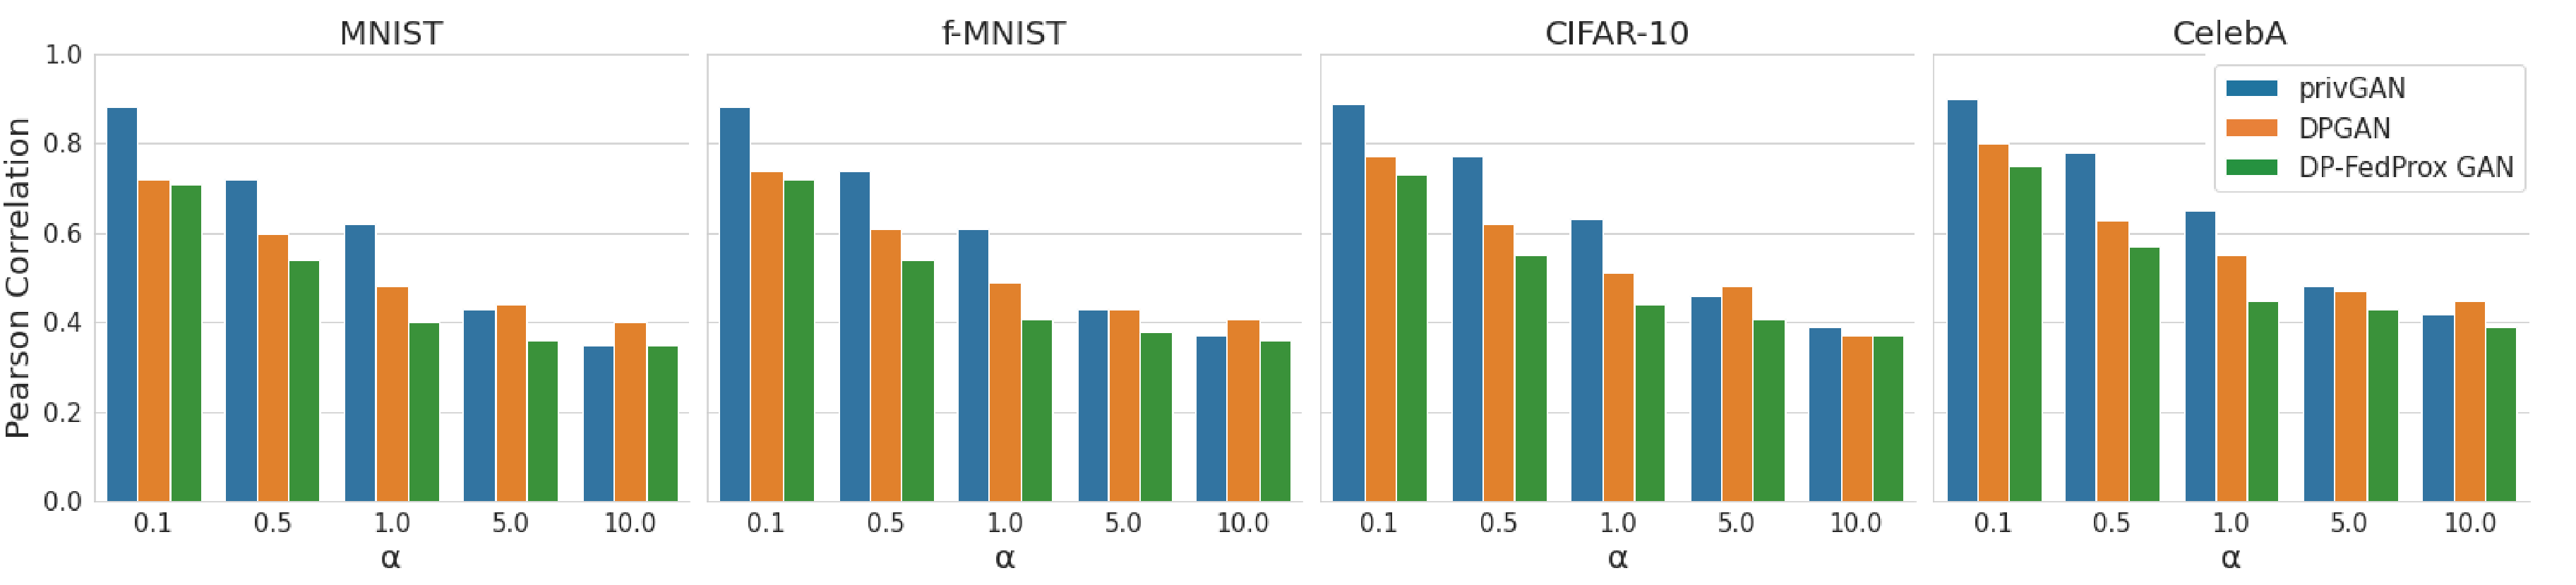
\includegraphics[width=0.8\linewidth]{Plots/IS_alpha_private.png}
%  \caption{Vary Concentration Parameters in QS distribution: The Figure depicts Pearson correlation $r$ between local data size and local IS at various concentration parameters $\alpha$ in privGAN, DPGAN,  and DP-FedProx GAN. For the DP-FedProx GAN, we evaluated each local party's impact on overall IS by calculating the difference in IS when all parties' data was utilized versus excluding the data from a specific local party.  }
%  \label{fig:IS_alpha_private}
% \end{figure}


% \begin{figure}
%  \centering
%  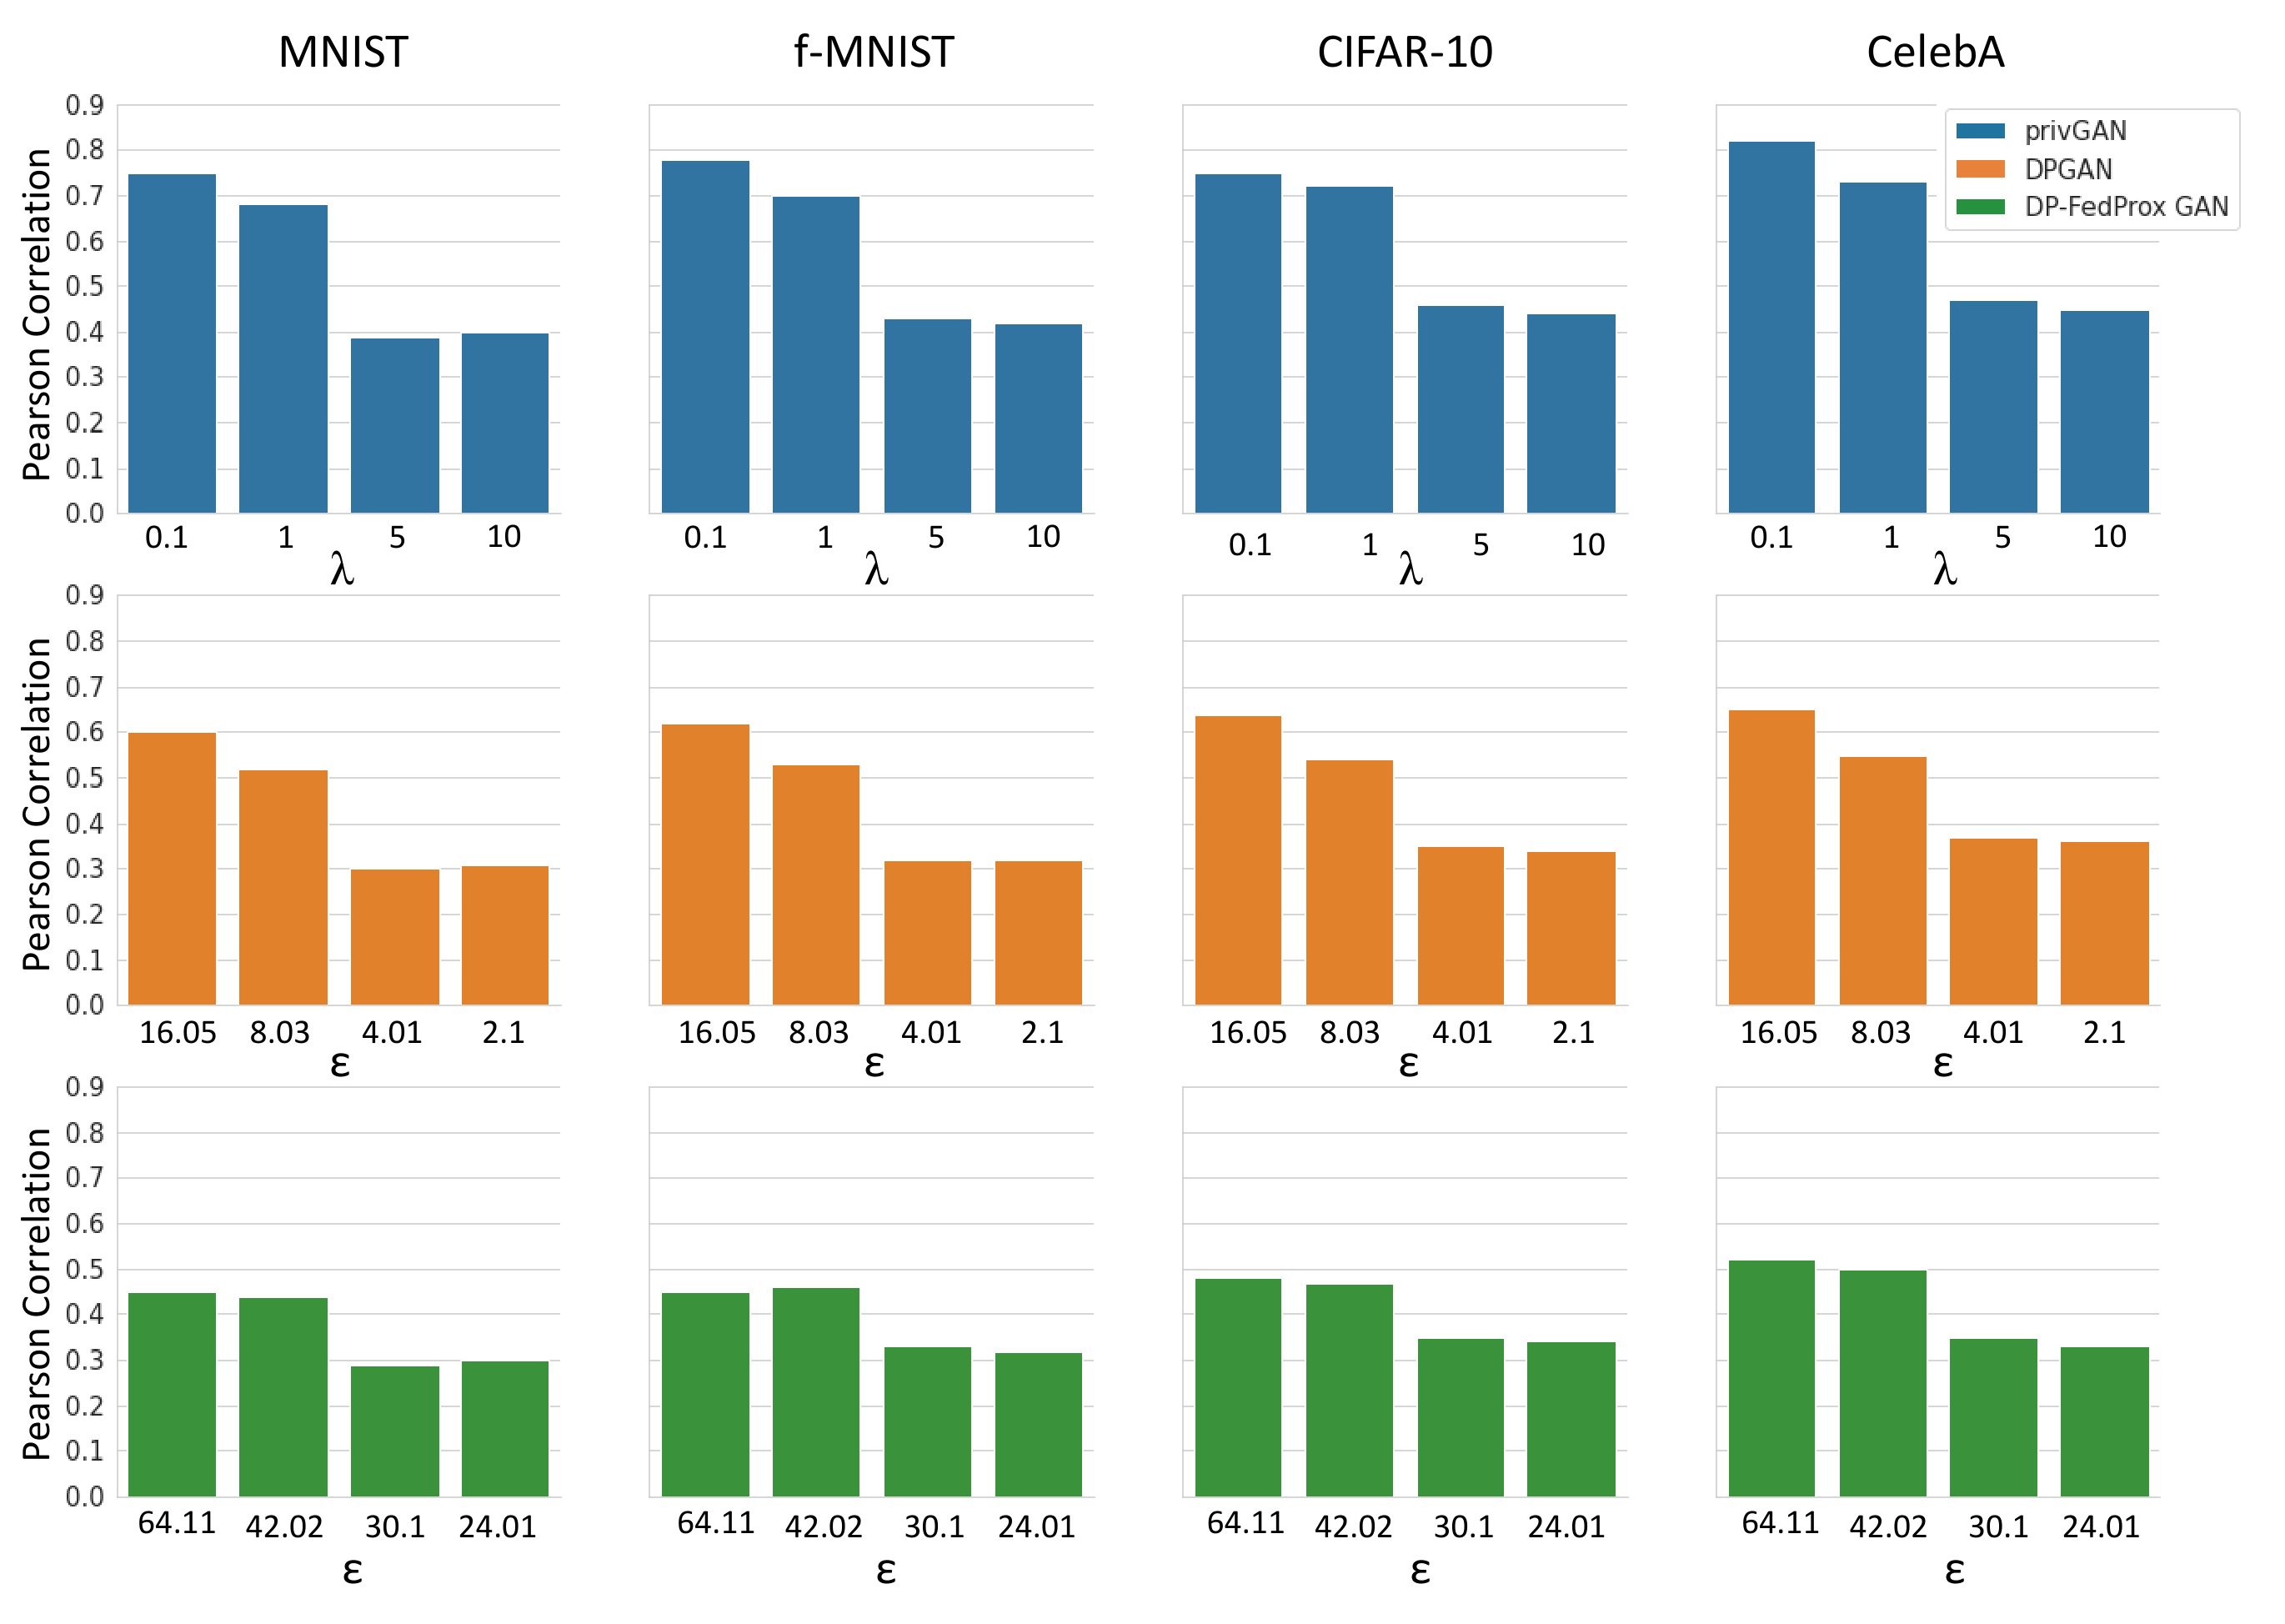
\includegraphics[width=0.8\linewidth]{Plots/IS_noise_private.png}
%  \caption{Vary Privacy Parameters in QS distribution: The Figure depicts Pearson correlation $r$ between local data size and local IS at various privacy parameters in privGAN, DPGAN, and DP-FedProx GAN. We assessed each local party's impact on overall IS for the DP-FedProx GAN by computing the difference in IS when all parties' data was used versus excluding data from a specific local party. }
%  \label{fig:IS_noise_private}
% \end{figure}





% \begin{figure}
%  \centering
%  \includegraphics[width=0.6\linewidth]{Plots/IS_local_gans_varyalpha_corr.png}
%  \caption{Vary Concentration Parameters in QS distribution: The Figure depicts Pearson correlation $r$ between local data size and local IS at various concentration parameters $\alpha$ in privGAN and DPGAN. The correlation in DP-FedProx GAN cannot be evaluated directly due to synthetic samples provided by the central server.  }
%  \label{fig:IS_local_gans_varyalpha_corr}
% \end{figure}



% \begin{figure}
%  \centering
%  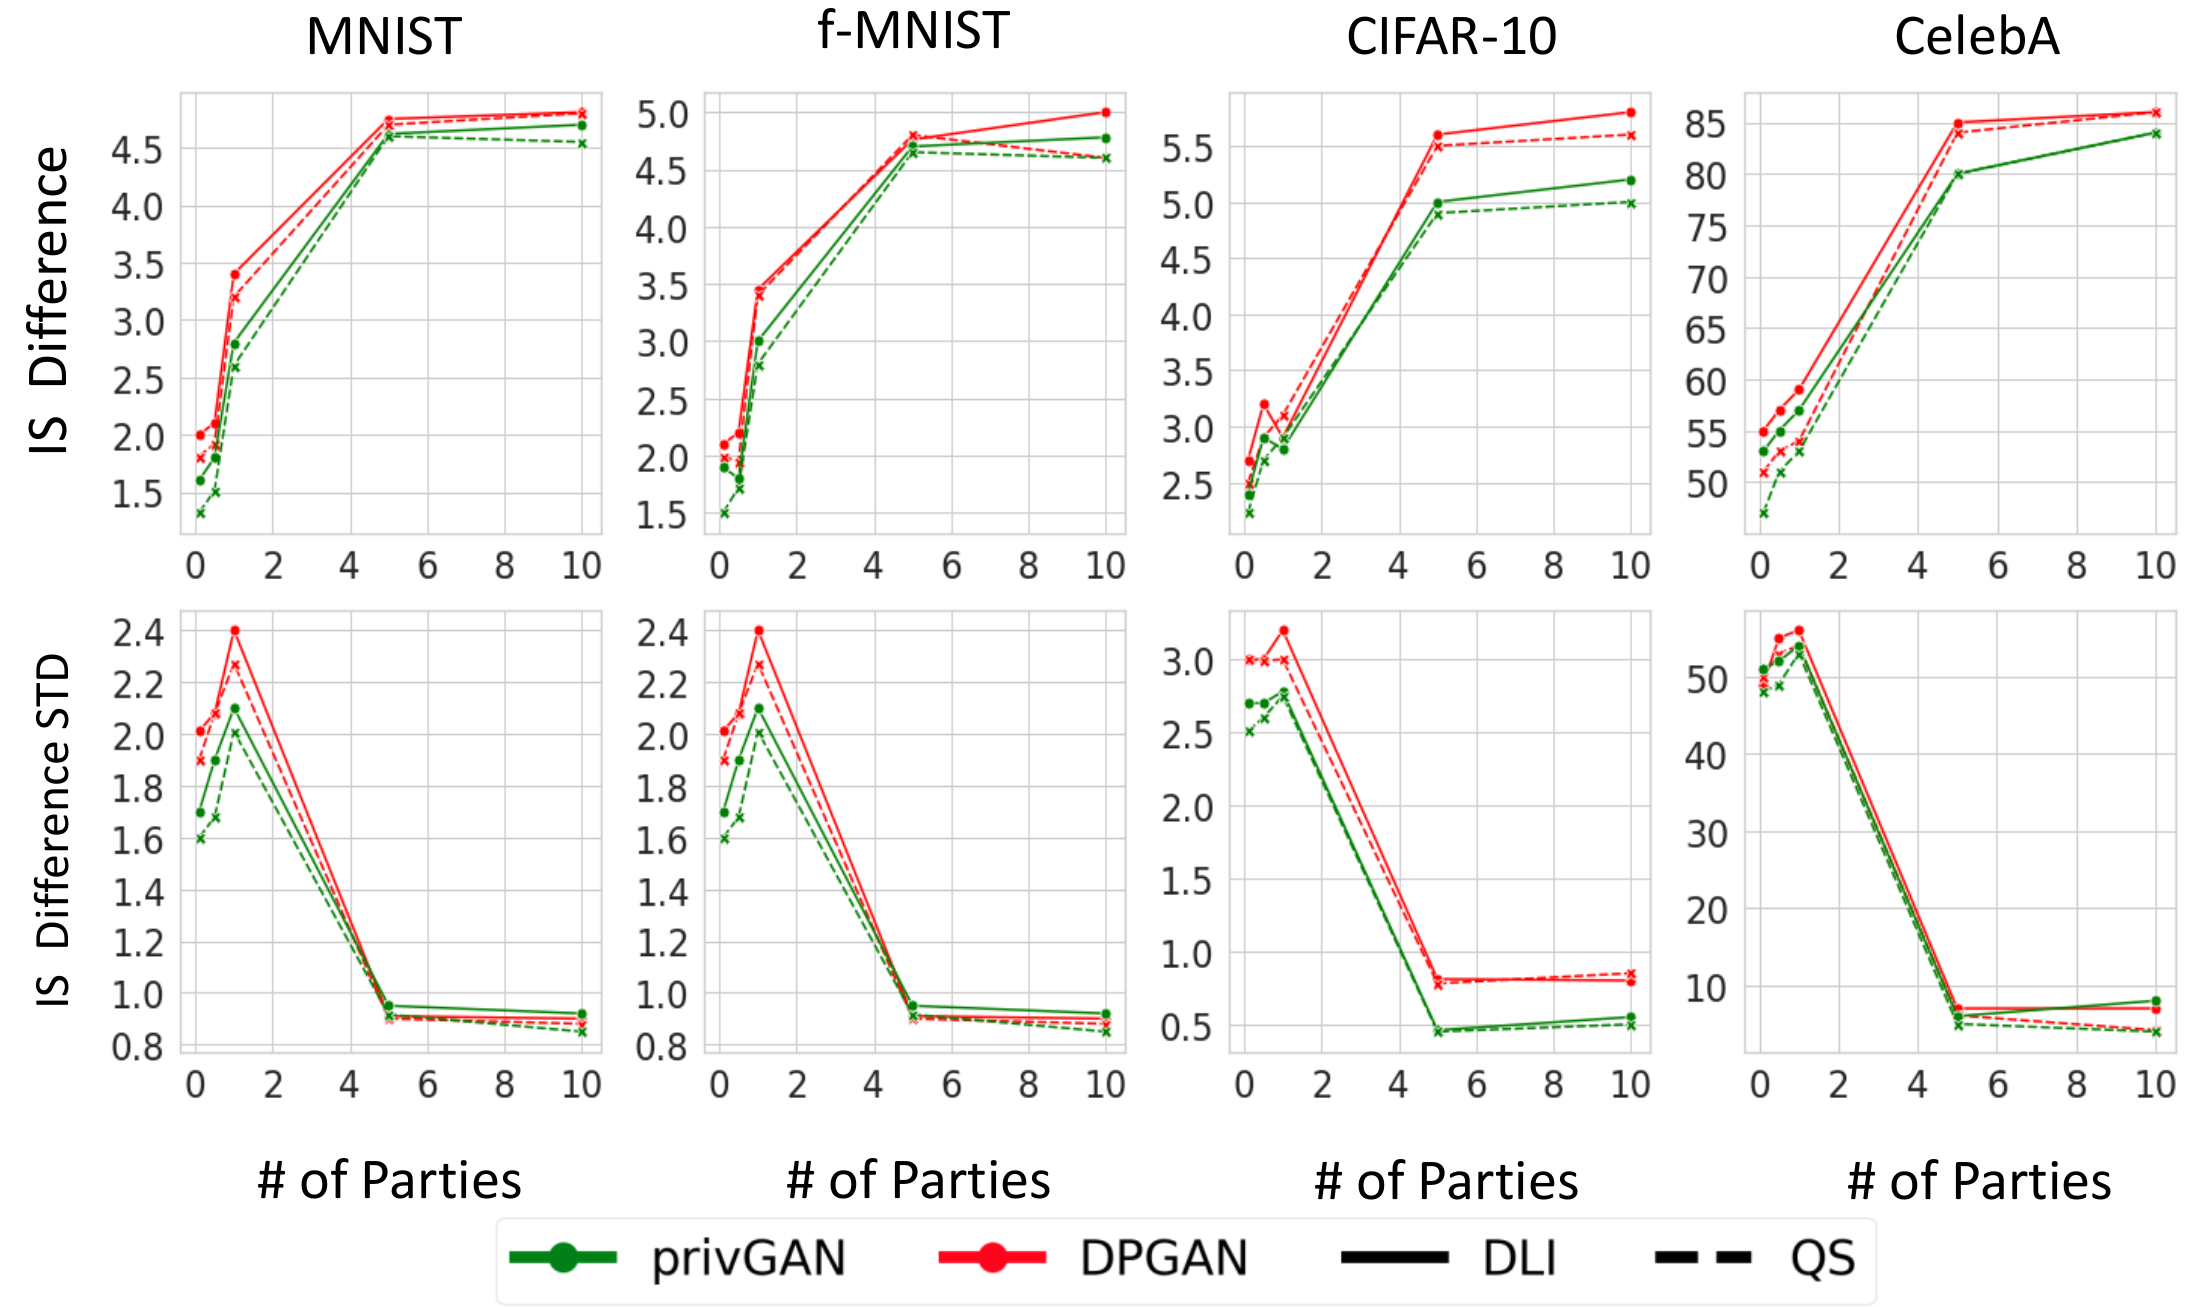
\includegraphics[width=0.8\linewidth]{Plots/IS_difference_local_gans.png}
%  \caption{Varying Concentration Parameter: The Figure depicts the average and standard deviation of IS difference between real-local-data and synthetic-local-data at various concentration parameters in privGAN and DPGAN.}
%  \label{fig:IS_difference_local_gans}
% \end{figure}


% ATTACKS






\begin{figure}
 \centering
 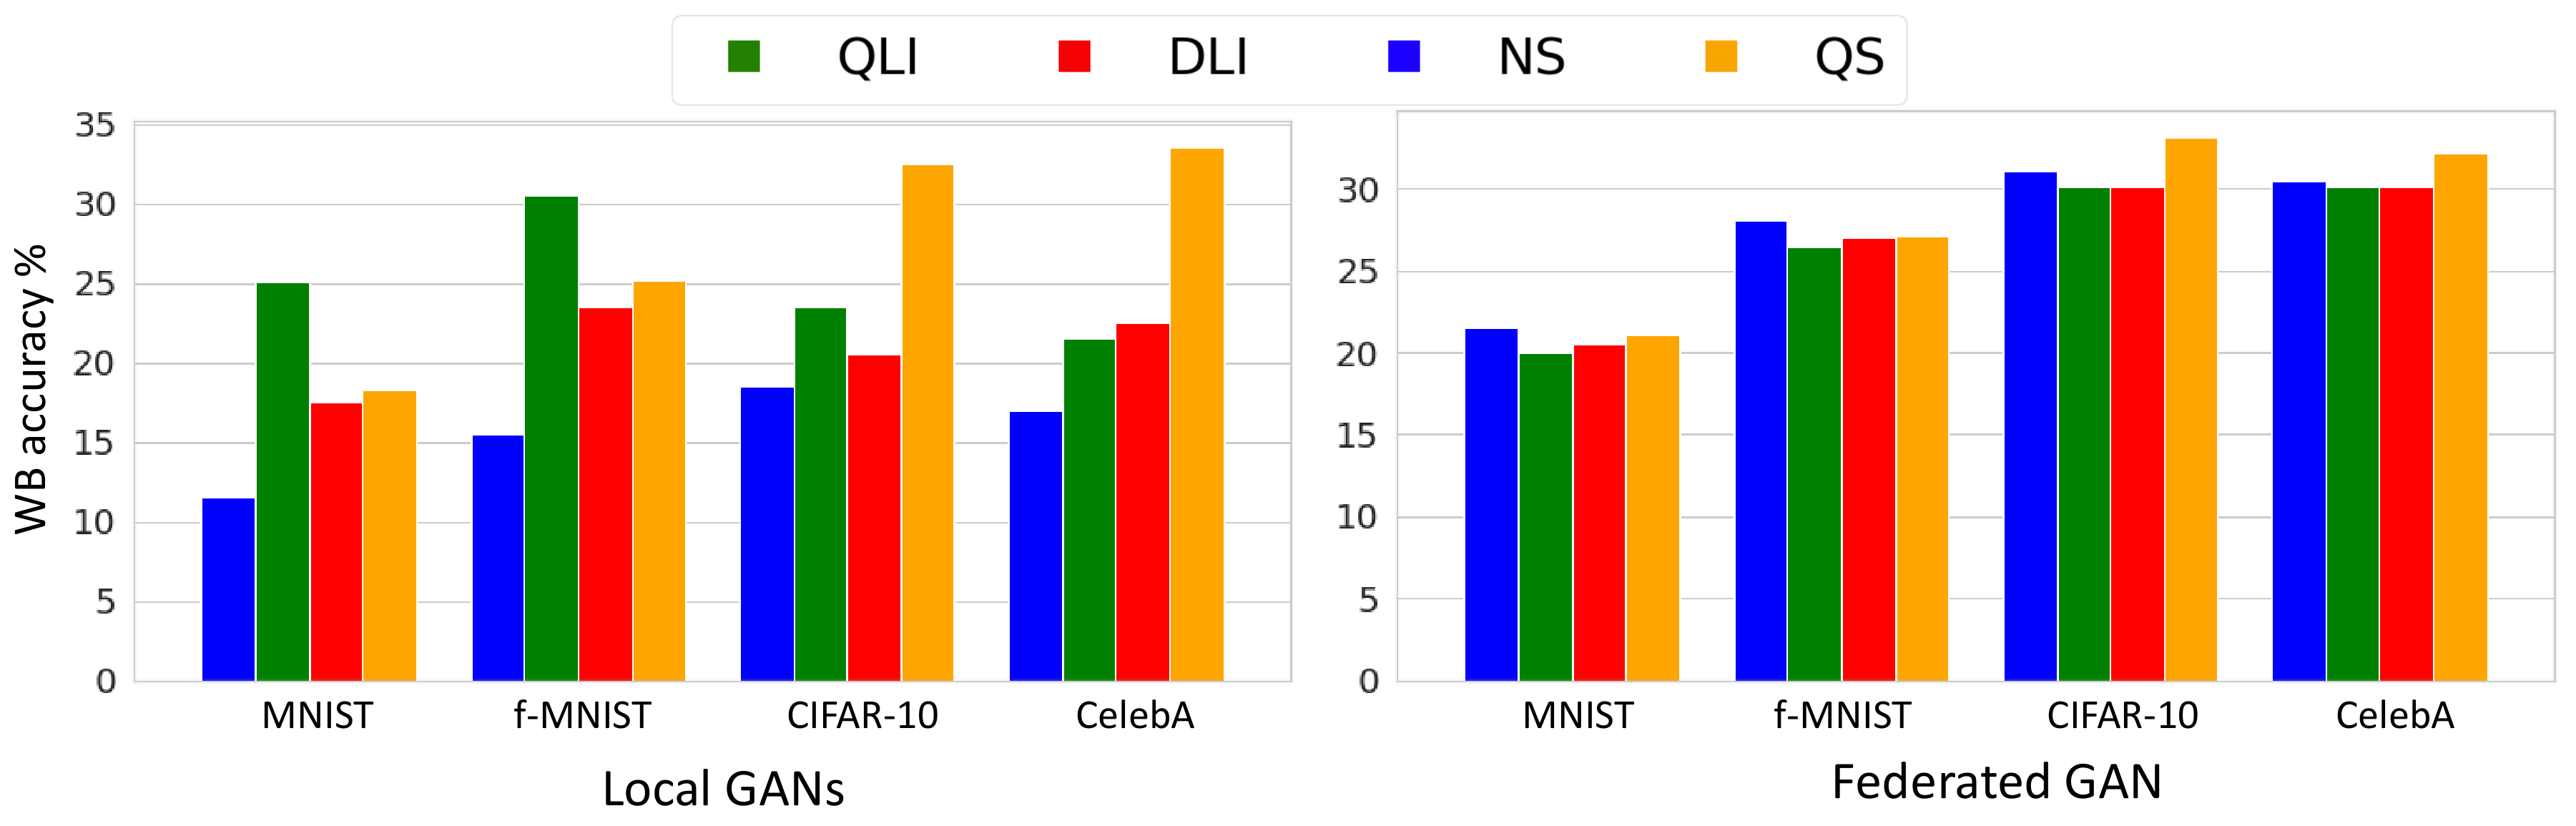
\includegraphics[width=0.7\linewidth]{Plots/baseline_WB.png}
 \caption{White-Box accuracy for Non-Private Local GANs and Federated GAN: The Figure displays the results of a white-box attack using non-private local GANs and federated GAN with $K=10$ for various distributions for each dataset.}
 \label{fig:baseline_WB}
\end{figure}


\begin{figure}
 \centering

  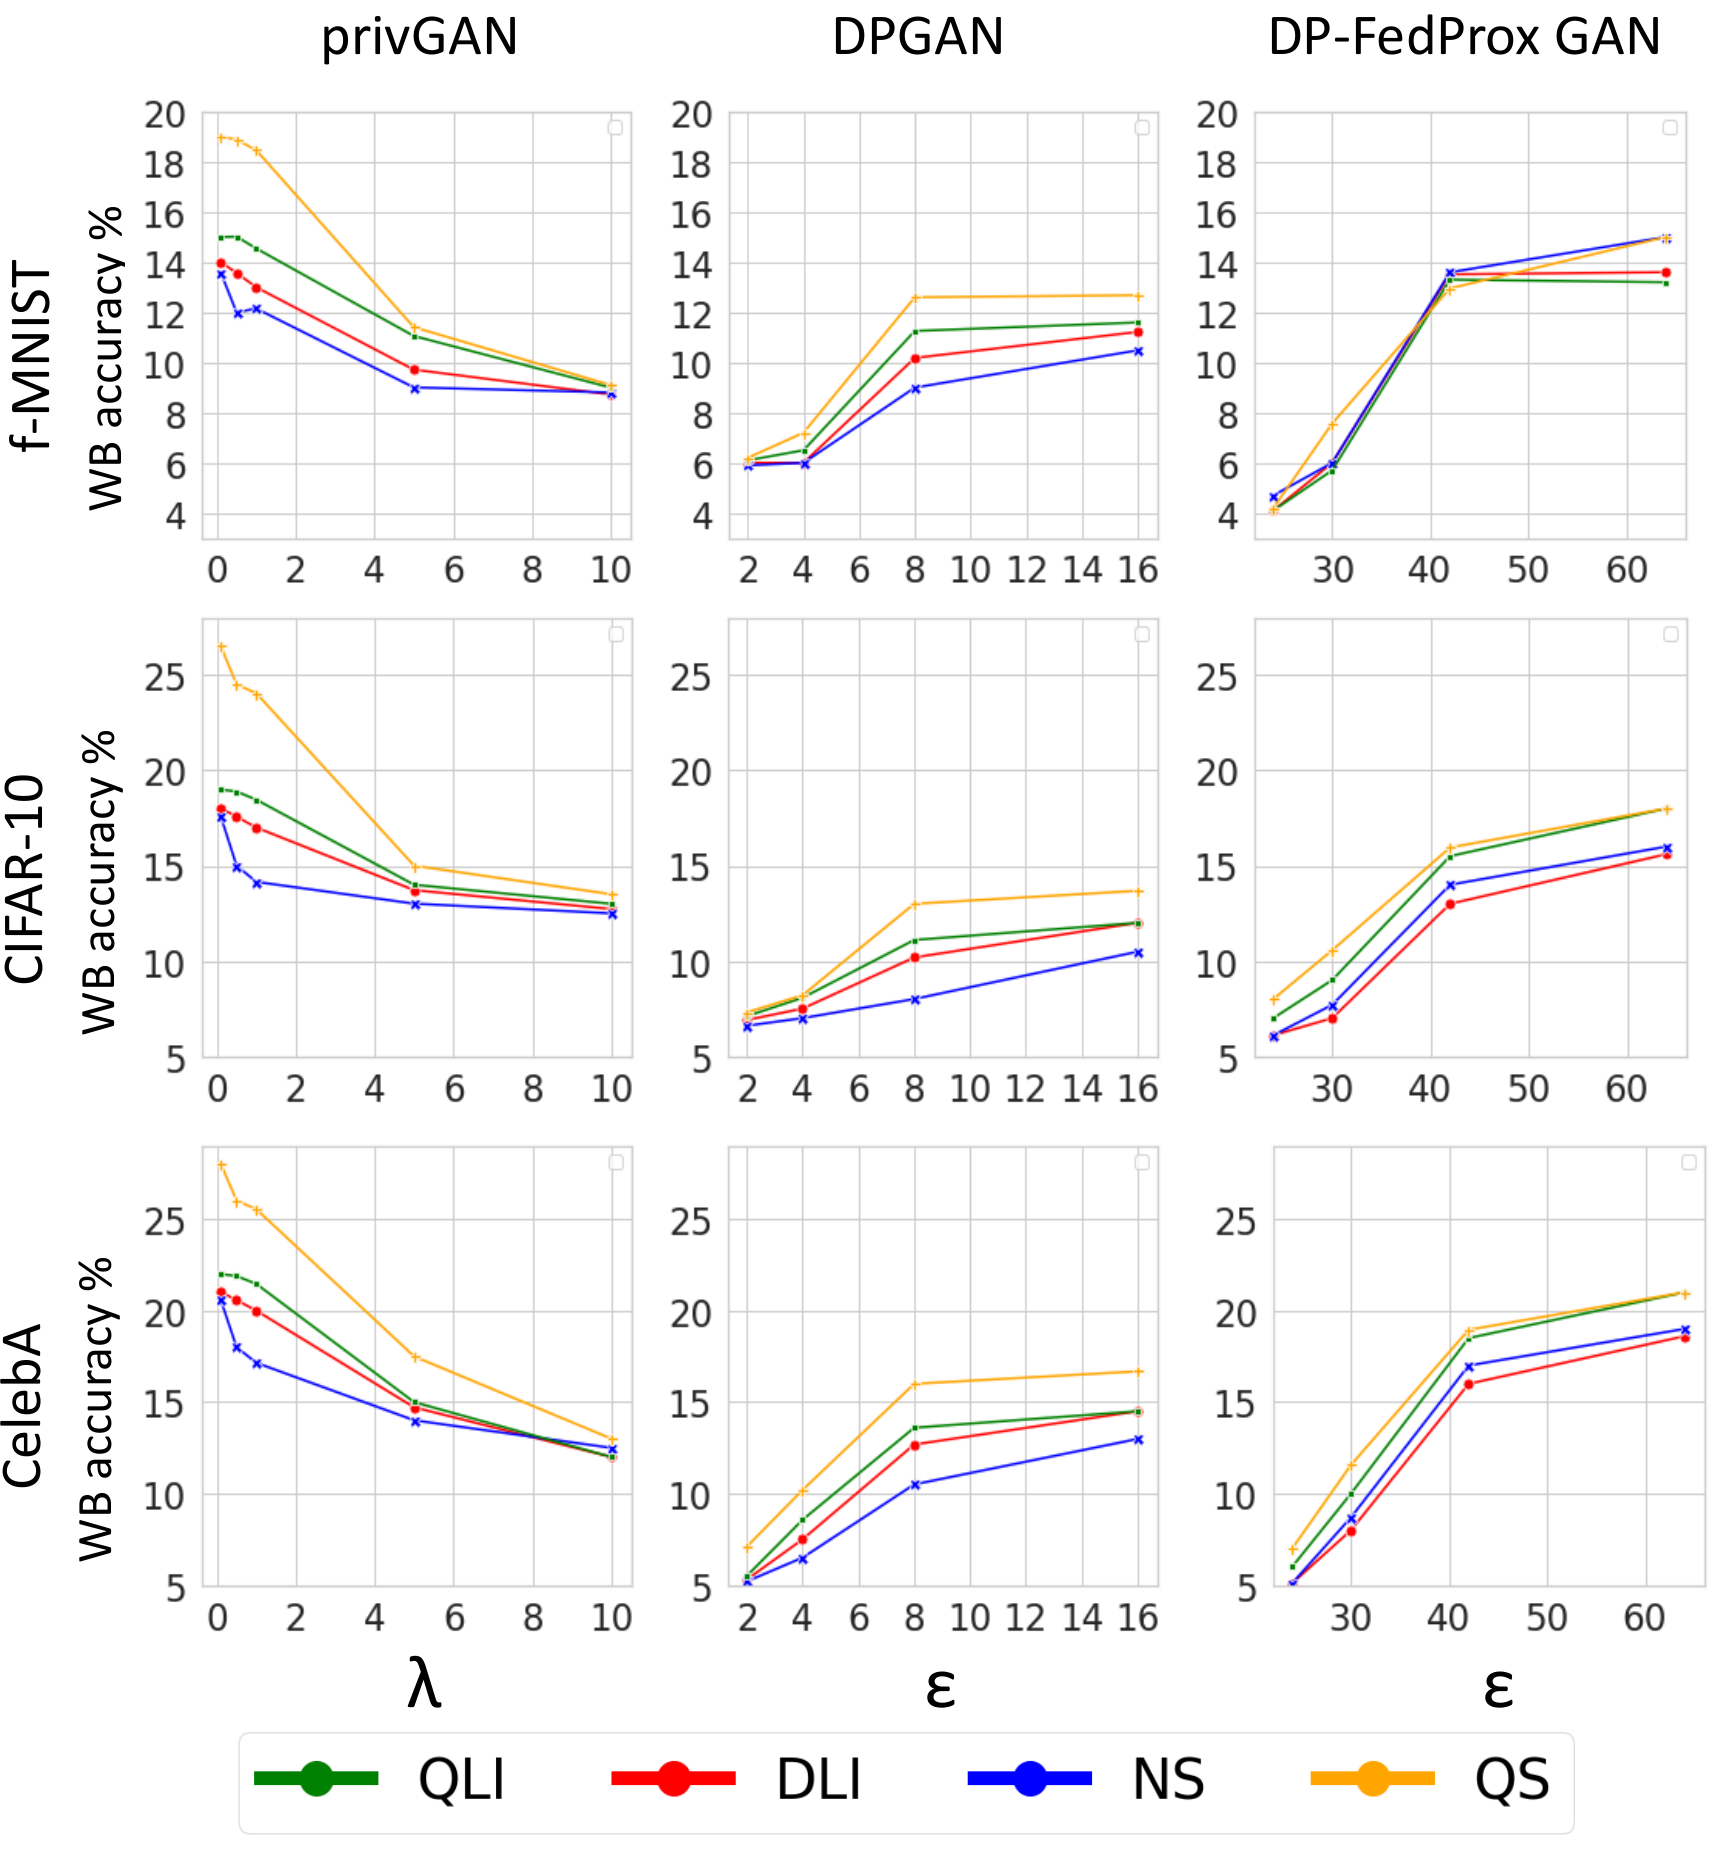
\includegraphics[width=0.6\linewidth]{Plots/vary_privacy_WB.png}

 \caption{Varying privacy parameters for White-Box Attack: The Figure shows white-box accuracy on discriminator(s) in privGAN, DPGAN, and DP-FedProx GAN for various privacy parameters.}
 \label{fig:vary_privacy_WB}
\end{figure}



\begin{figure}
 \centering
 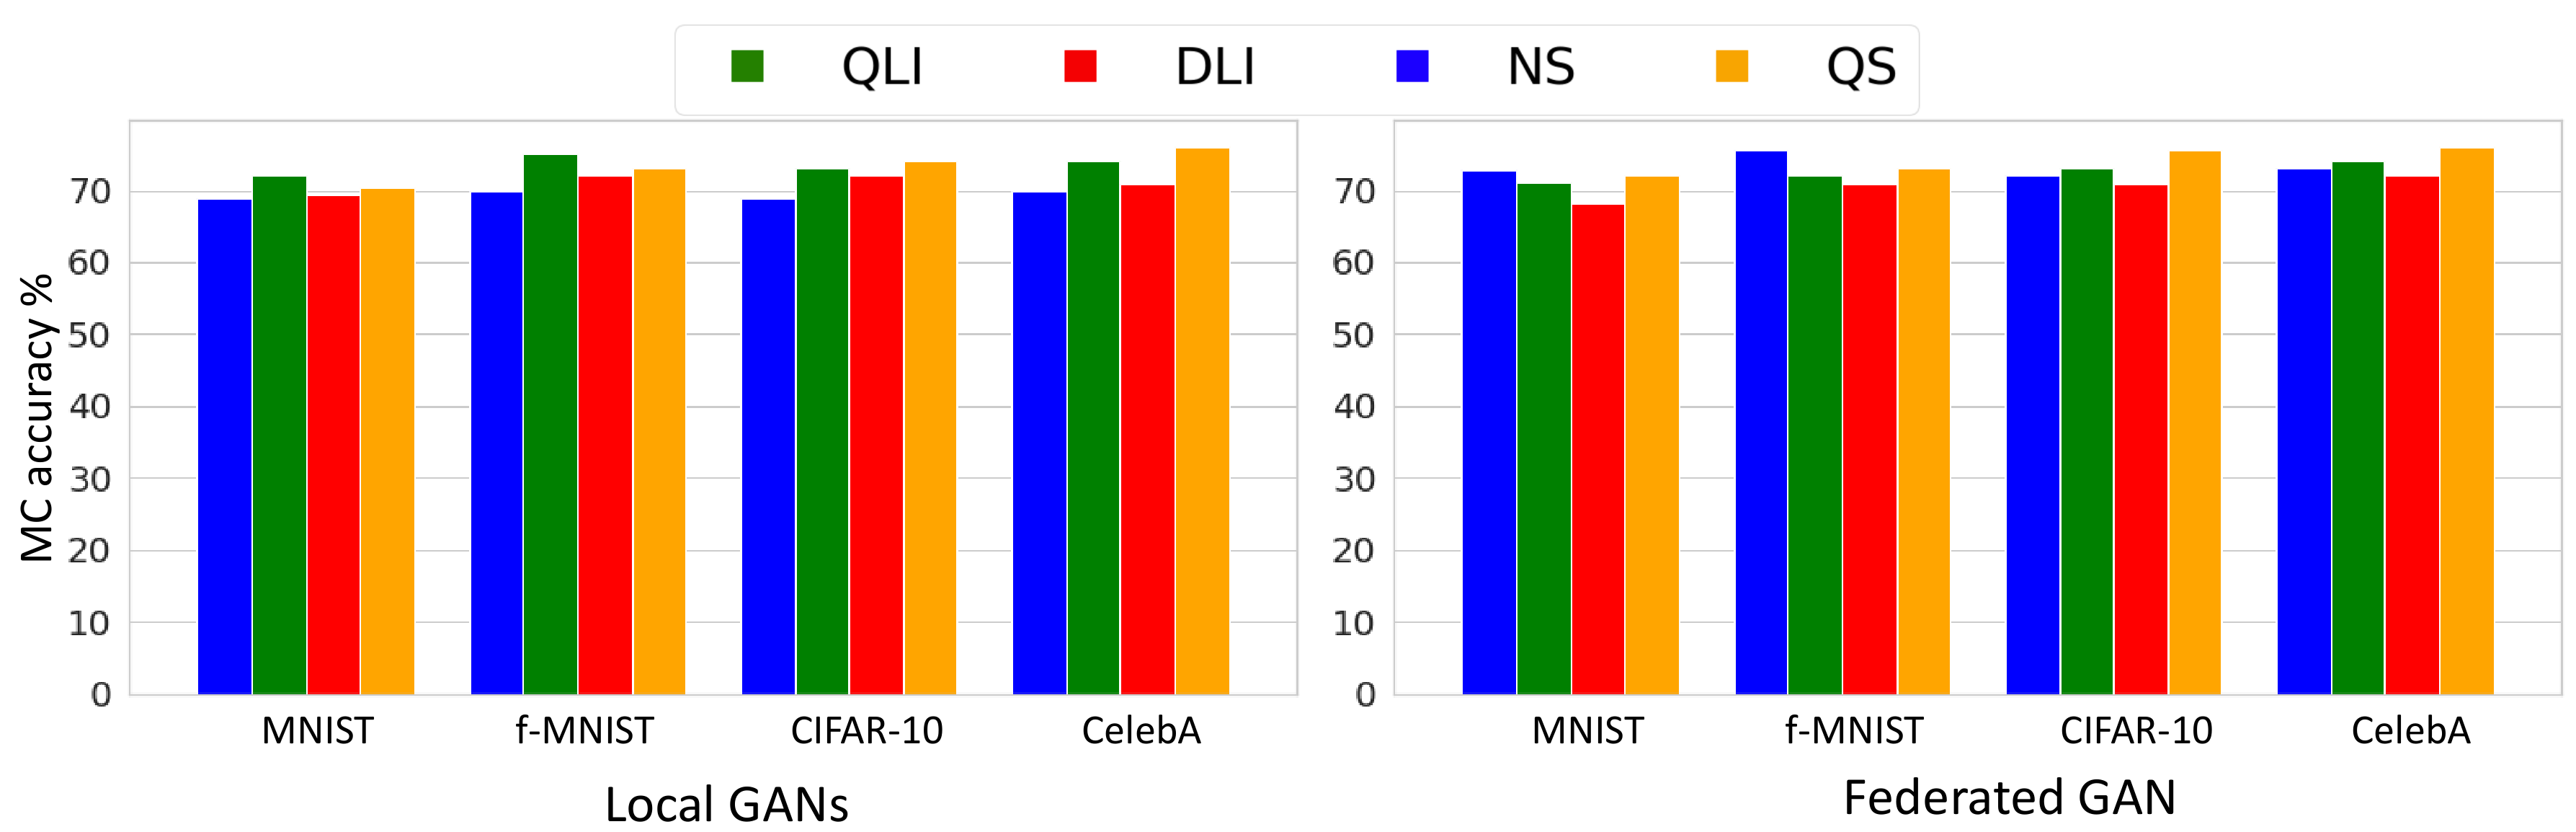
\includegraphics[width=0.7\linewidth]{Plots/MC_nonprivate.png}
 \caption{Monte-Carlo accuracy for Non-Private Local GANs and Federated GAN: The Figure displays the results of a monte-carlo attack using non-private local GANs and federated GAN with $K=10$ for various distributions for each dataset.}
 \label{fig:MC_nonprivate}
\end{figure}

\begin{figure}
 \centering
 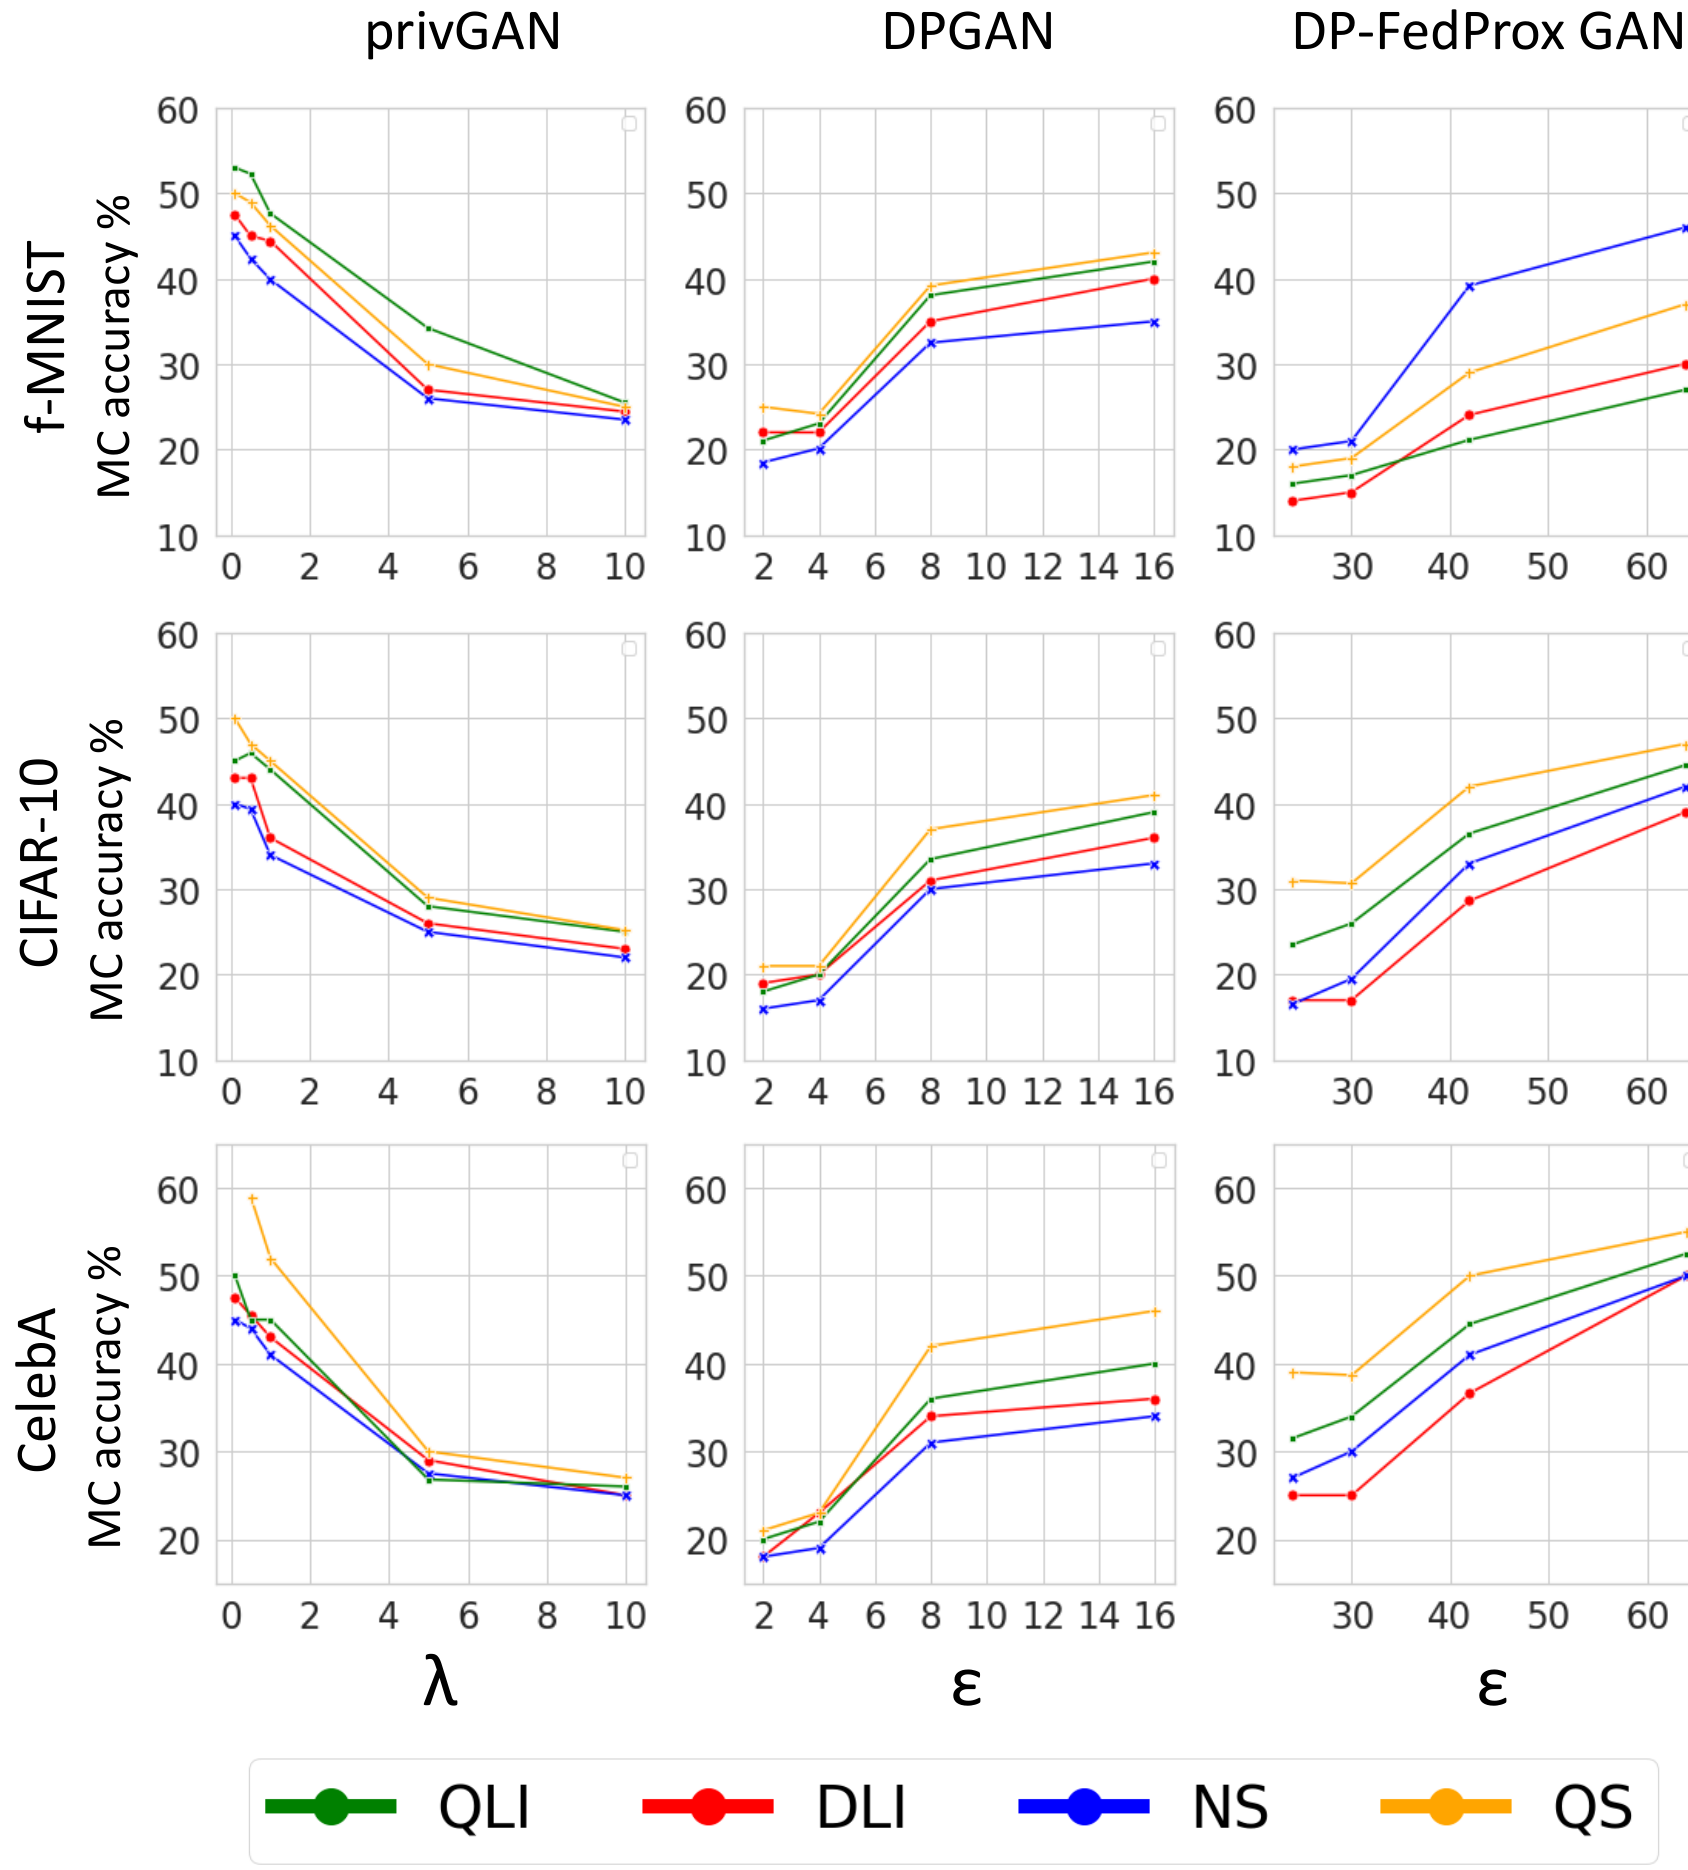
\includegraphics[width=0.6\linewidth]{Plots/vary_privacy_MC.png}
 \caption{Varying privacy parameters for Monte-Carlo Attack: The Figure shows Monte-Carlo Attack on the generator(s) in privGAN, DPGAN, and DP-FedProx GAN for various privacy parameters. }
 \label{fig:vary_privacy_MC}
\end{figure}


\begin{figure}
 \centering
 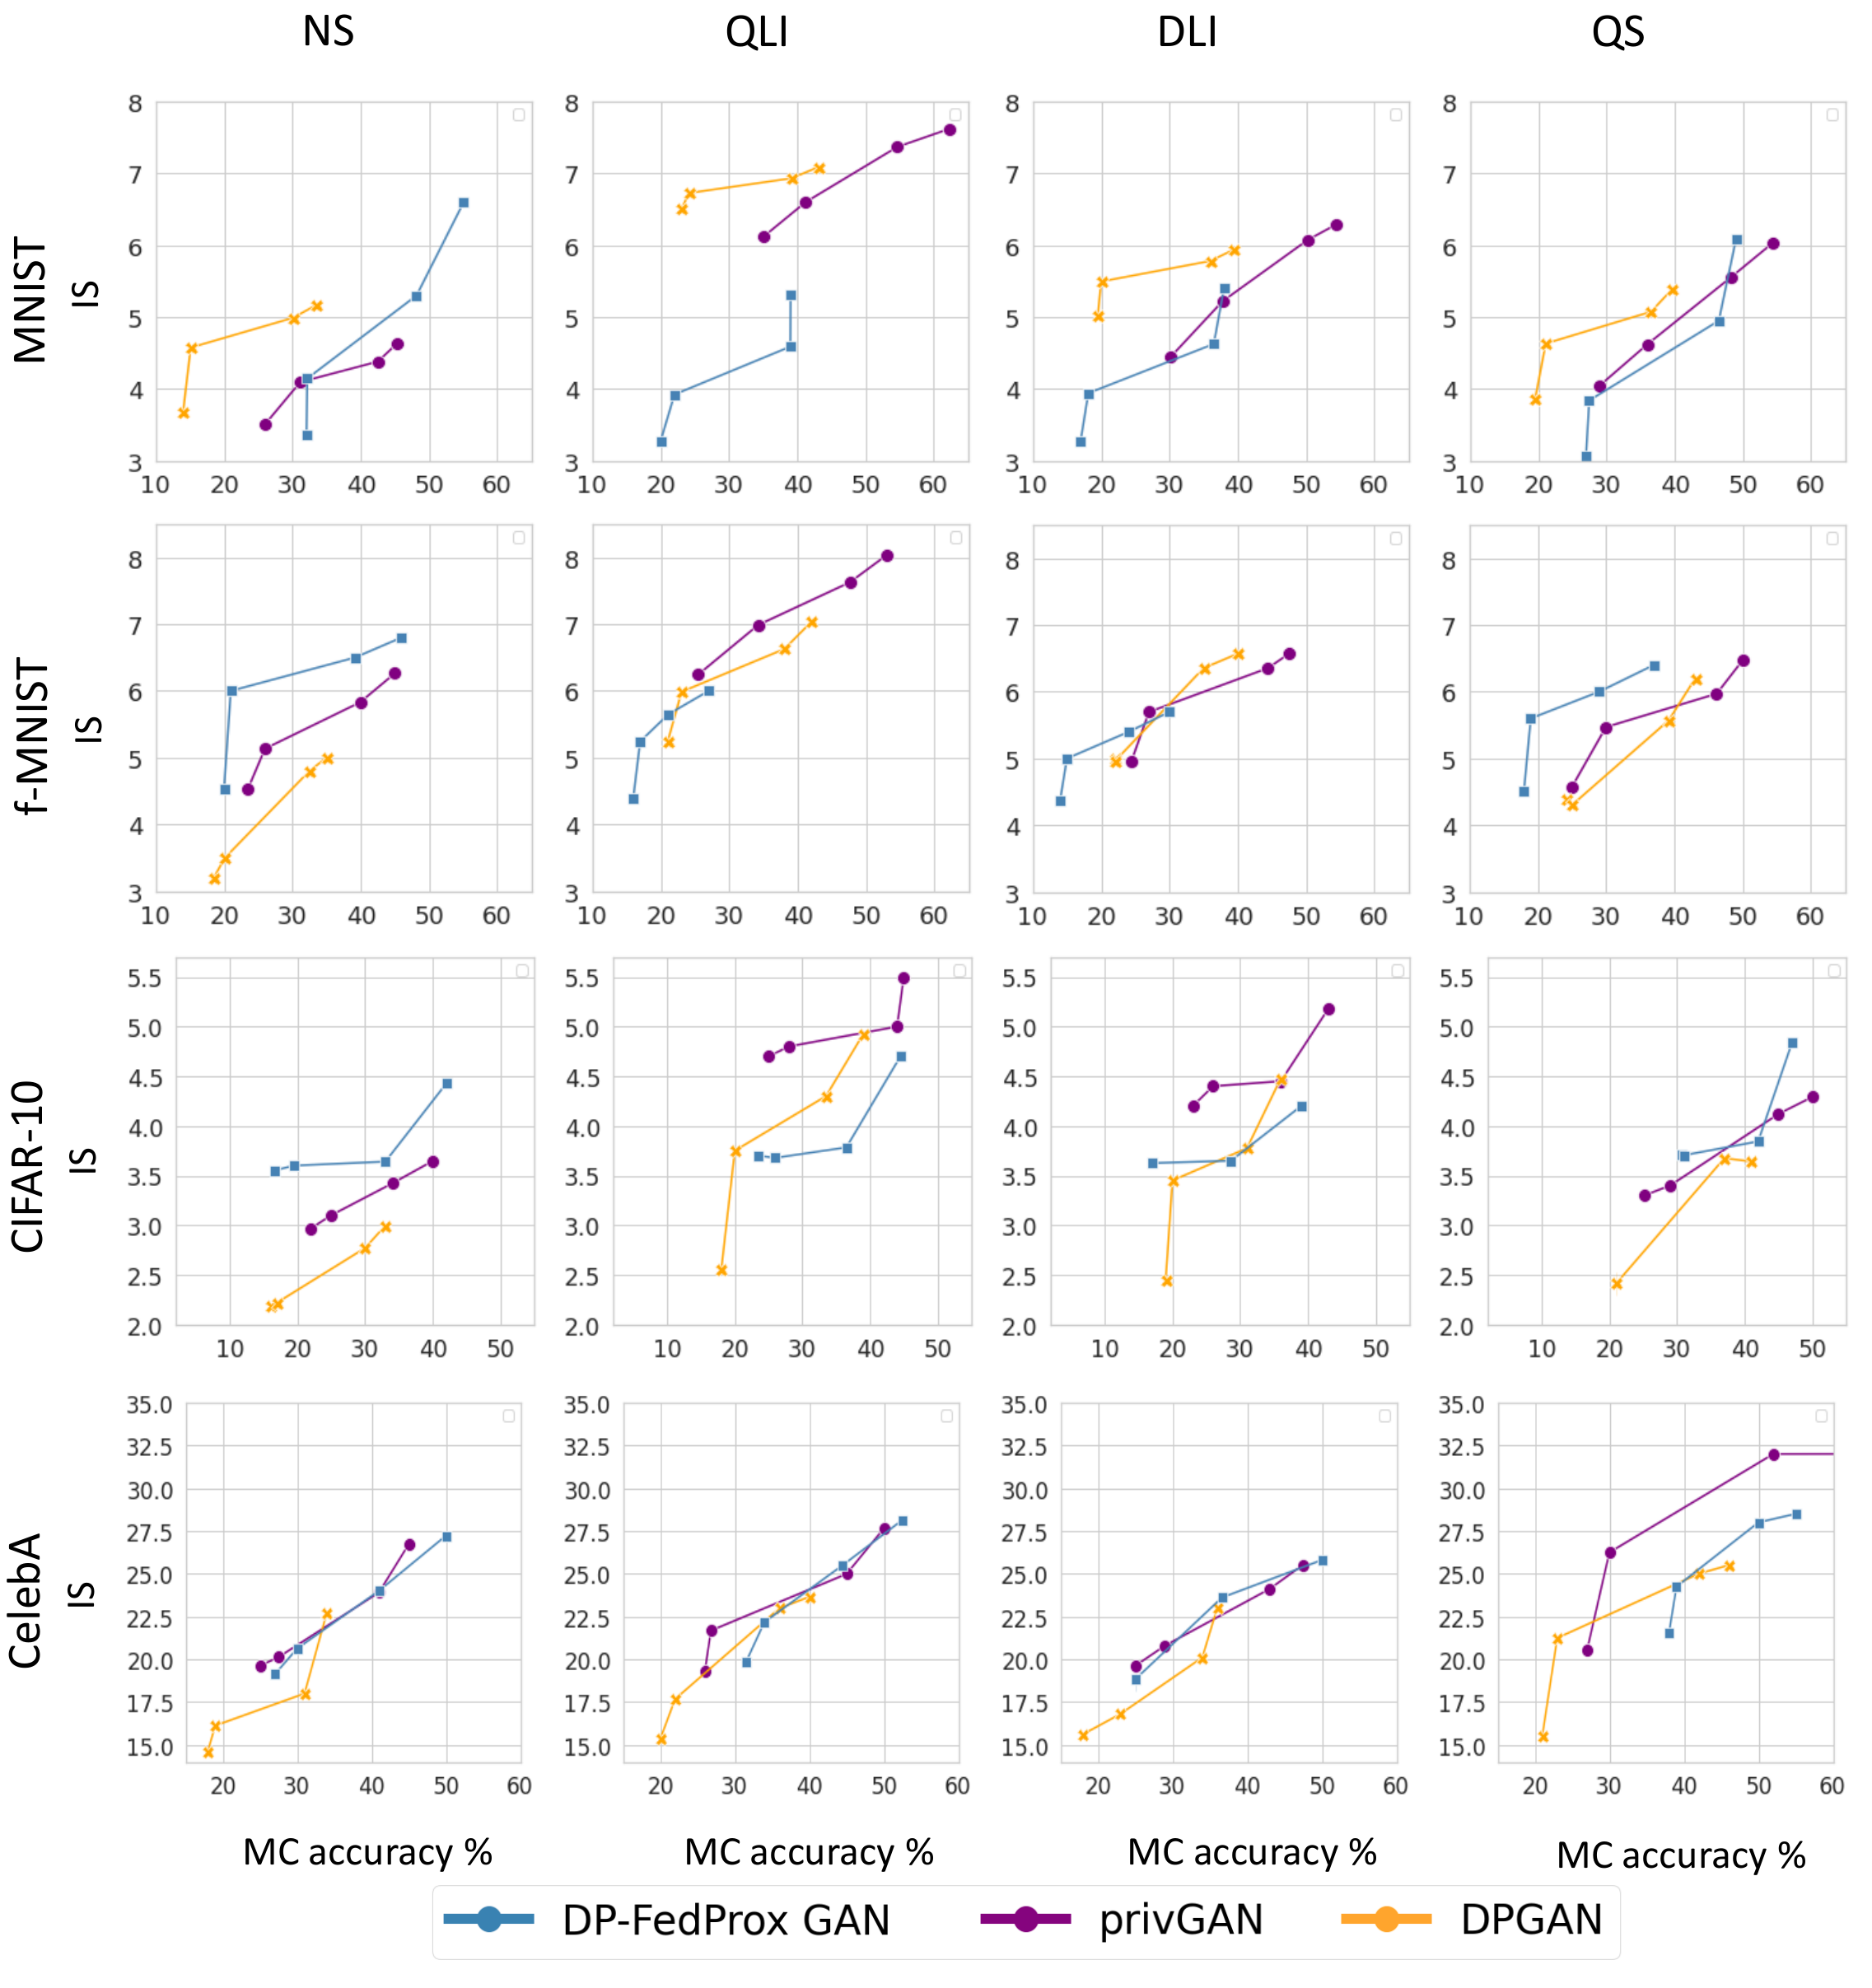
\includegraphics[width=0.8\linewidth]{Plots/varyPrivacy_MC_IS.png}
 \caption{Privacy vs. Utility: The Figure shows Monte-Carlo Attack vs Inception Score in privGAN, DPGAN, and DP-FedProx GAN for various privacy parameters.}
 \label{fig:varyPrivacy_MC_IS}
\end{figure}

\begin{figure}
 \centering
 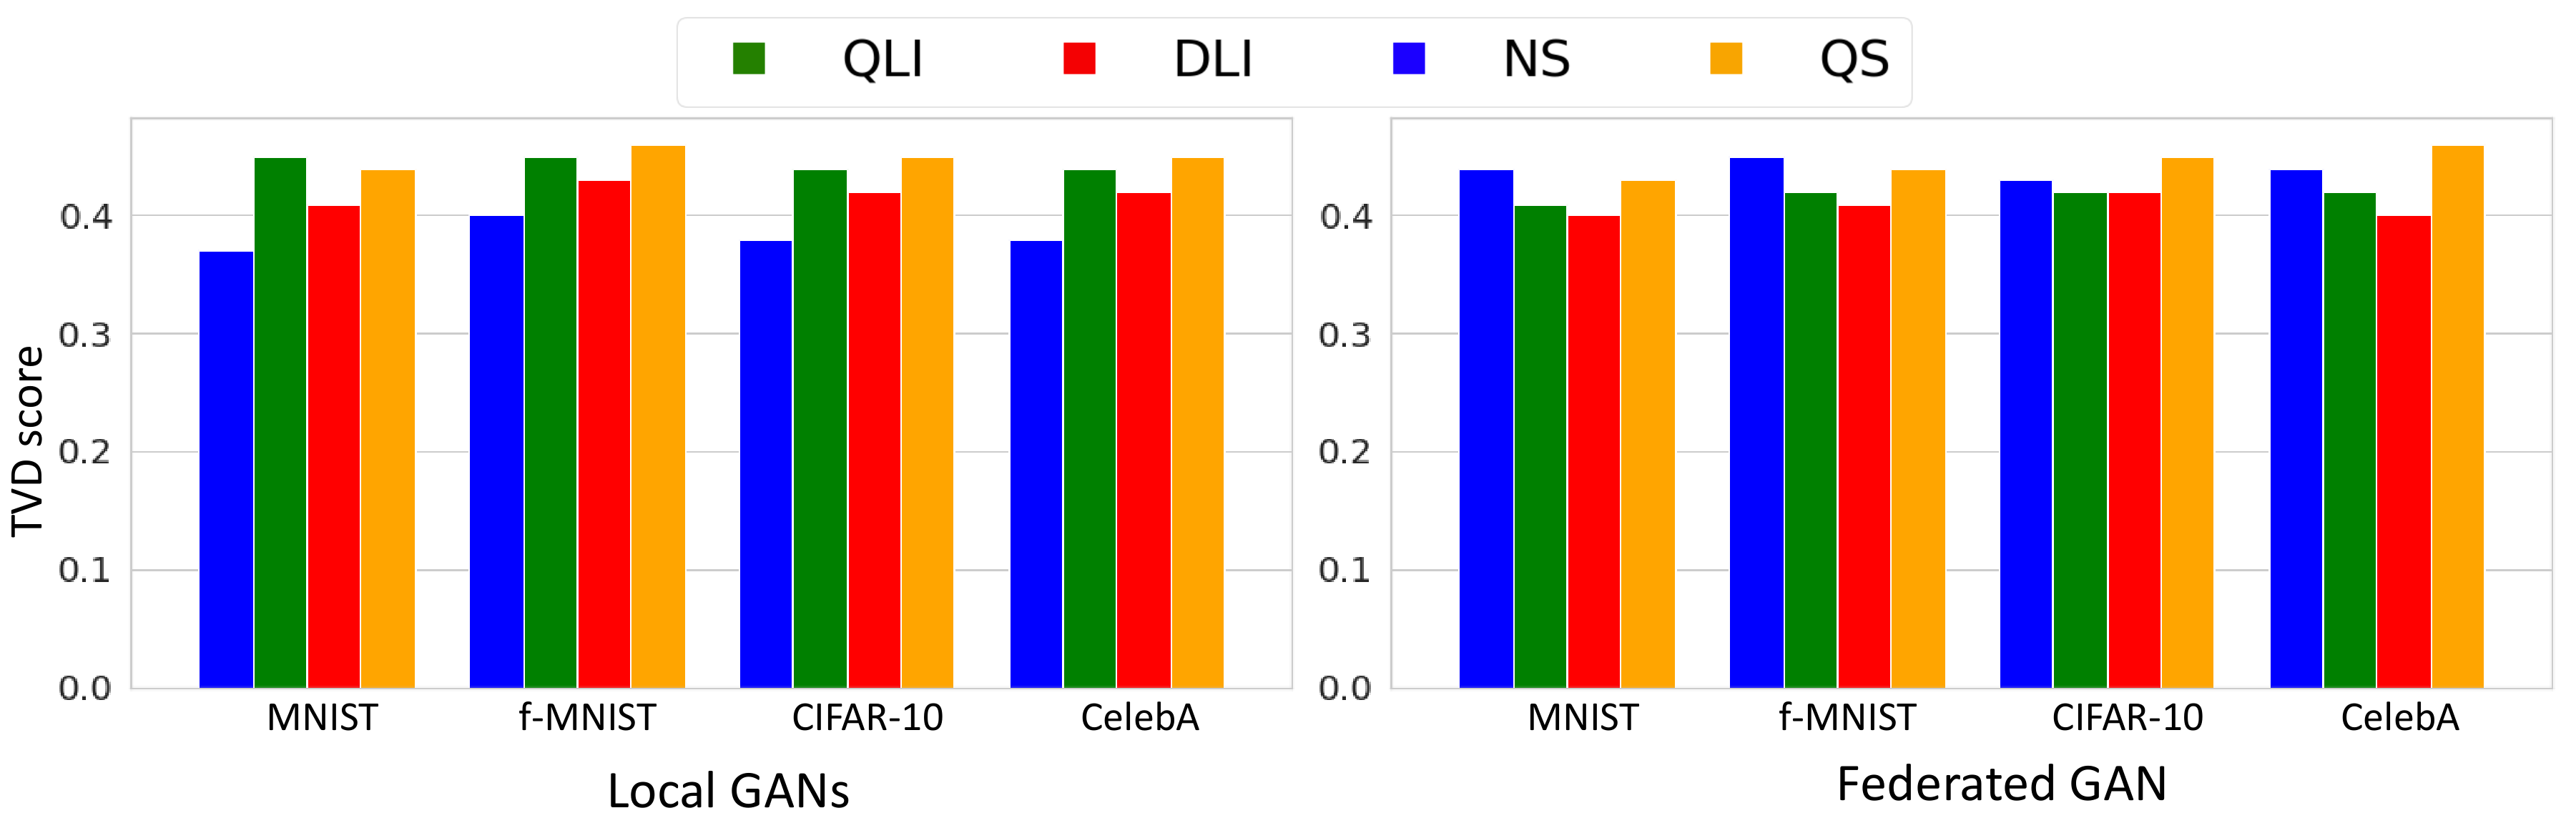
\includegraphics[width=0.7\linewidth]{Plots/TVD_nonprivate.png}
 \caption{TVD score for Non-Private Local GANs and Federated GAN: The Figure displays the results of a TVD attack score using non-private local GANs and federated GAN with $K=10$ for various distributions for each dataset.}
 \label{fig:TVD_nonprivate}
\end{figure}


\begin{figure}
 \centering
 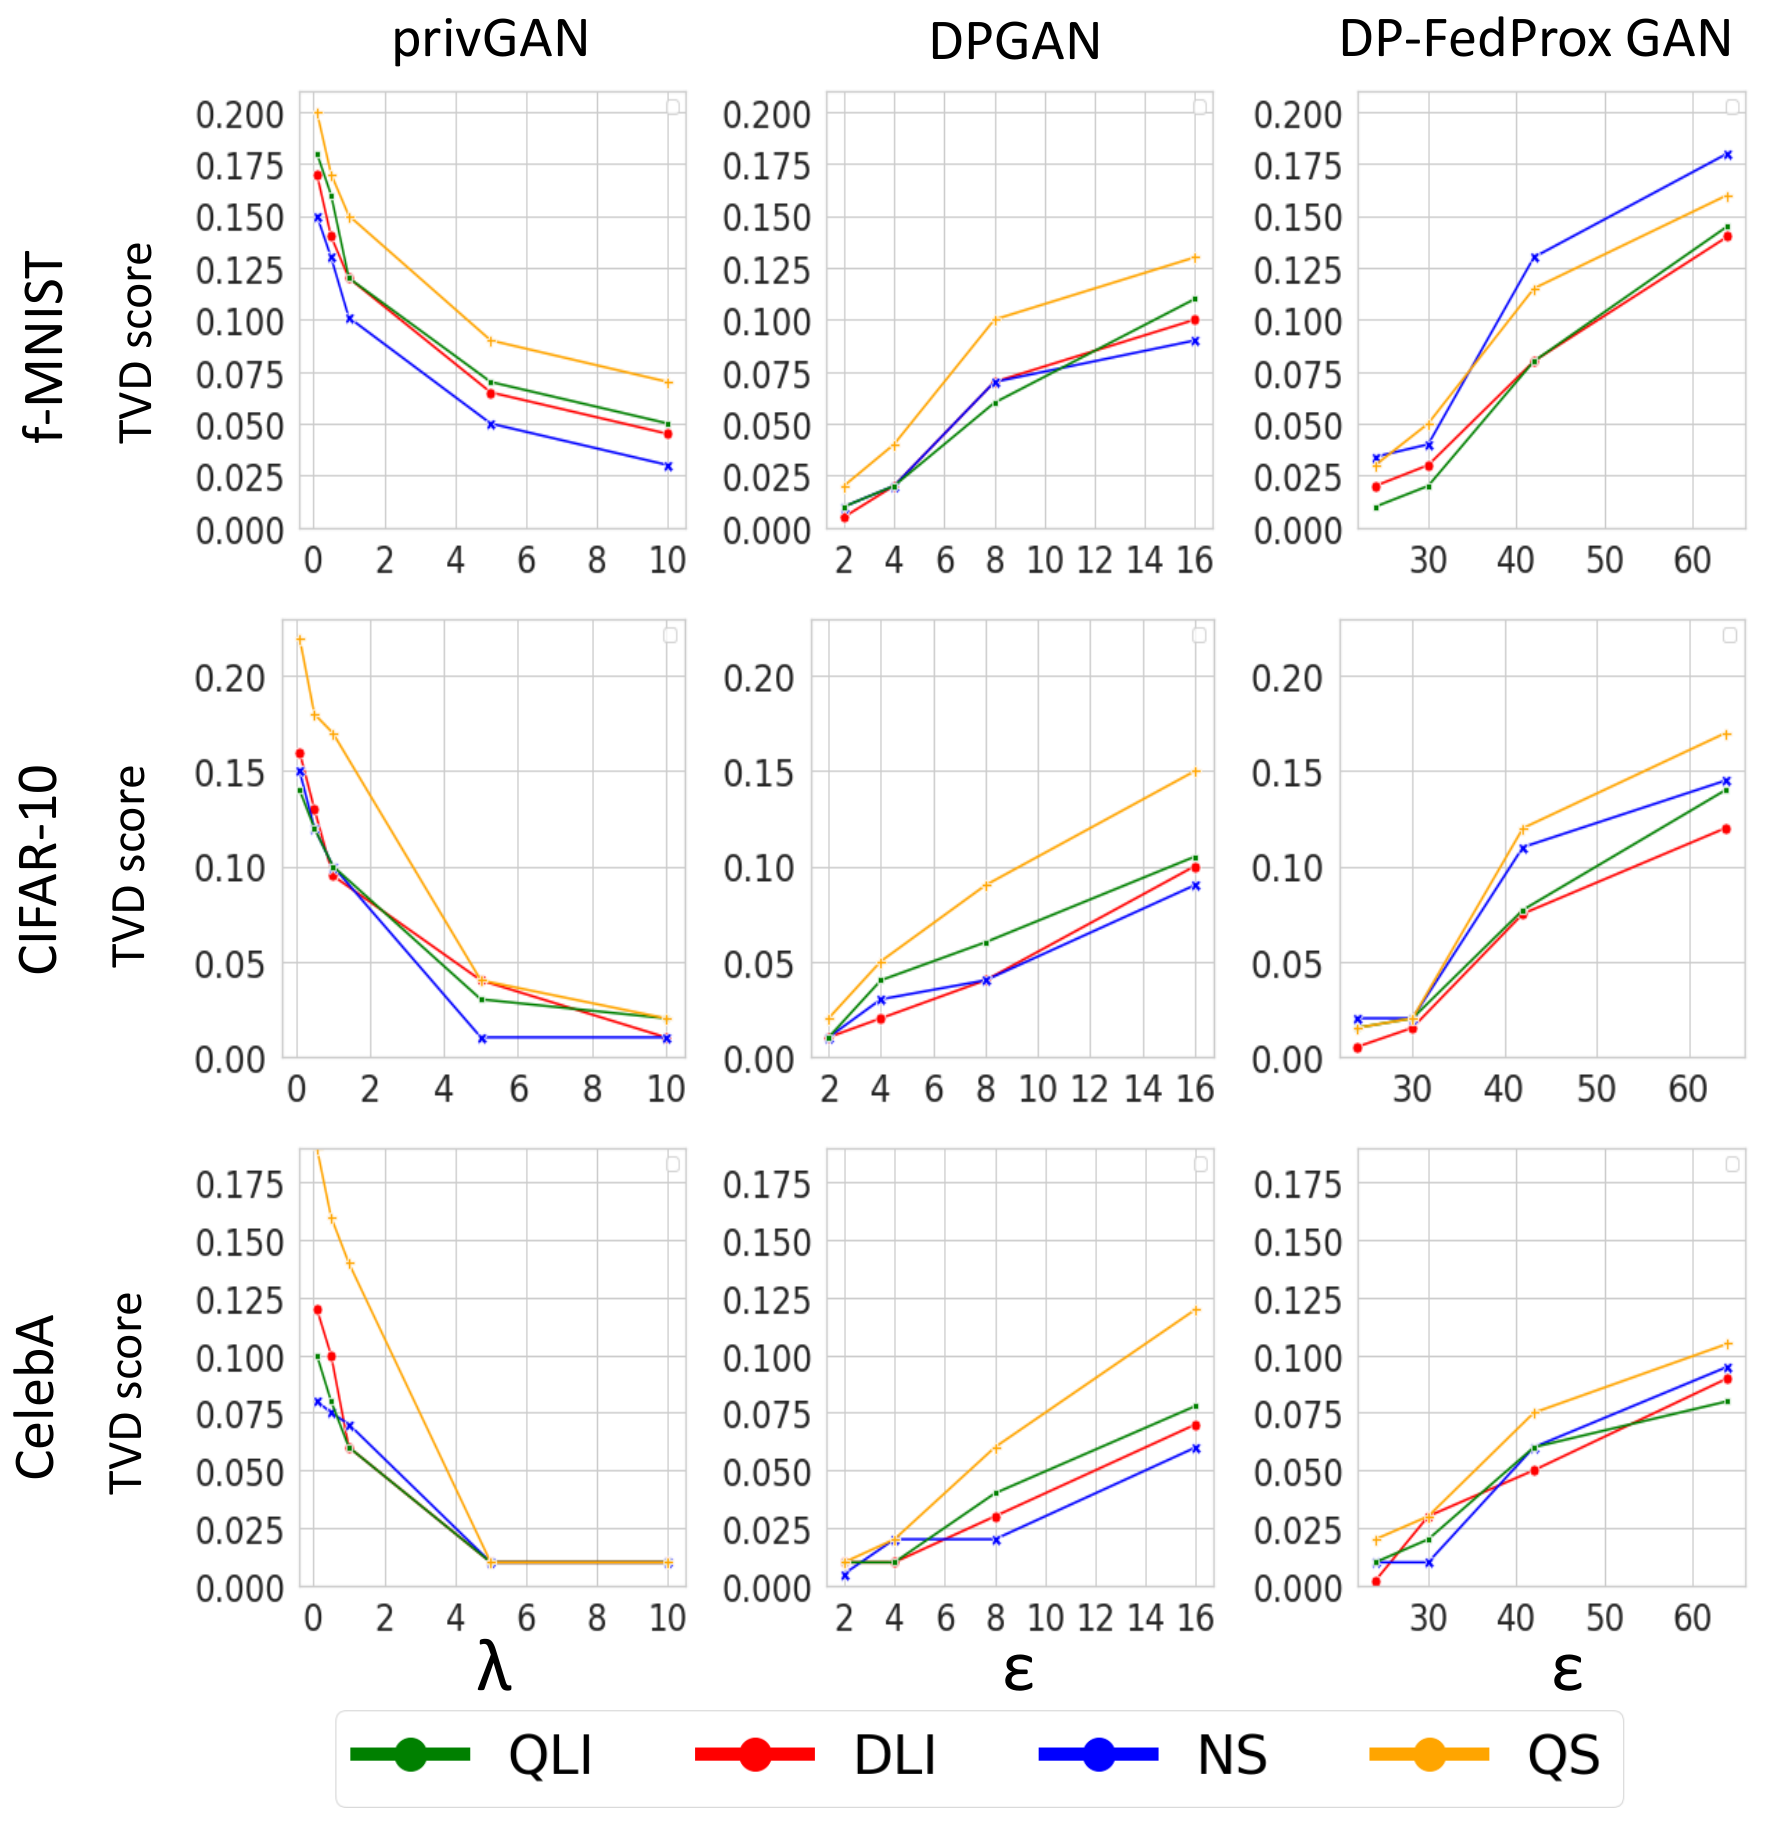
\includegraphics[width=0.6\linewidth]{Plots/vary_privacy_TVD.png}
 \caption{Varying privacy parameters for TVD Attack: For different privacy parameters, the Figure displays the TVD attack score on the discriminator(s) in privGAN, DPGAN, and DP-FedProx GAN.}
 \label{fig:vary_privacy_TVD}
\end{figure}



\begin{figure}
 \centering
 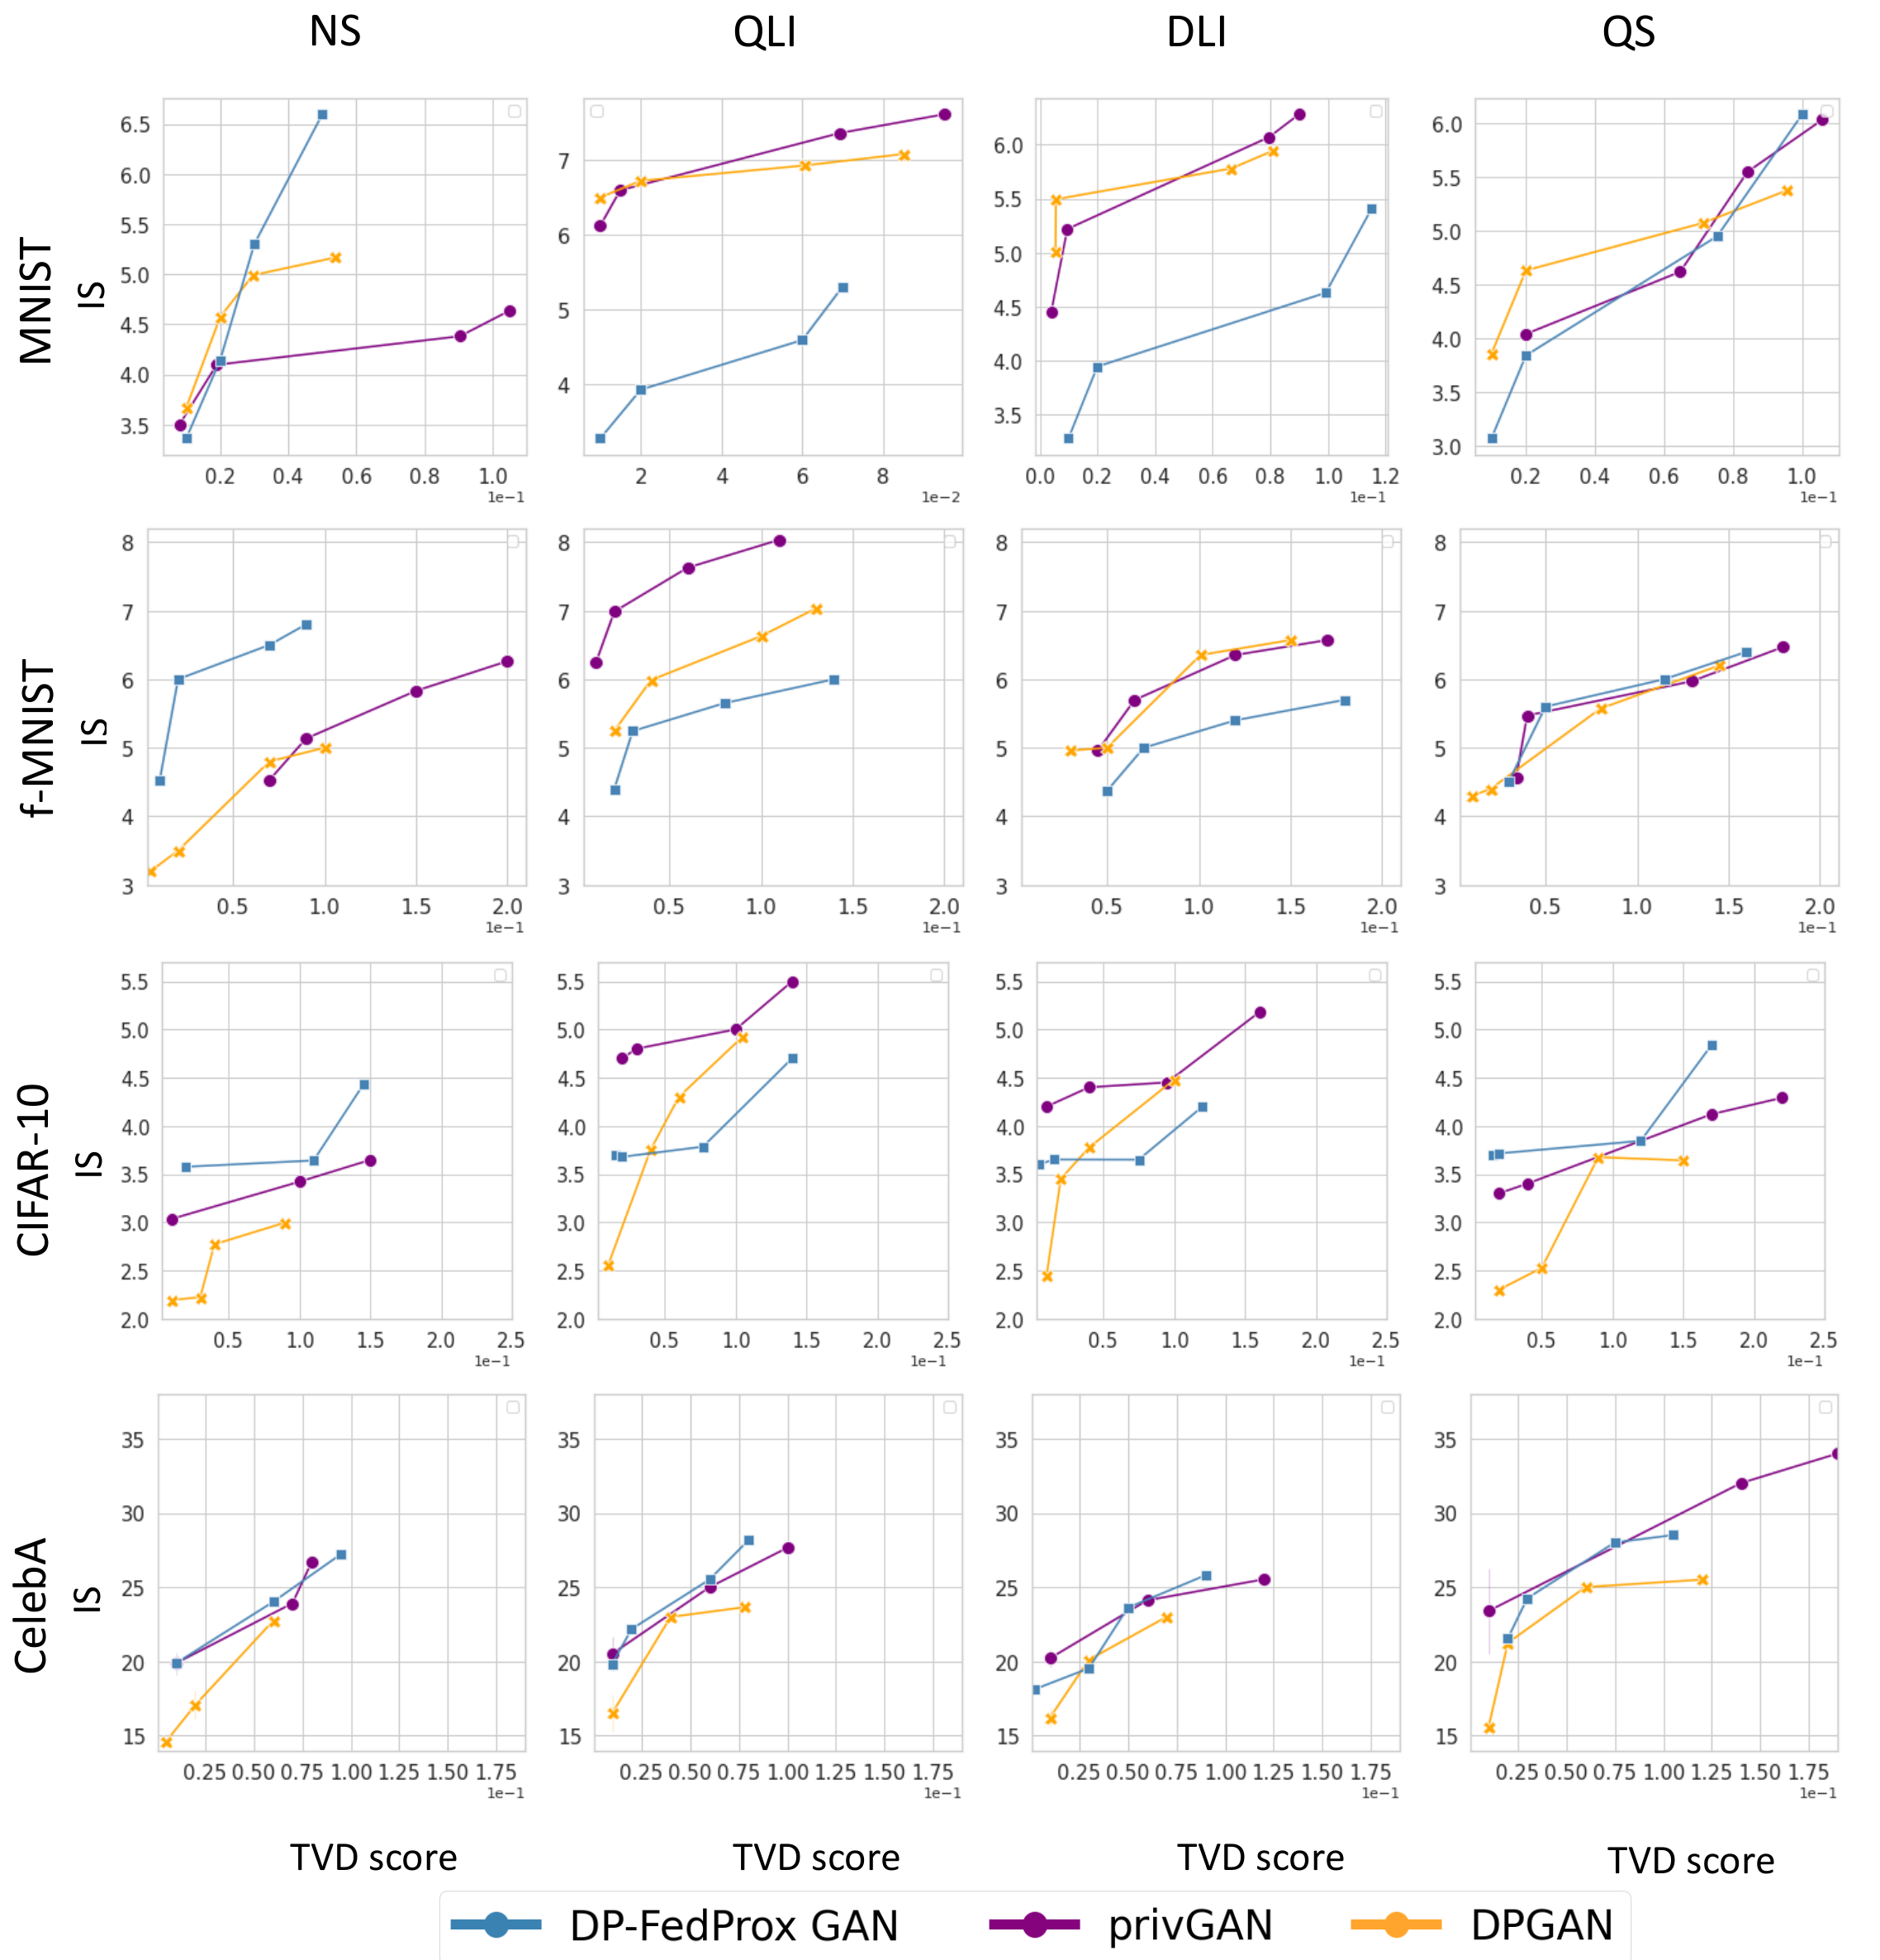
\includegraphics[width=0.8\linewidth]{Plots/varyPrivacy_TVD_IS.png}
 \caption{Privacy vs. Utility: The Figure shows TVD Attack vs Inception Score in privGAN, DPGAN, and DP-FedProx GAN for various privacy parameters.}
 \label{fig:varyPrivacy_MC_IS}
\end{figure}



% \begin{figure}
%  \centering
%  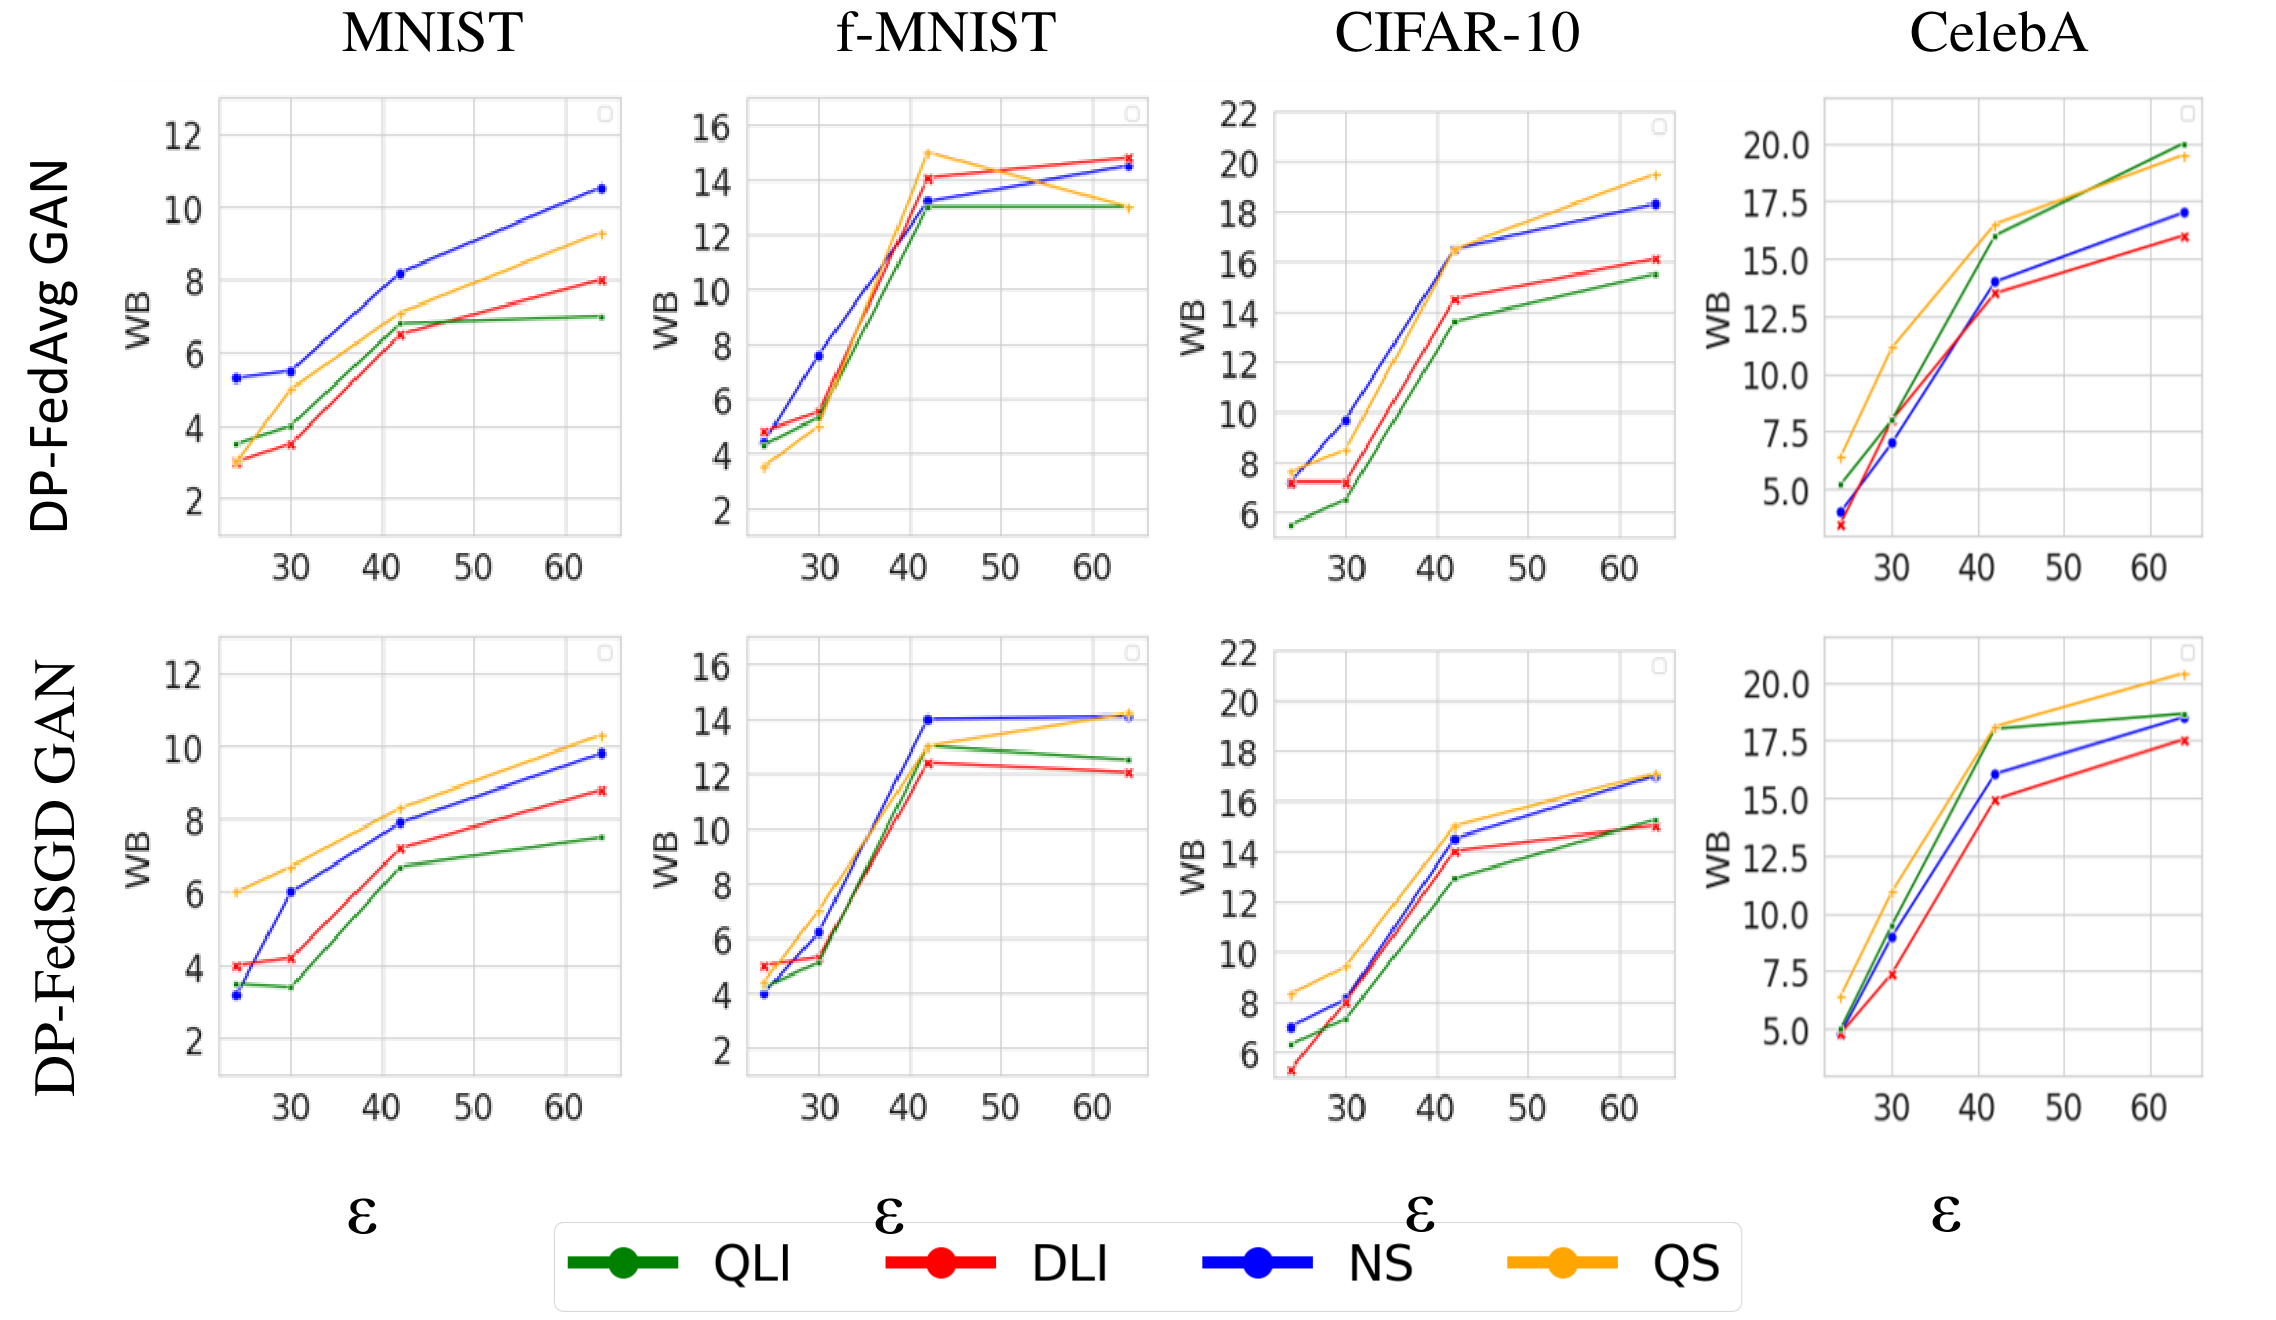
\includegraphics[width=0.8\linewidth]{Plots/vary_privacy_fedsgd_fedavg_WB.png}
%  \caption{Varying Privacy Parameters for WB-Attack: The figure shows WB Attack at various privacy parameters in DP-FedAvg GAN and DP-FedSGD GAN discriminator}
%  \label{fig:vary_privacy_fedsgd_fedavg_WB}
% \end{figure}


% \begin{figure}
%  \centering
%  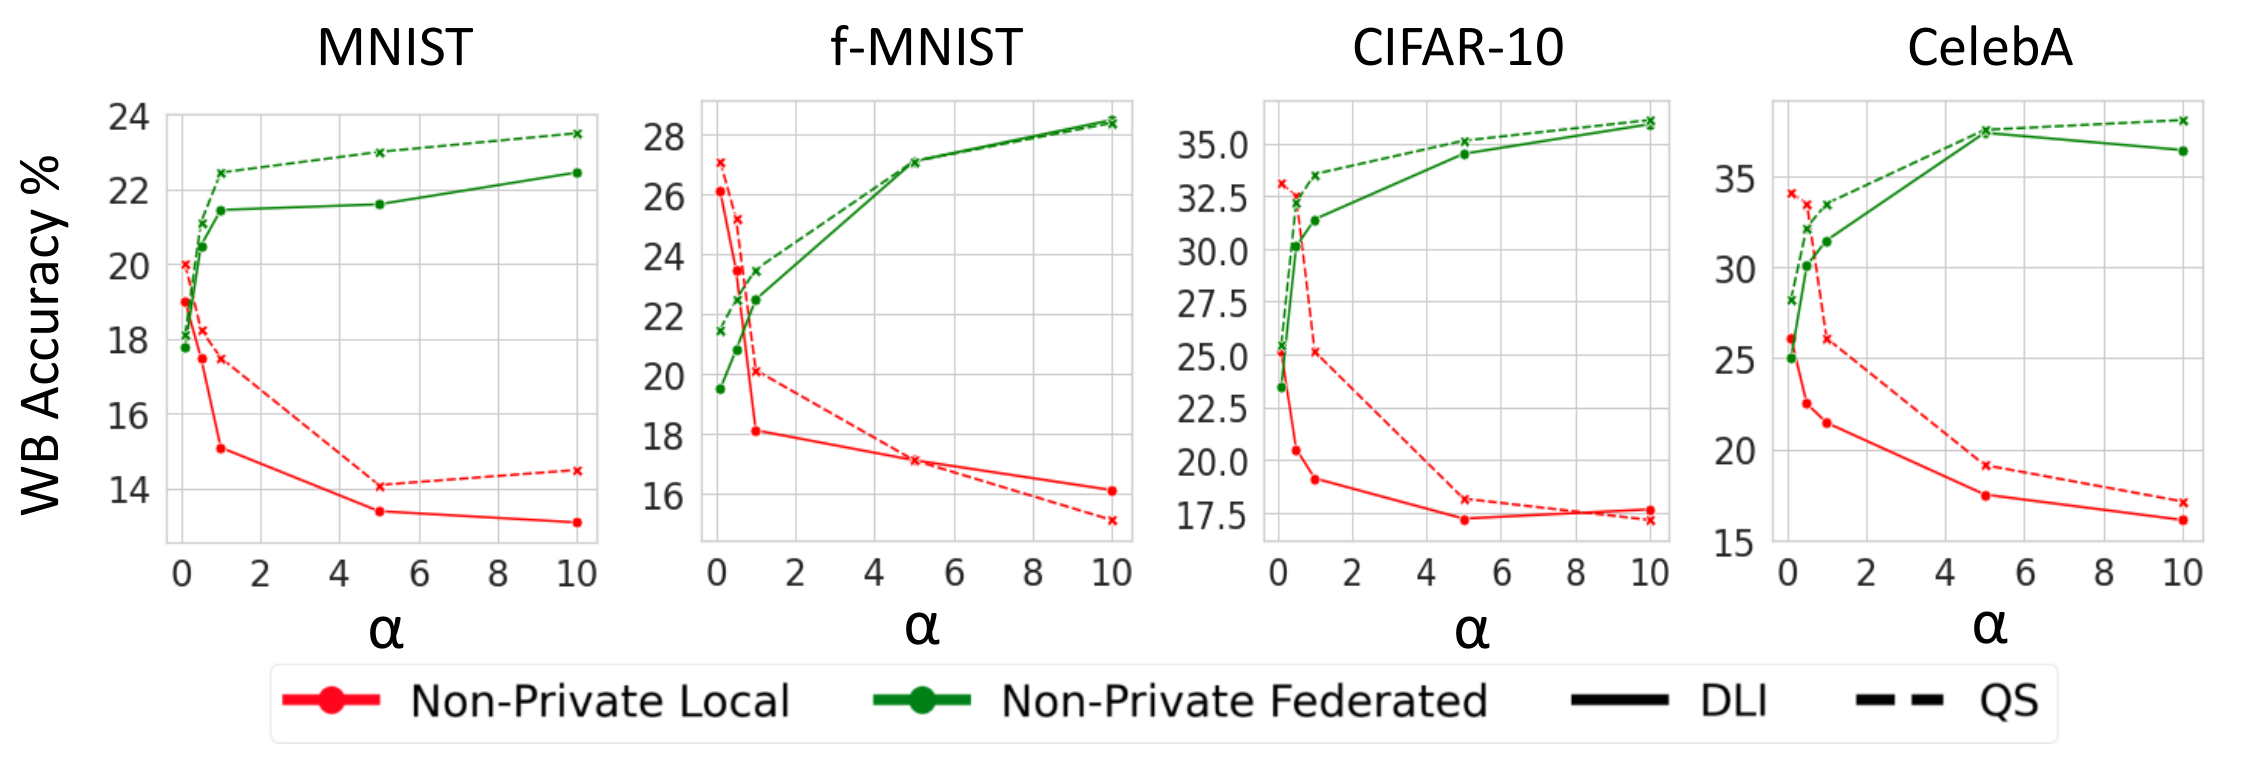
\includegraphics[width=0.8\linewidth]{Plots/nonprivate_vary_alpha_attack.png}
%  \caption{Varying Concentration Parameter for Non-Private Local GANs and Federated GAN: The Figure displays the results of a white-box attack using non-private local GANs and federated GAN with $K=10$ for various concentration parameters.}
%  \label{fig:nonprivate_vary_alpha_attack}
% \end{figure}




% \begin{figure}
%  \centering
%  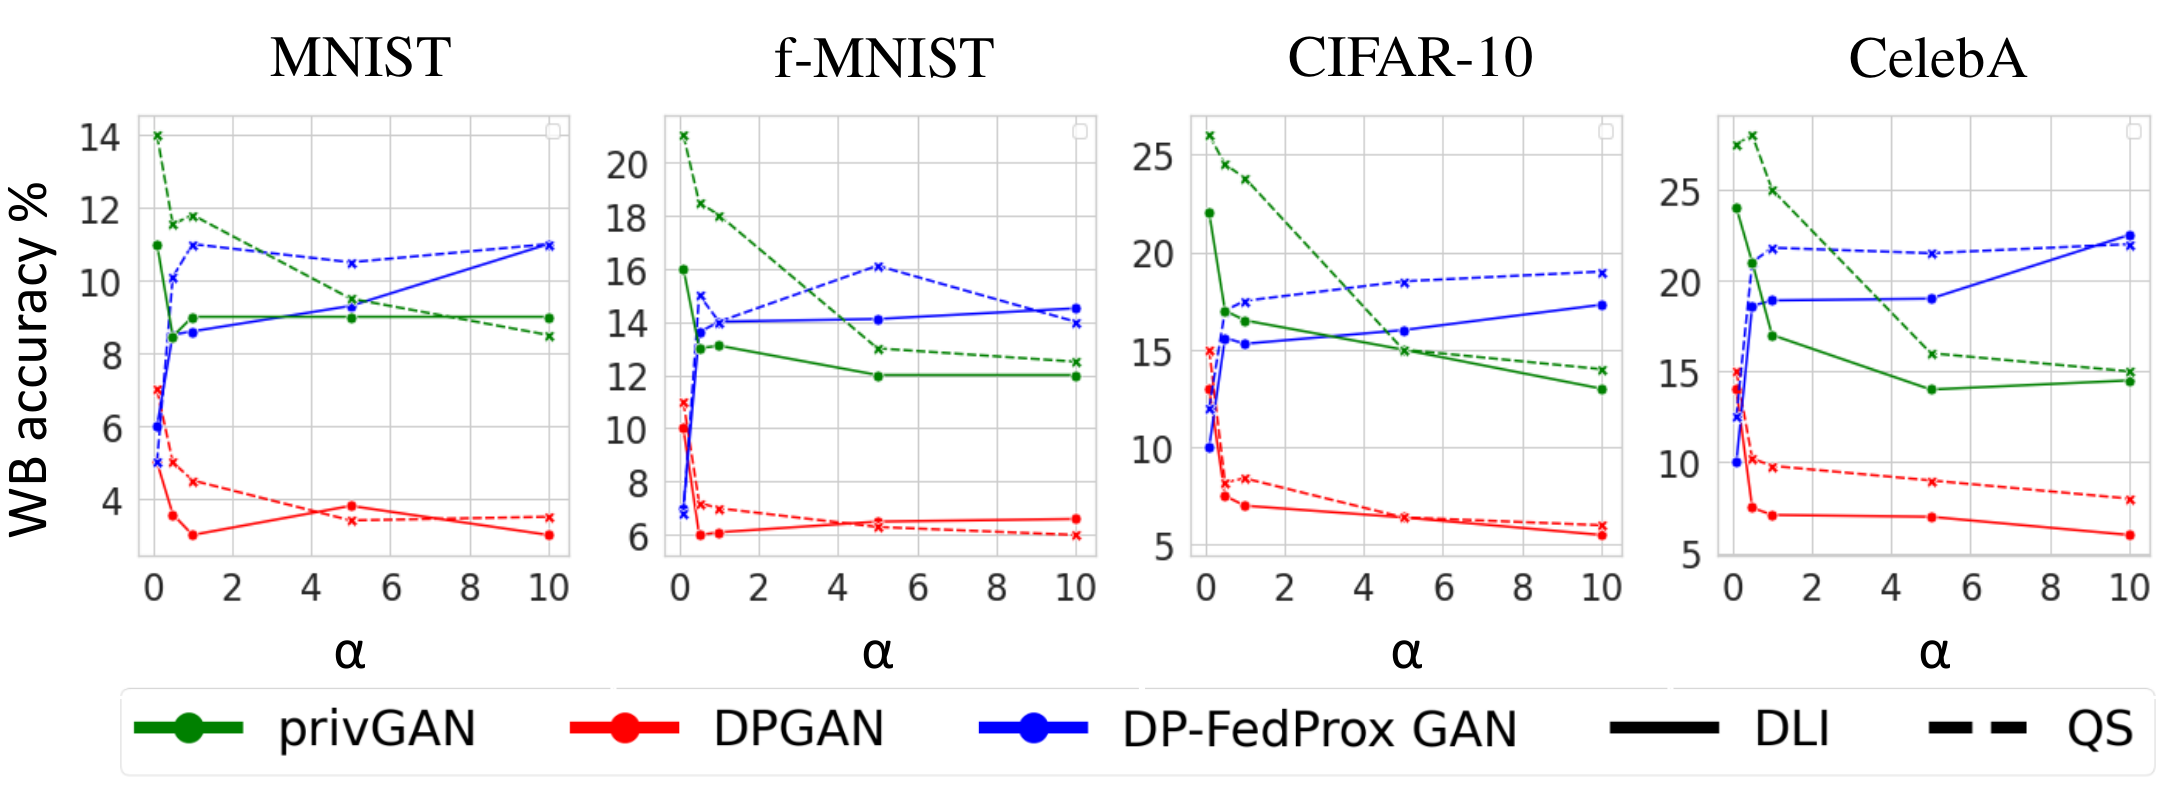
\includegraphics[width=0.8\linewidth]{Plots/vary_alpha_WB.png}
%  \caption{Varying Concentration Parameter: The Figure displays WB Attack at various concentration parameters in privGAN, DPGAN, and DP-FedProx GAN discriminator}
%  \label{fig:vary_alpha_WB}
% \end{figure}








% \begin{figure}
%  \centering
%  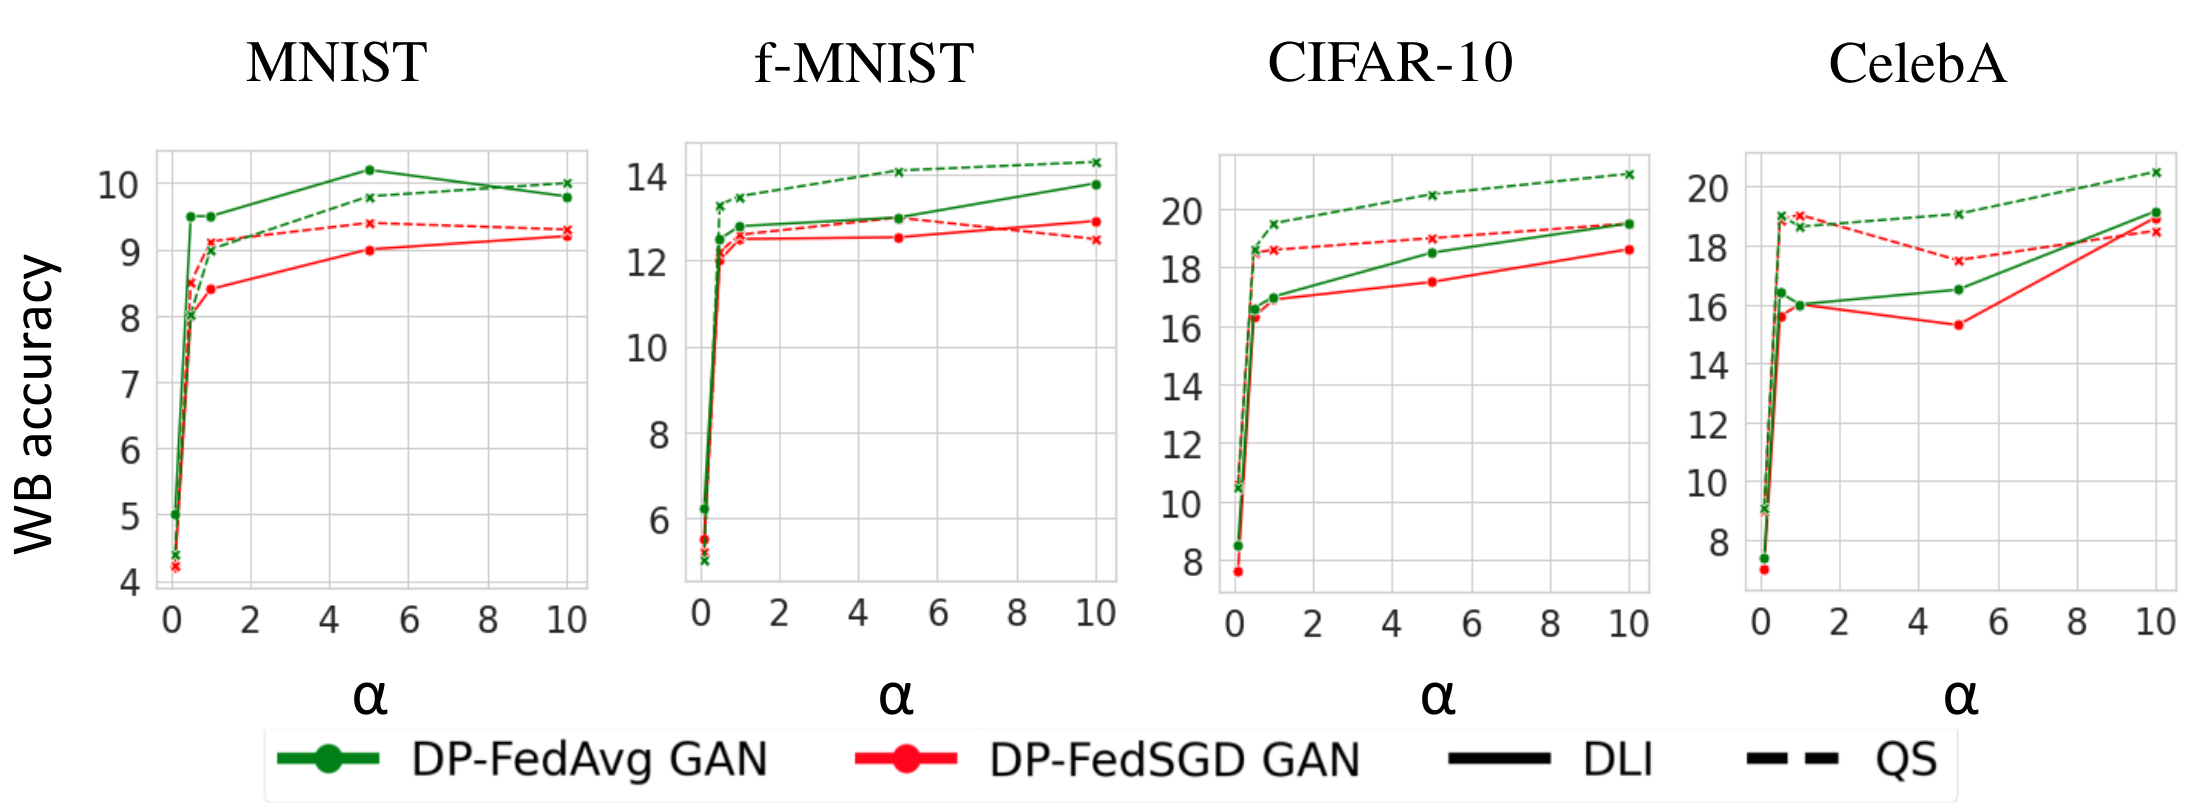
\includegraphics[width=0.8\linewidth]{Plots/vary_alpha_fedsgd_fedavg_WB.png}
%  \caption{Varying Concentration Parameter: The Figure represents WB Attack on discriminator(s) at various concentration parameters in DP-FedAvg GAN and DP-FedSGD GAN. }
%  \label{fig:vary_alpha_fedsgd_fedavg_WB}
% \end{figure}






% \begin{figure}
%  \centering
%  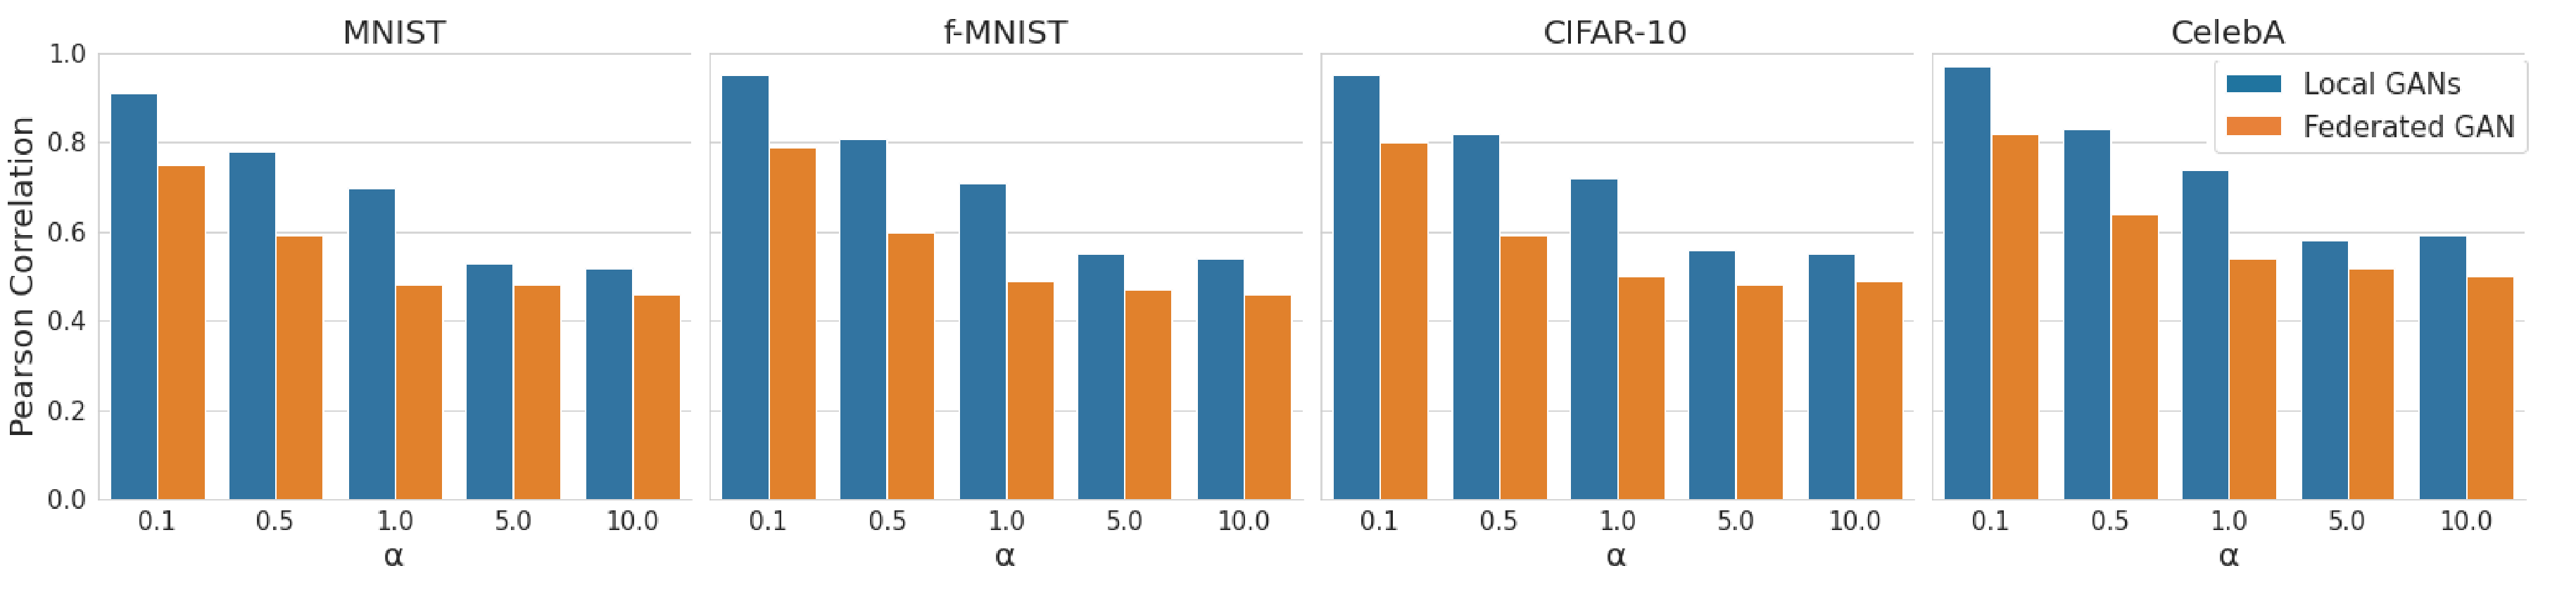
\includegraphics[width=0.8\linewidth]{Plots/WB_alpha_nonprivate.png}
%  \caption{Vary Concentration Parameters in QS distribution: The Figure depicts Pearson correlation $r$ between local data size and local WB accuracy at various concentration parameters $\alpha$ in Local GANs and Federated GAN at $K=10$. }
%  \label{fig:WB_alpha_nonprivate}
% \end{figure}



% \begin{figure}
%  \centering
%  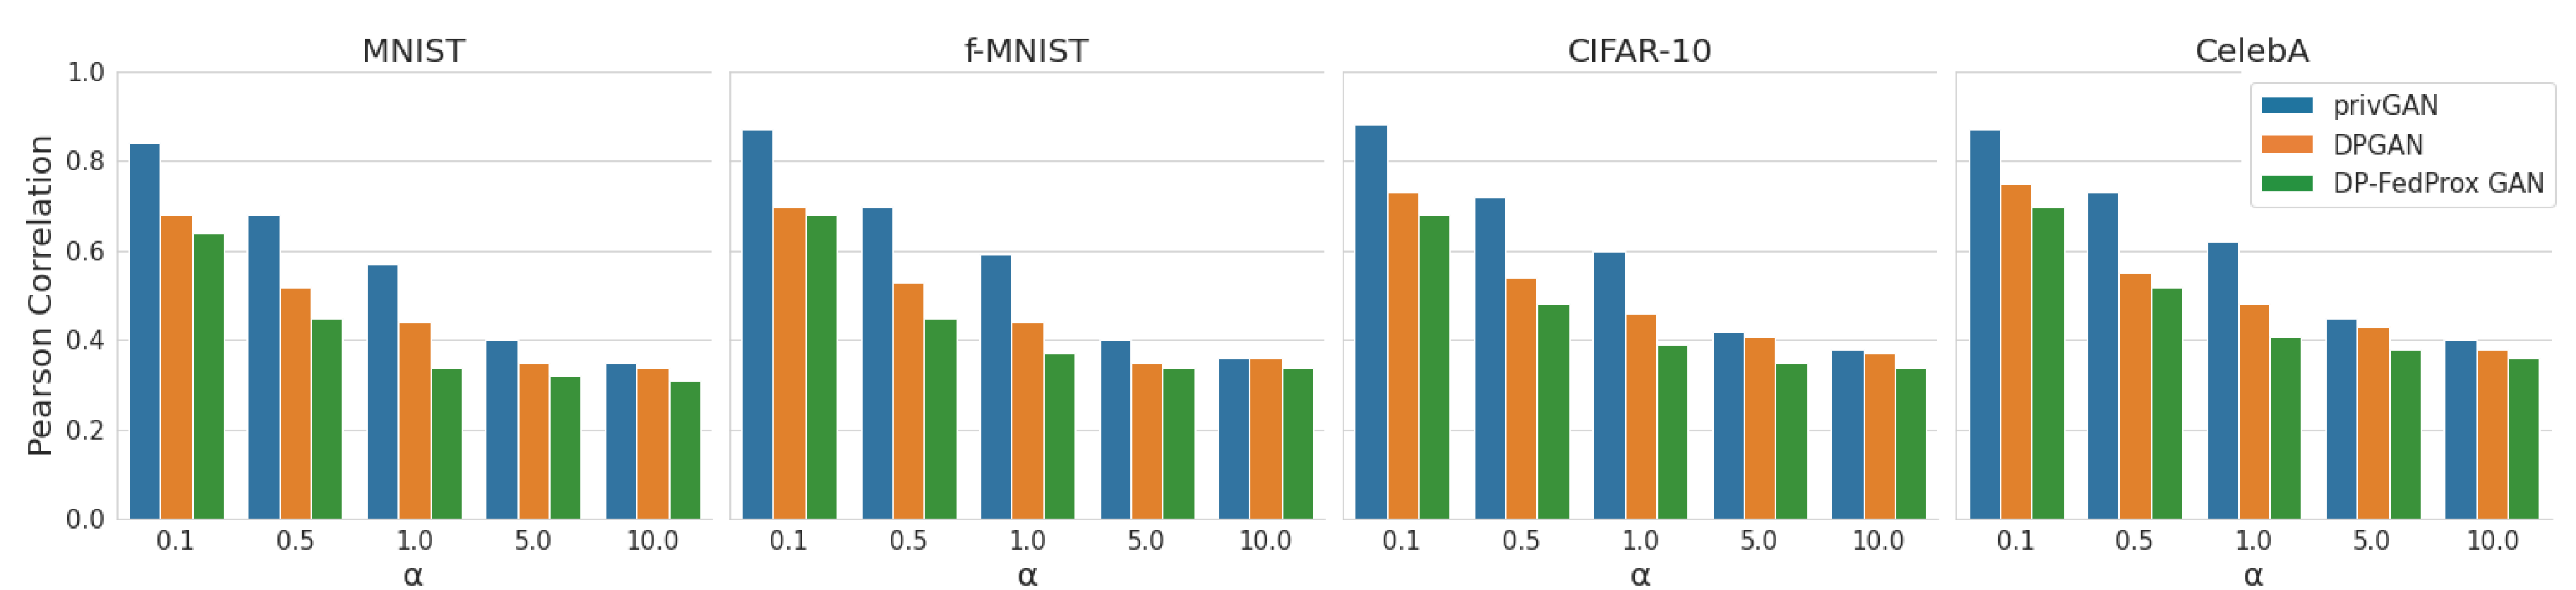
\includegraphics[width=0.8\linewidth]{Plots/Wb_alpha_private.png}
%  \caption{Vary Concentration Parameters in QS distribution: The Figure depicts Pearson correlation $r$ between local data size and local WB accuracy at various concentration parameters $\alpha$ in privGAN, DPGAN, and DP-FedProx GAN.  }
%  \label{fig:Wb_alpha_private}
% \end{figure}


% \begin{figure}
%  \centering
%  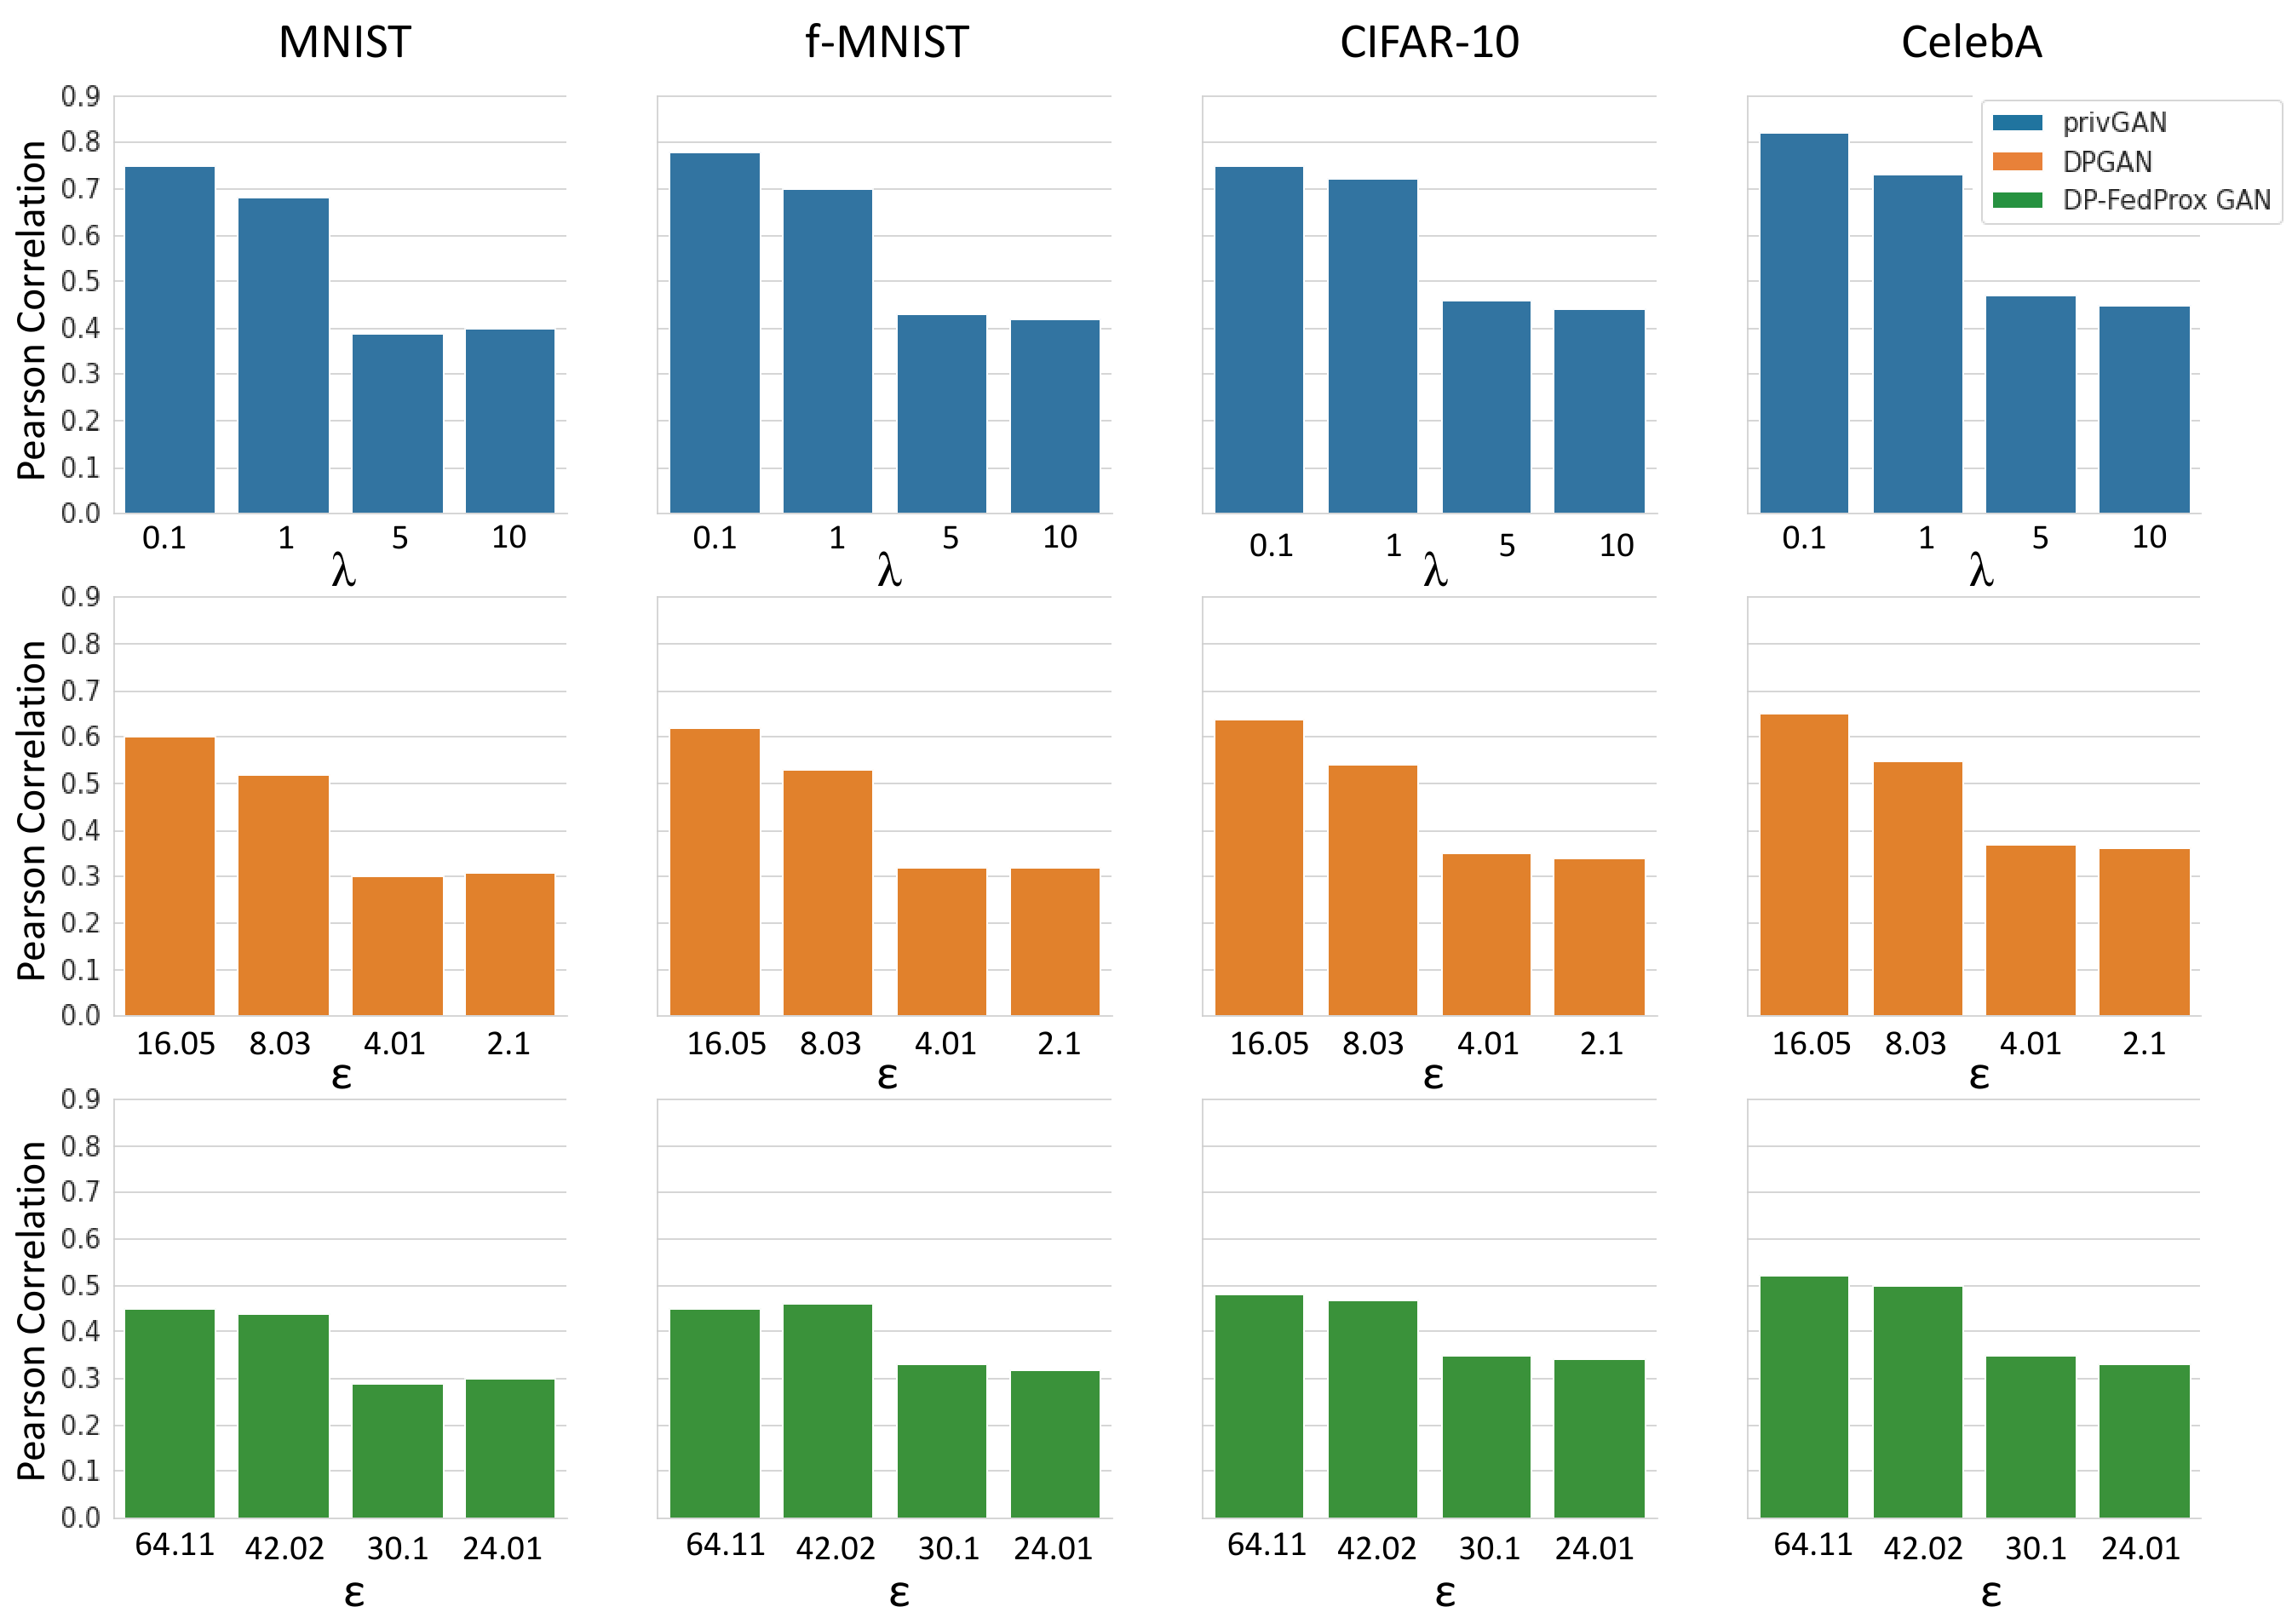
\includegraphics[width=0.8\linewidth]{Plots/Wb_noise_private.png}
%  \caption{Vary Privacy Parameters in QS distribution: The Figure depicts Pearson correlation $r$ between local data size and local WB accuracy at various privacy parameters in privGAN, DPGAN, and DP-FedProx GAN.    }
%  \label{fig:Wb_noise_private}
% \end{figure}












\end{document}
